\chapter{Estado de Arte}
\label{sec:estado-arte}

Neste capítulo será feita uma análise de algumas plataformas existentes para recolha de dados em estratégias de inbound marketing. A recolha de informação nos dias de hoje tem um grande impacto na forma como os negócios são feitos, principalmente na internet. Neste contexto, serão analisadas algumas das soluções que partilham funcionalidades semelhantes com o que vai ser desenvolvido.\\
Como referido no capítulo anterior, o modelo de negócio da plataforma é \gls{b2b} e neste sentido as caracteristicas analisadas serão focadas na segmentação de dados, integração com serviços externos, planos de pagamento e funcionalidades do \textit{back office}.
Seguindo uma das estratégias de inbound marketing, o método de envio de formações e recolha de dados será através da formulários online e por isso mesmo algumas características associadas à experiencia do utilizador, como por exemplo a personalização do formulário, serão também analisadas.


As plataformas a analisar serão: SurveyMonkey\cite{surveymonkey}, Typeform\cite{typeform}, Google Forms\cite{googleform}

Após a apresentação destas ferramentas será feita uma análise das vantagens e desvantagens de cada uma, assim como a comparação de funcionalidades.


\section{SurveyMonkey}
\label{surveyMonkey}

O SurveyMonkey é uma plataforma \acrfull{saas} de criação de formulários online. Permite recolher informações do público alvo através de formulários e personalizados e segmentar e visualizer esta informação.

O SurveyMonkey é uma plataforma que dispões de diversos planos de pagamento, e por isso mesmo, apesar de estar disponível um plano gratuito, tem acesso apenas a algumas das funcionalidades e em cada formulário, no máximo, poderá ter 10 perguntas ou elementos.

É necessário criar conta para aceder às funcionalidades da plataforma, dando a opção de utilizar serviços externos para esse efeito (e. g. Facebook\cite{face}, LinkedIn\cite{linkedin}), como podemos ver na Figura \ref{fig:surveymonkey-singin}.

  

\begin{figure}[ht!]
	\begin{center}
		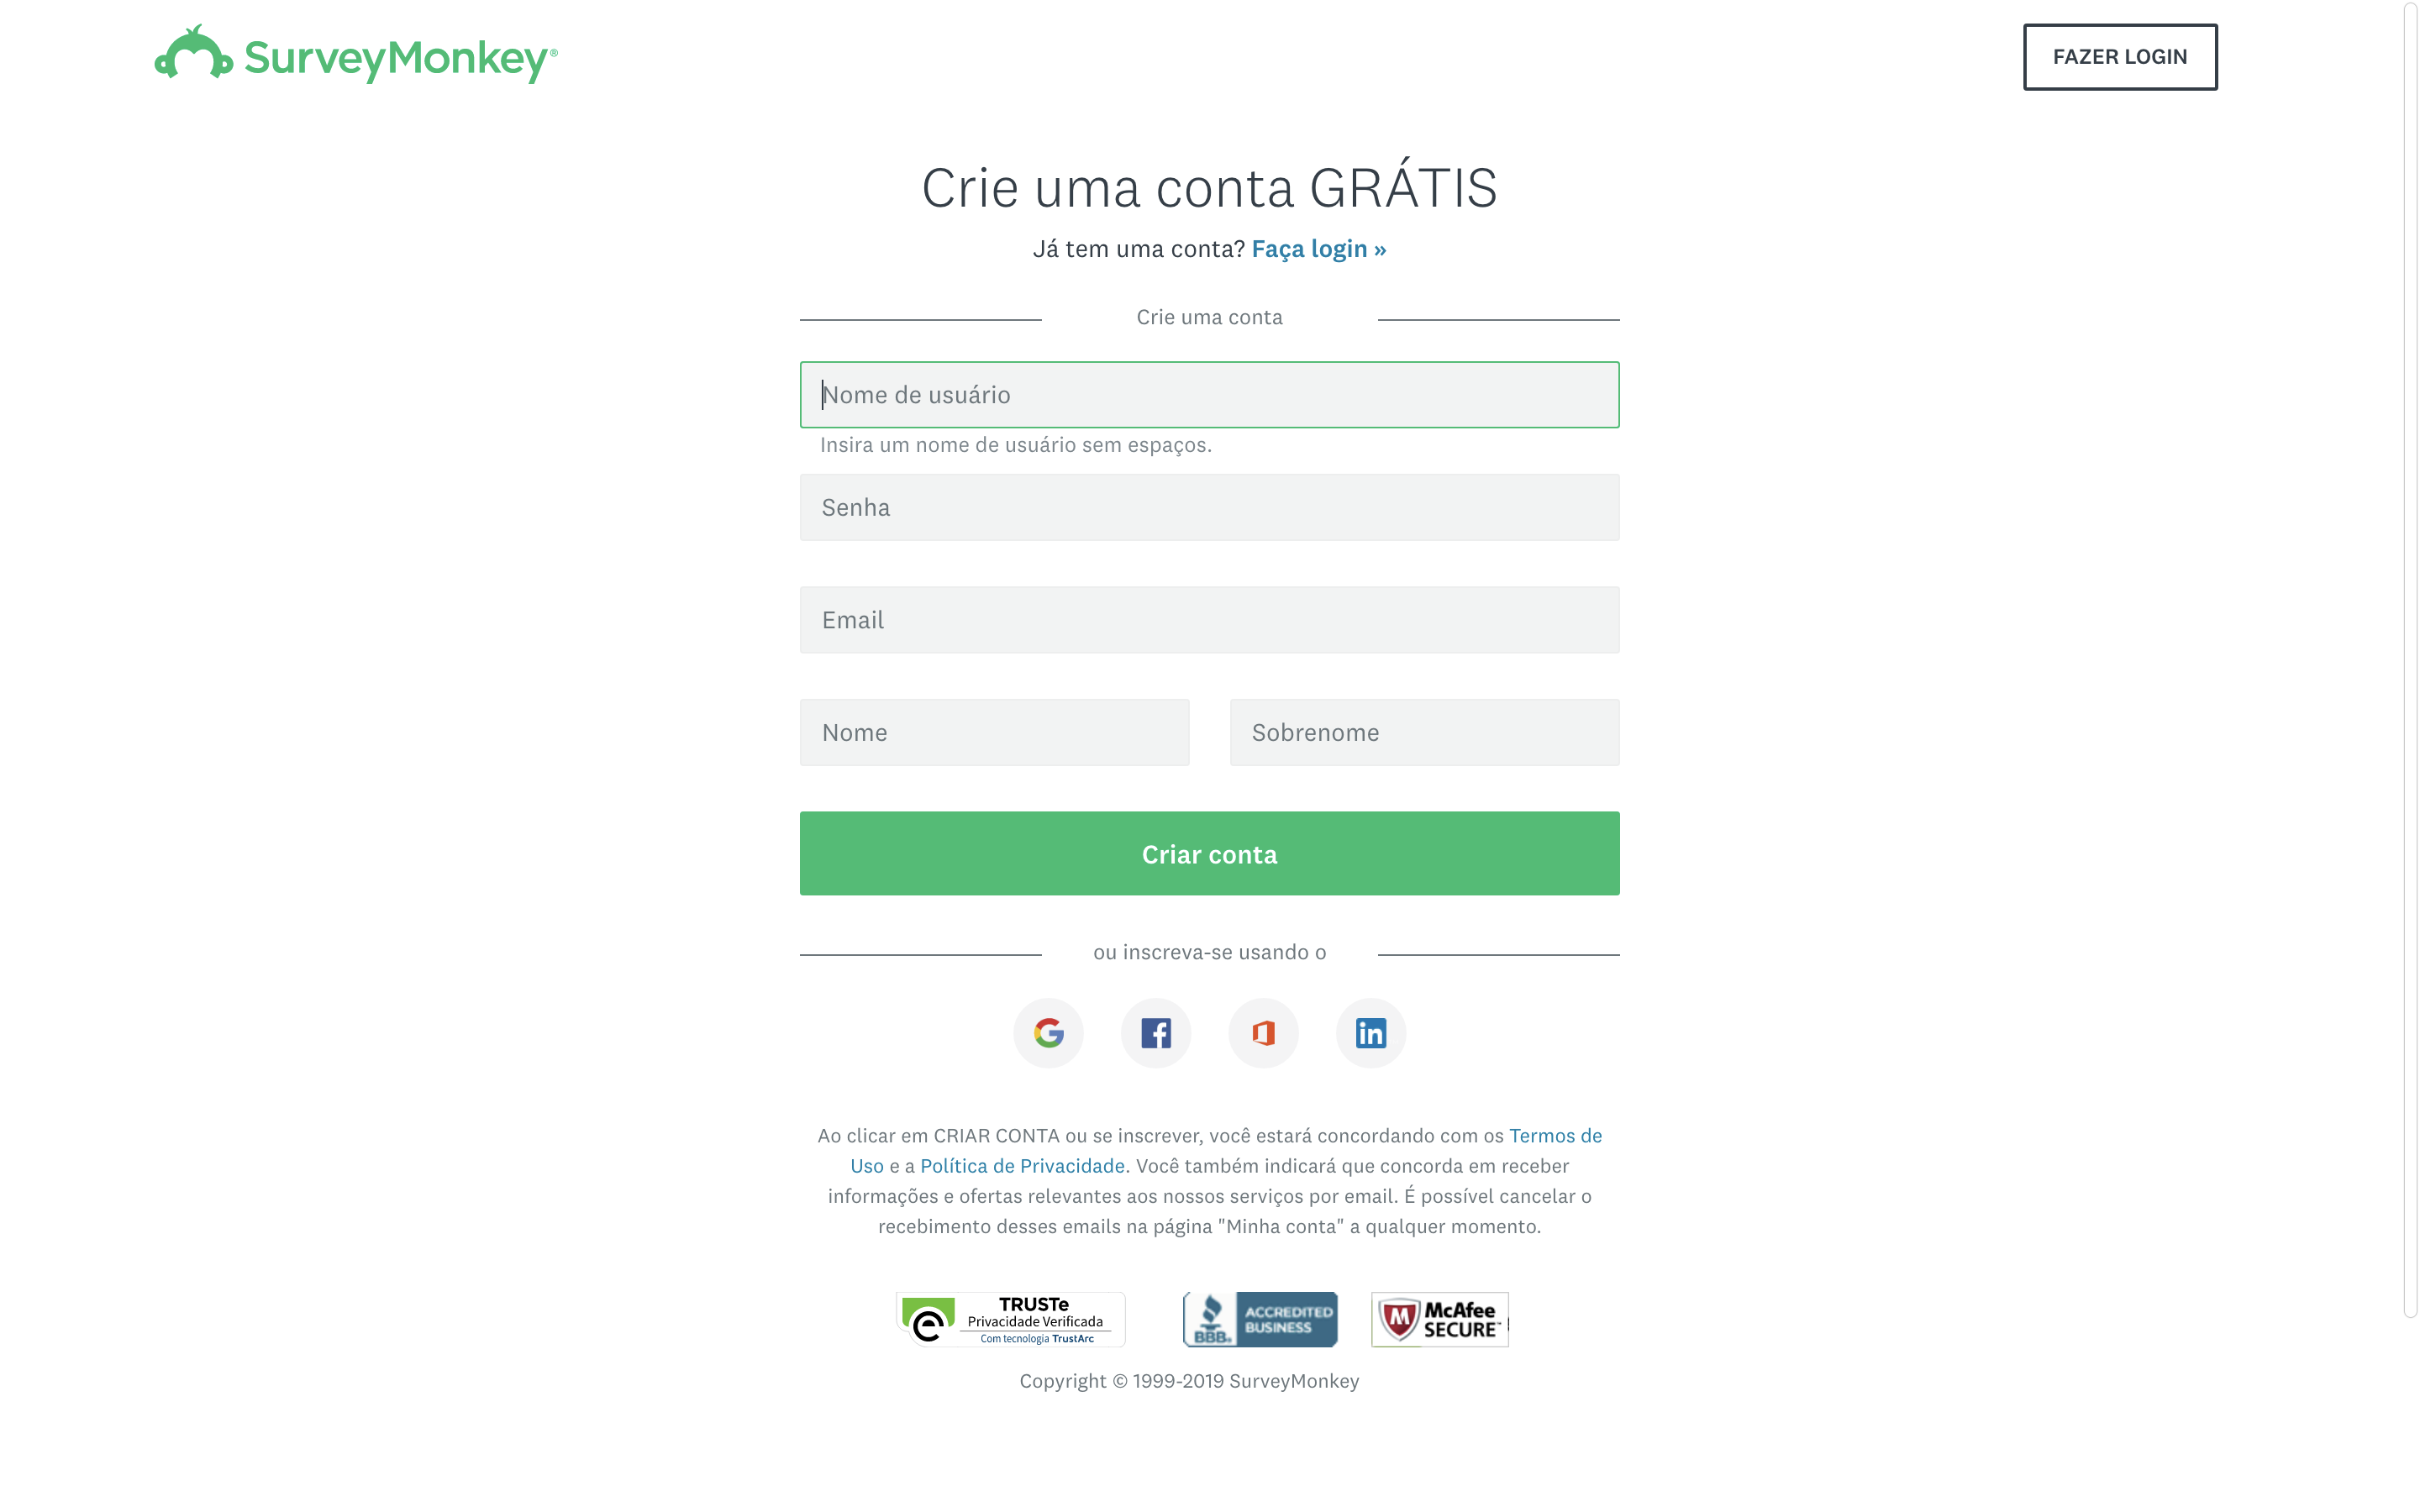
\includegraphics[width=1\textwidth]{img/sm/surveymonkey-singin}
		\caption{SurveyMonkey - Registro }
		\label{fig:surveymonkey-singin}
	\end{center}
\end{figure}

\newpage

No painel principal, como podemos ver na Figura \ref{fig:survey-dashboard} temos acesso rápido aos formulários recentes e a algumas métricas sobre os mesmos. Outra forma será aceder aos formulários do utilizador através da barra de navegação. 


\begin{figure}[ht!]
	\begin{center}
		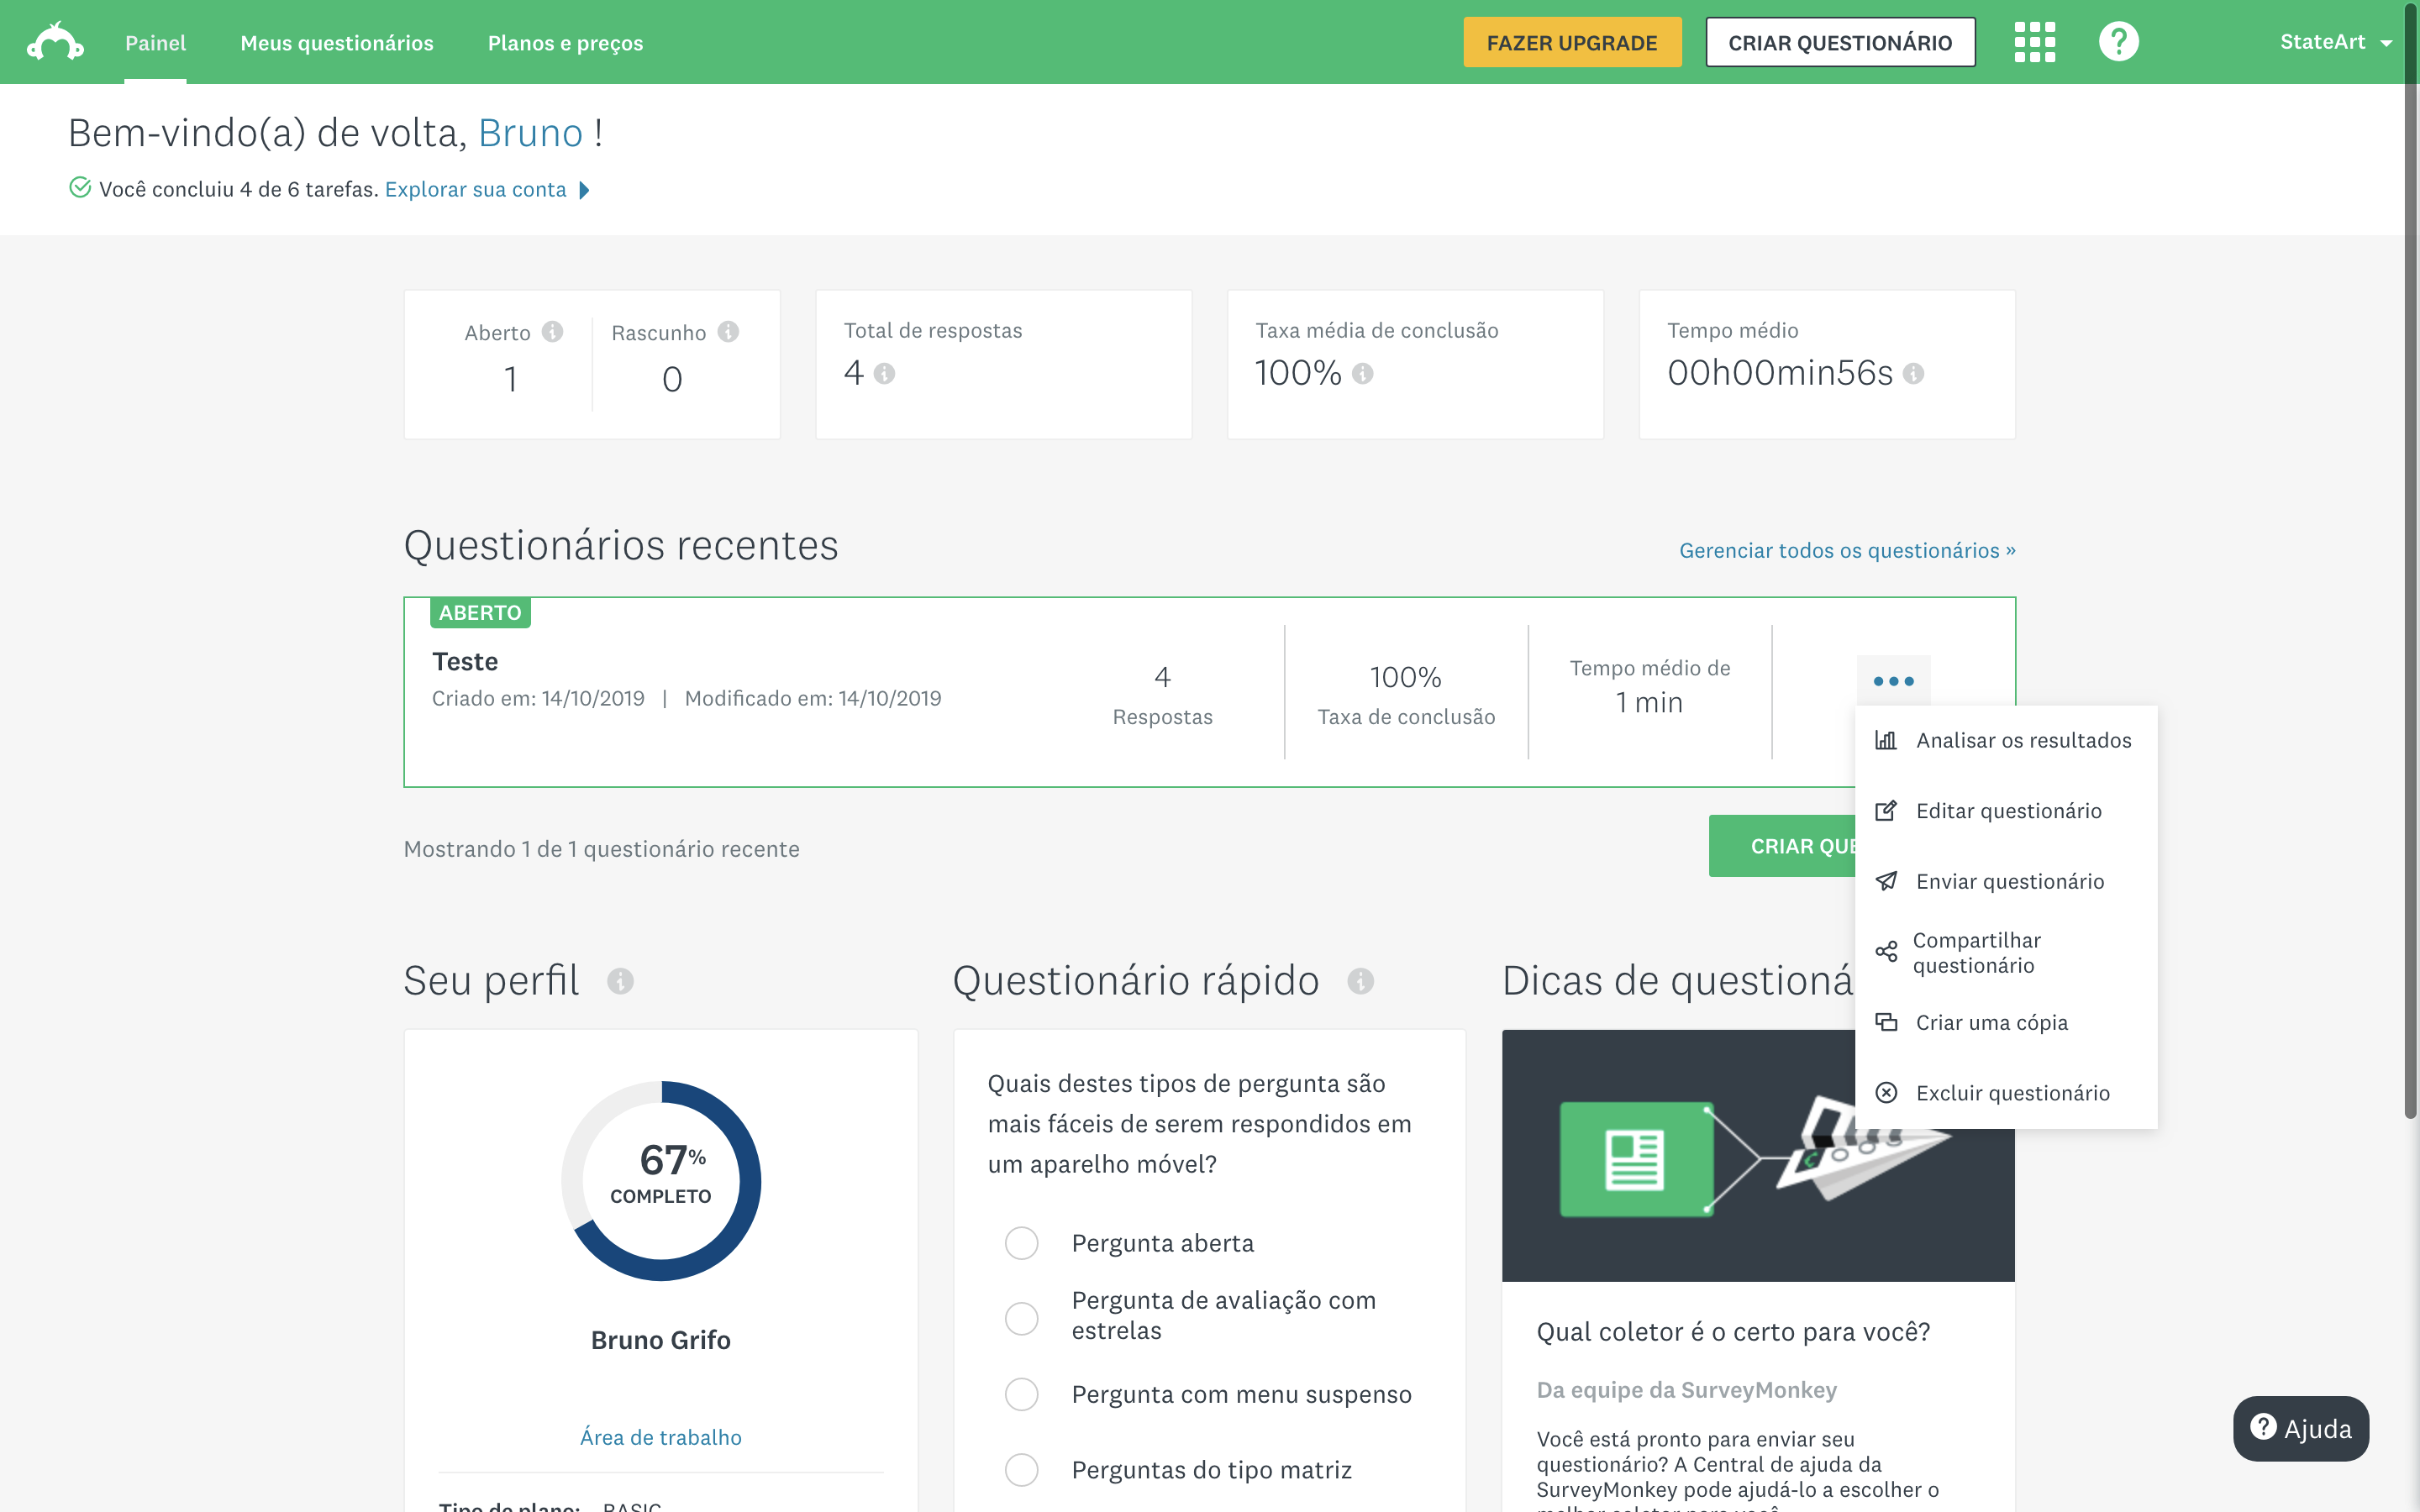
\includegraphics[width=1\textwidth]{img/sm/survey-dashboard}
		\caption{SurveyMonkey - Painel de Controle }
		\label{fig:survey-dashboard}
	\end{center}
\end{figure}

\newpage

\begin{figure}[ht!]
	\begin{center}
		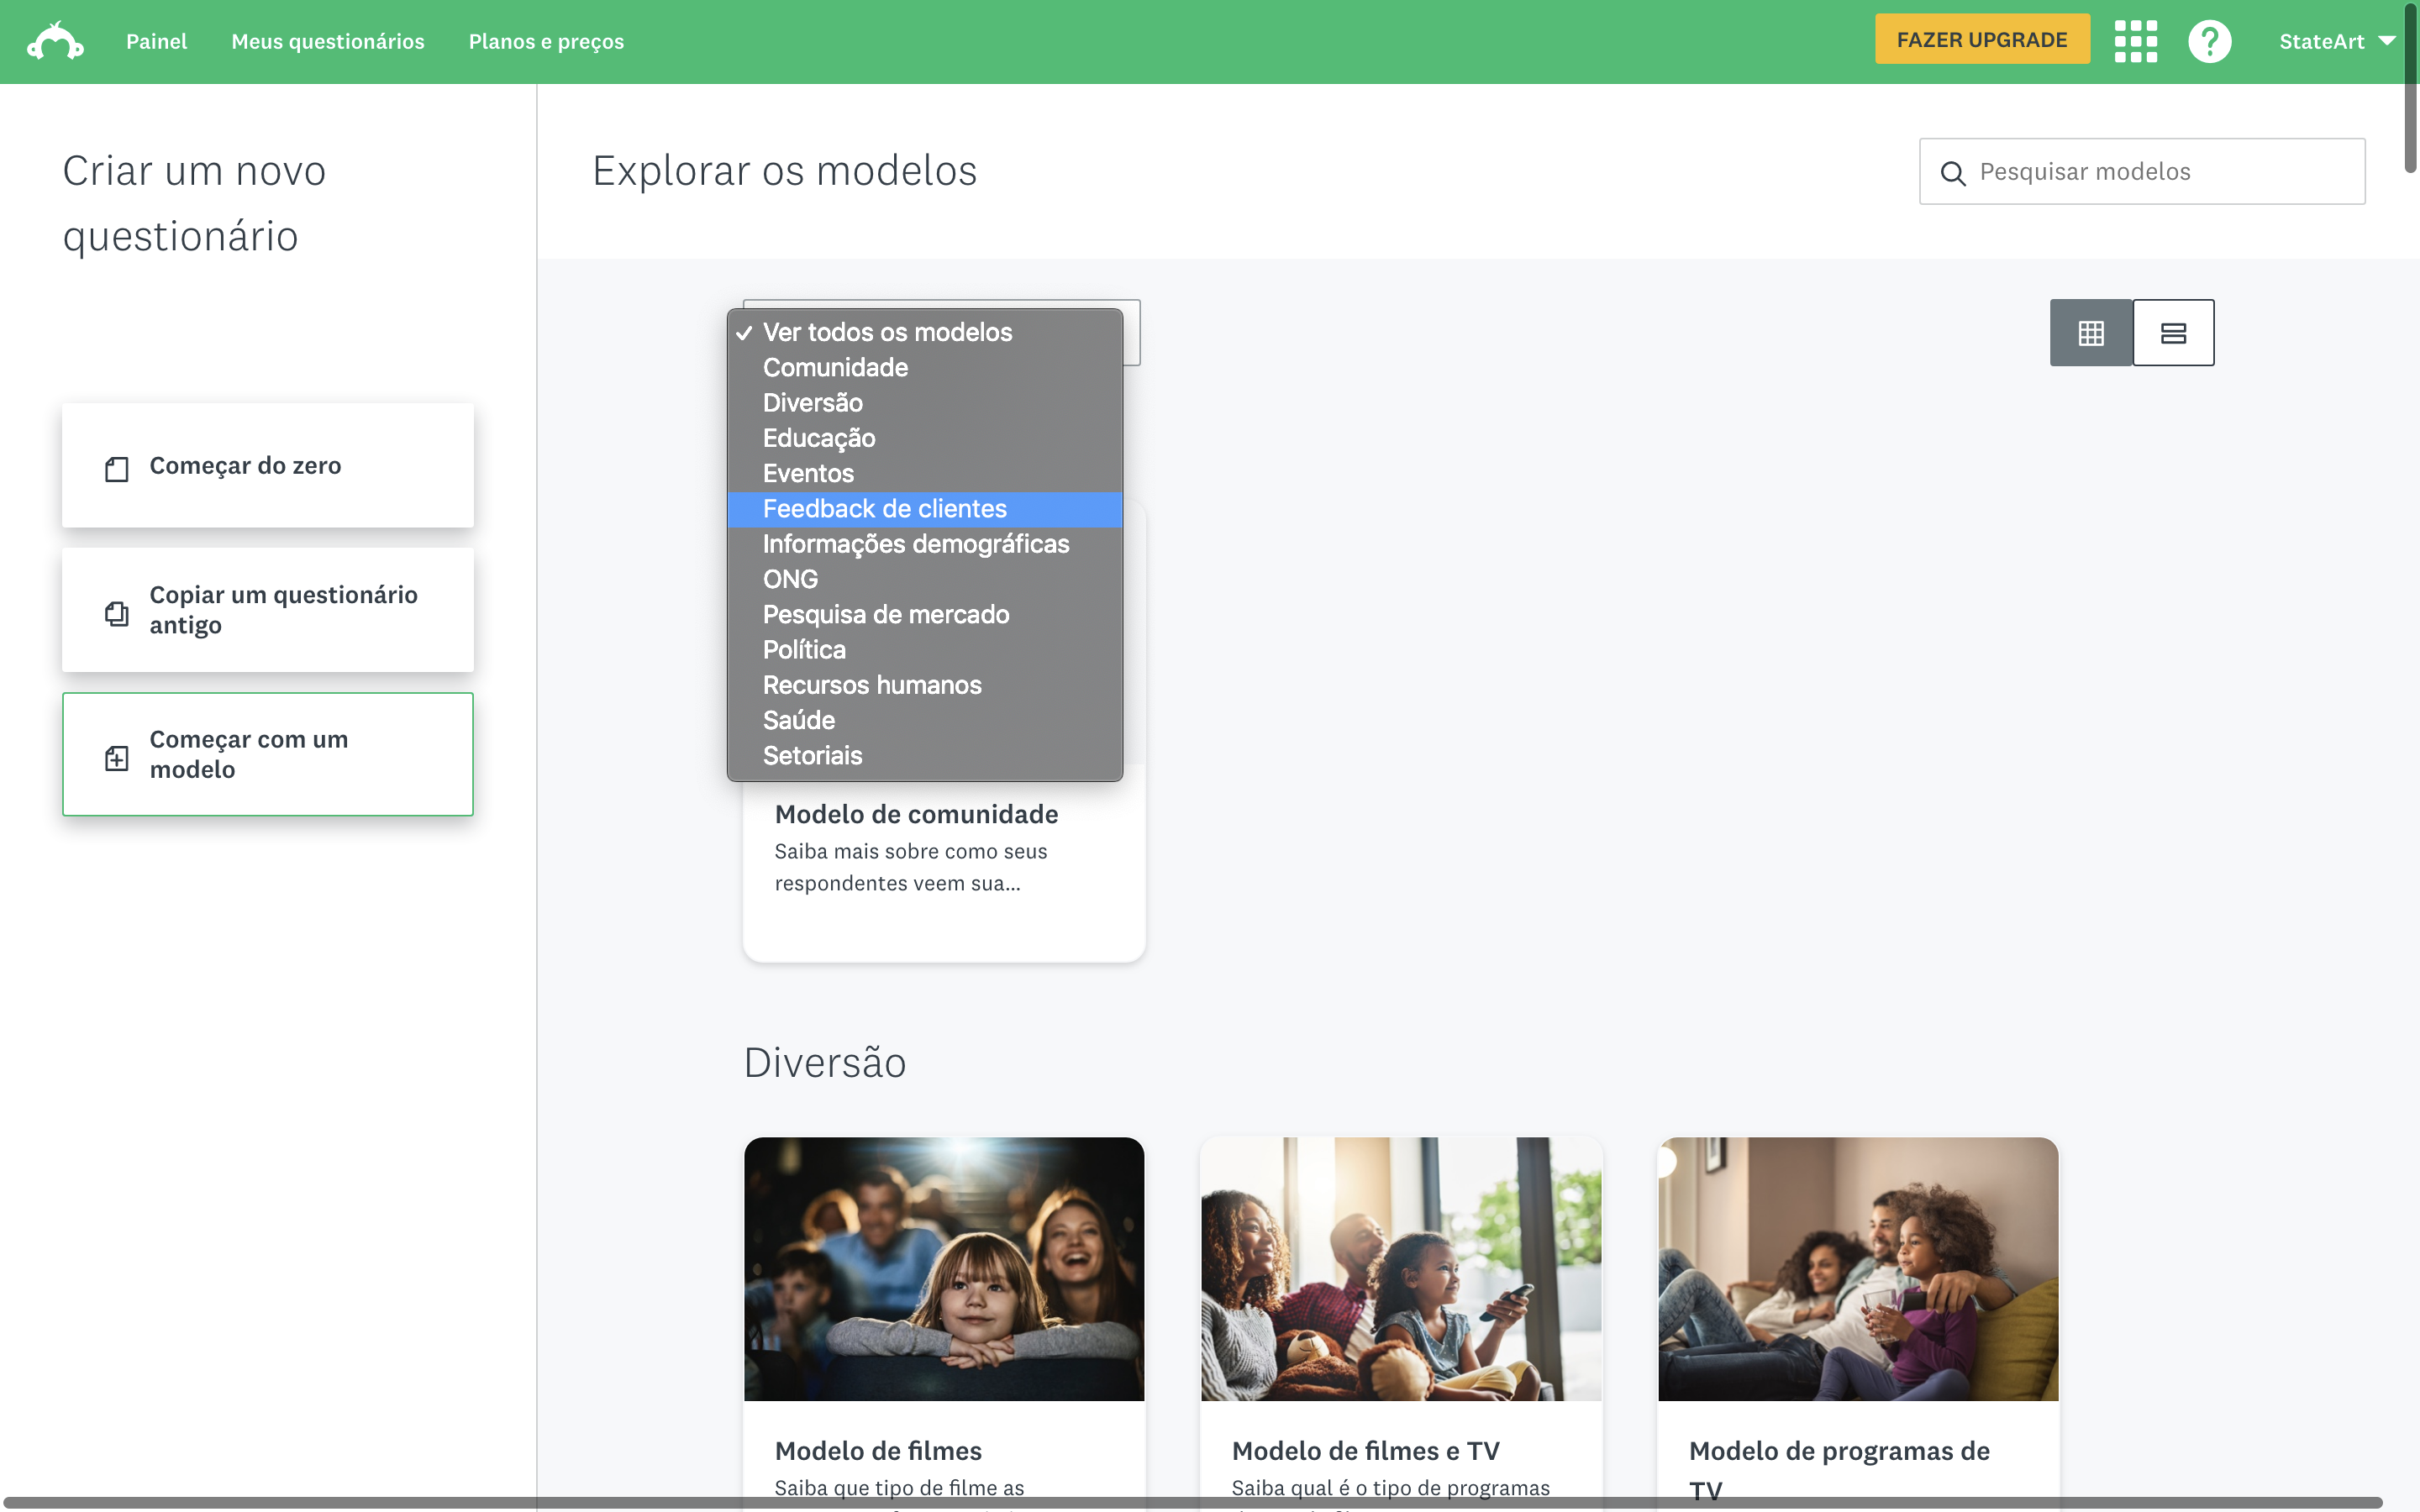
\includegraphics[width=1\textwidth]{img/sm/survey-form-create}
		\caption{SurveyMonkey - Formulários modelo }
		\label{fig:survey-form-create}
	\end{center}
\end{figure}

Quando se inicializa a criação de um novo formulário, a plataforma dá opção de começar do zero ou de utilizar um formulário modelo como podemos ver na Figura \ref{fig:survey-form-create}. Começando um formulário do zero como podemos ver na Figura \ref{fig:survey-form-banck2}, temos acesso a uma série de funcionalidades que vamos explorar e analisar em seguida.

\begin{figure}[ht!]
	\begin{center}
		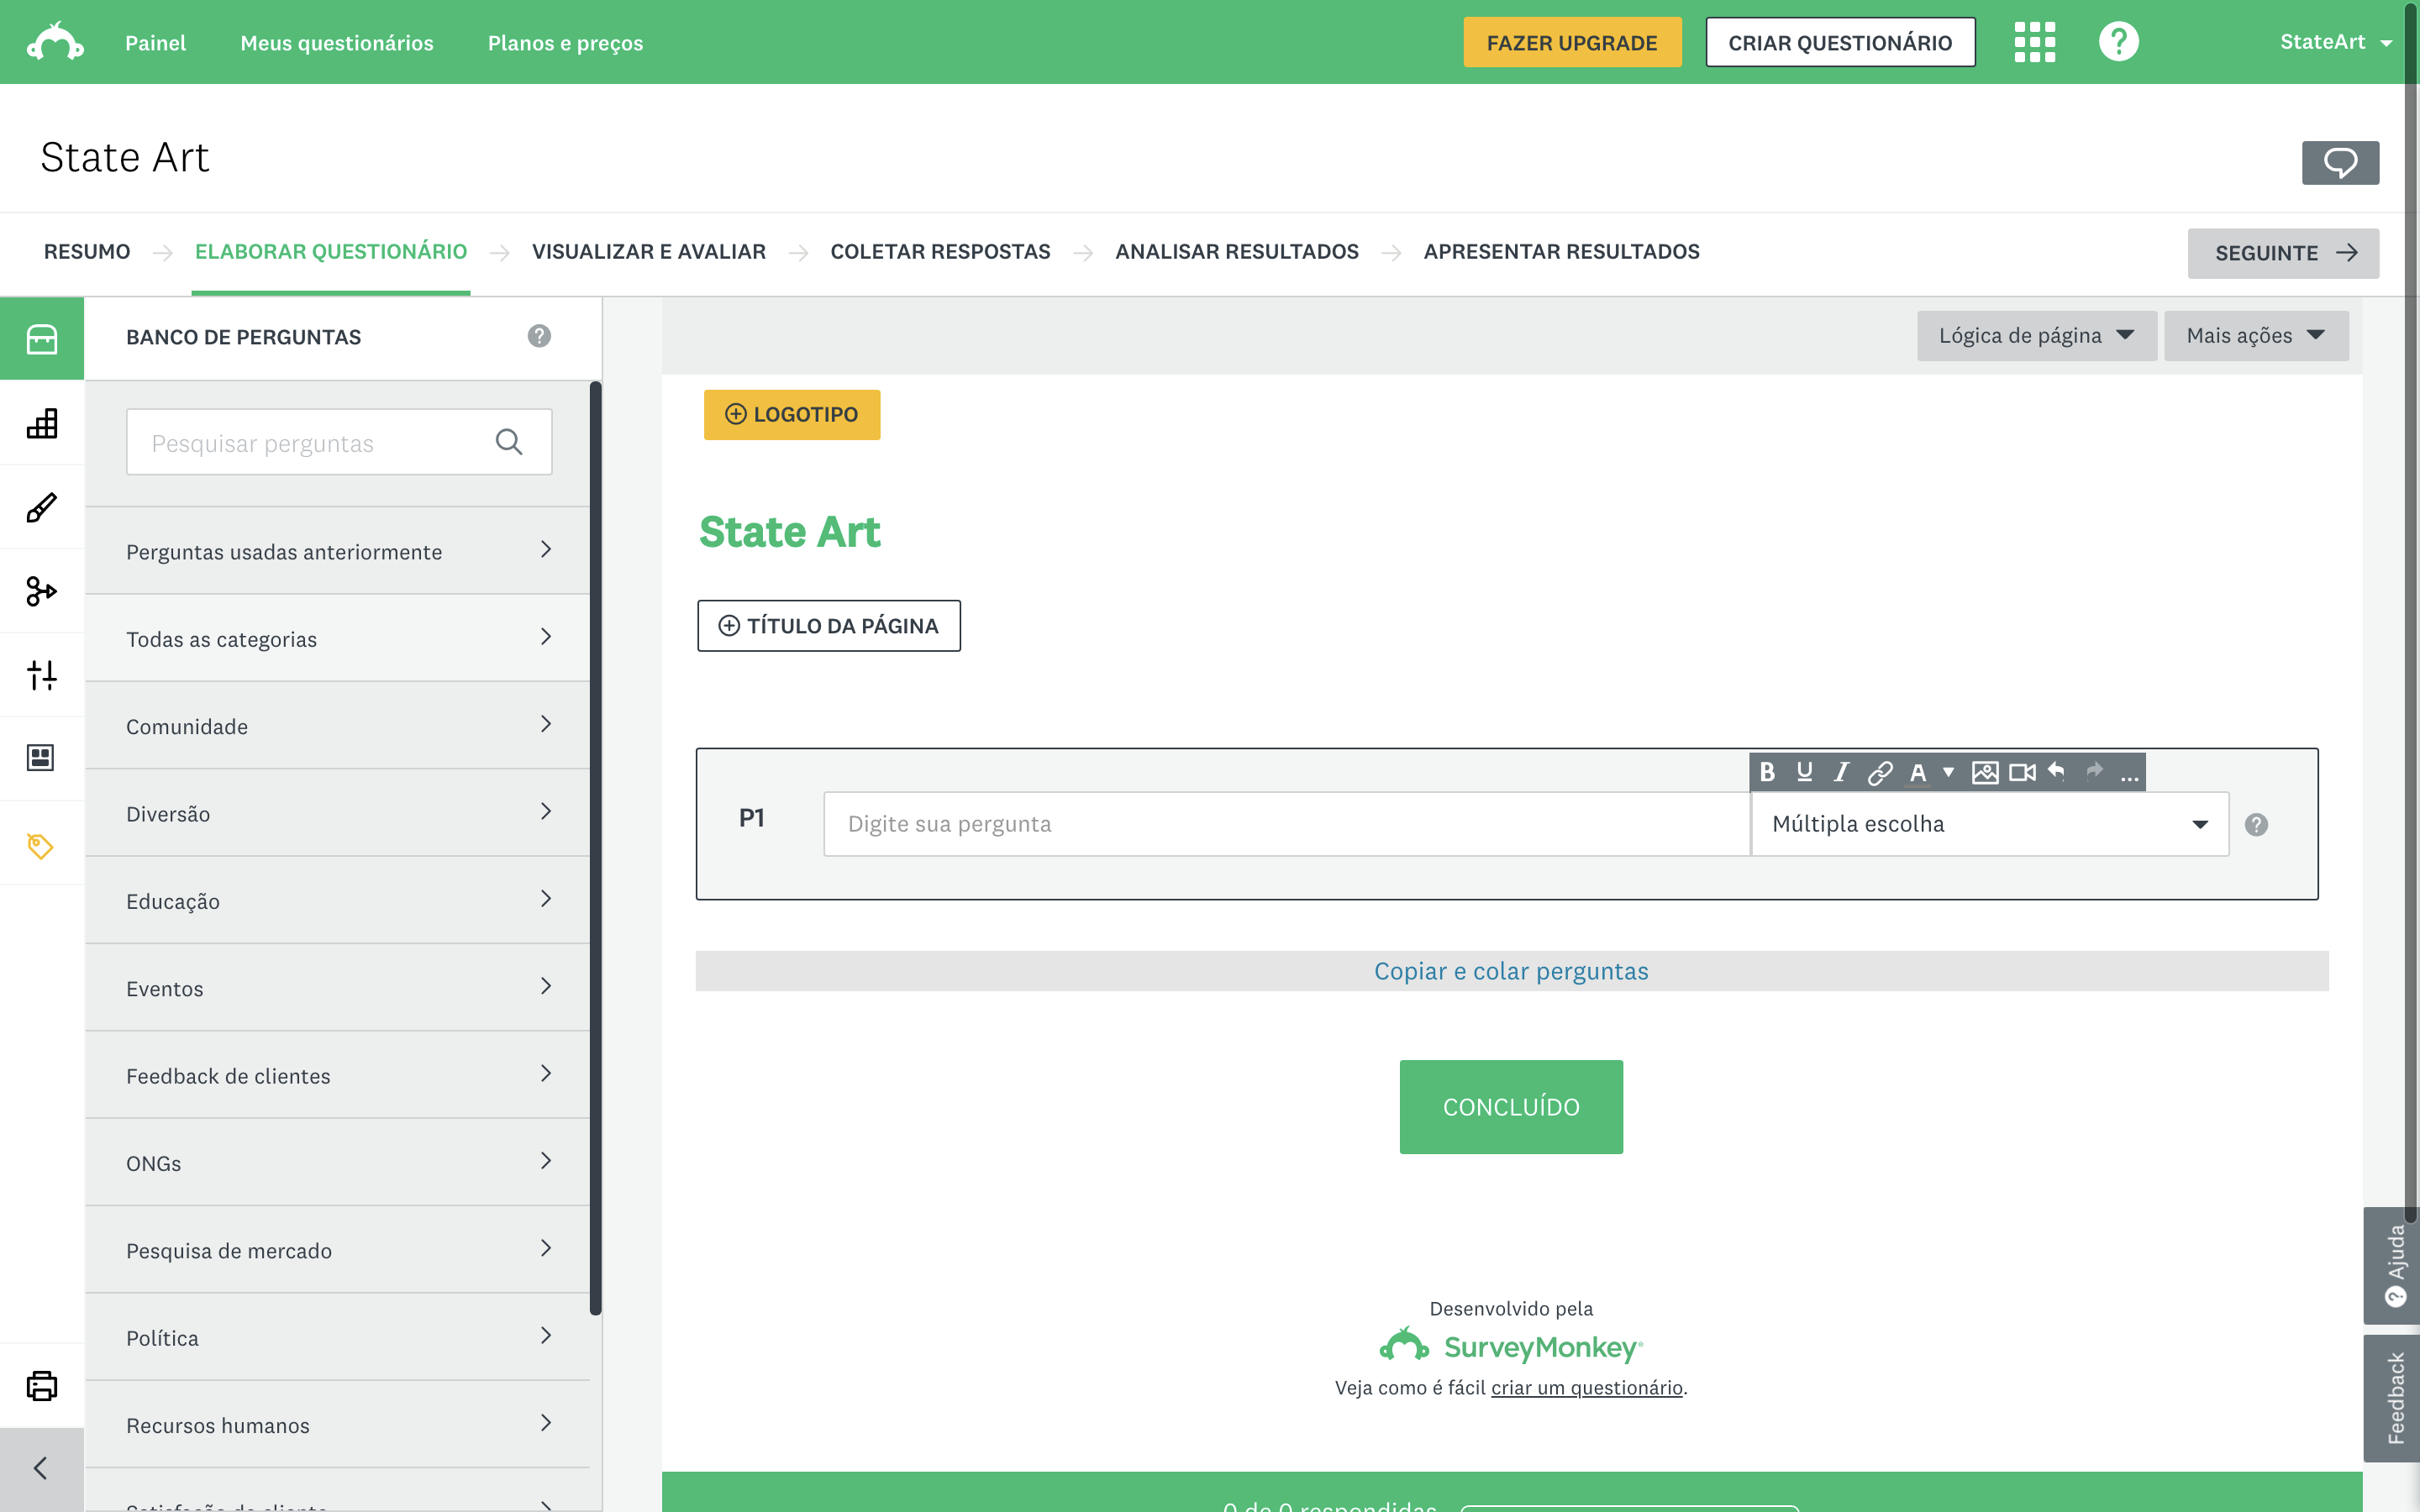
\includegraphics[width=1\textwidth]{img/sm/survey-form-bank2}
		\caption{SurveyMonkey -  Perguntas Modelo}
		\label{fig:survey-form-banck2}
	\end{center}
\end{figure}


\begin{figure}[ht!]
	\begin{center}
		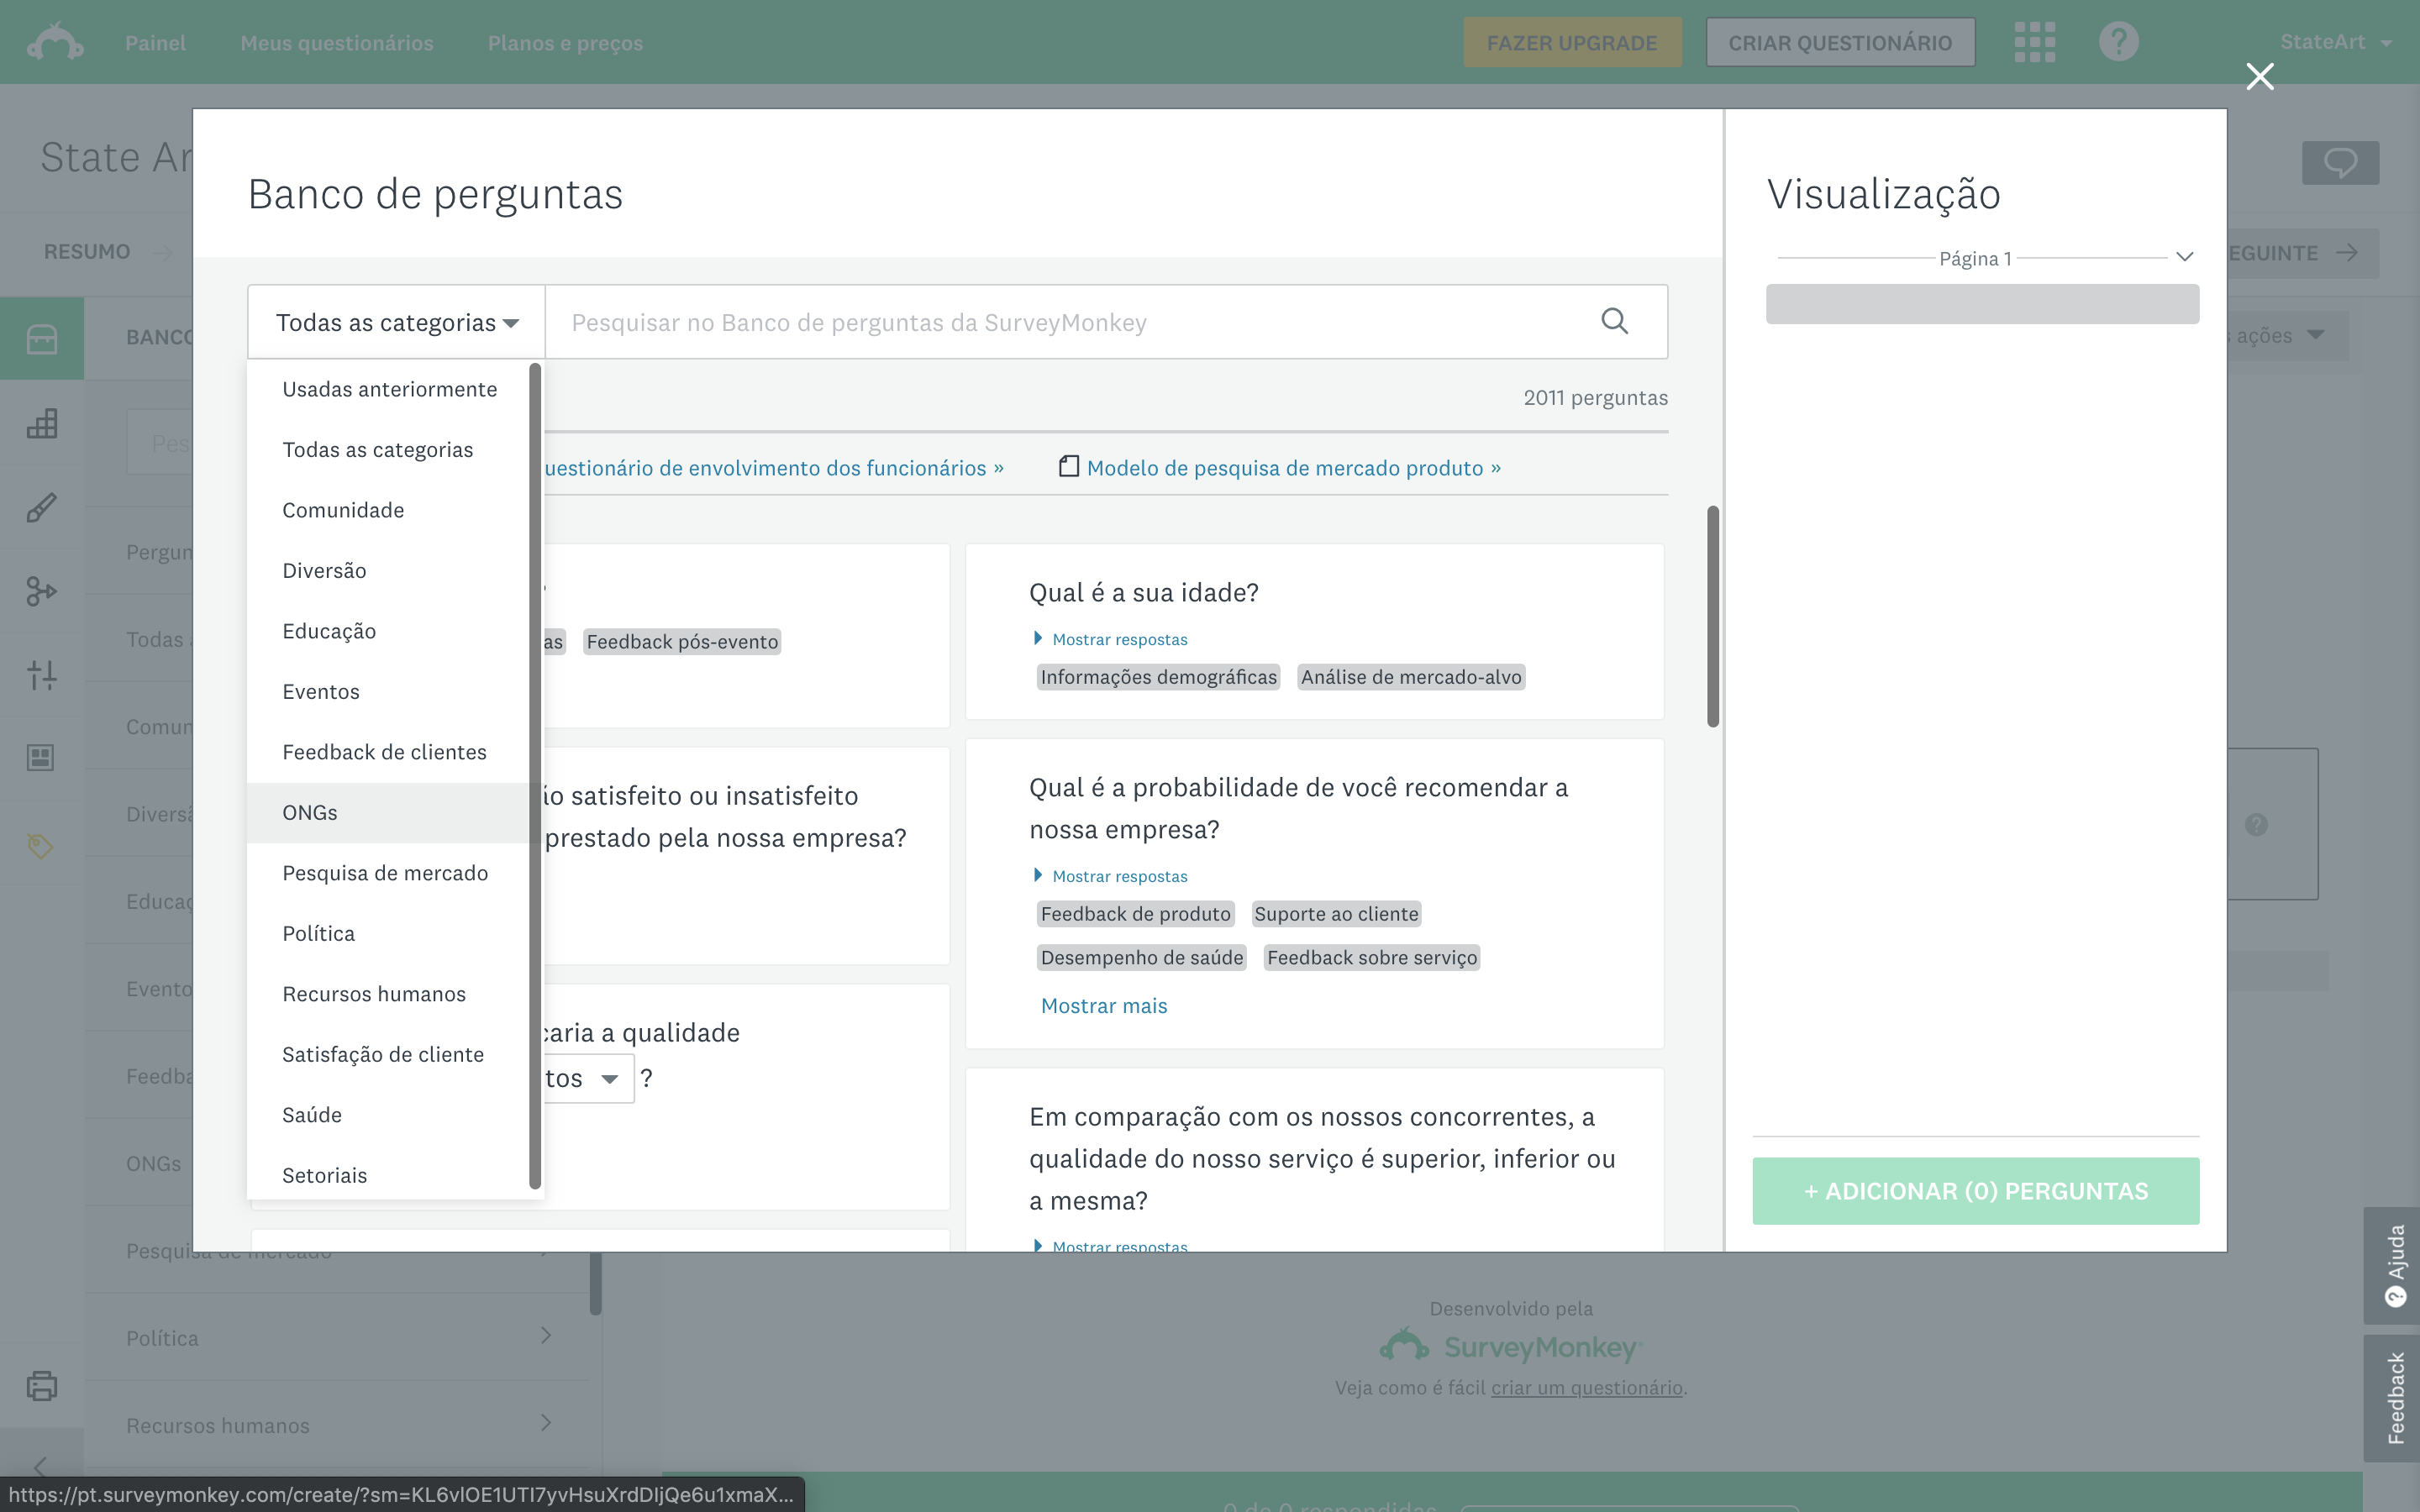
\includegraphics[width=1\textwidth]{img/sm/survey-form-bank1}
		\caption{SurveyMonkey - Perguntas Modelo }
		\label{fig:survey-form-banck1}
	\end{center}
\end{figure}

\newpage

São diversos os elementos que se podem adicionar ou arrastar para o formulário (i. e. perguntas, escolha multipla, imagens...) como representado na Figura \ref{fig:surveymonkey-form-element} e há também um banco de perguntas modelo/recomendações já construídas, organizadas por categorias como podemos ver na Figura \ref{fig:survey-form-banck2} e \ref{fig:survey-form-banck1}.


\begin{figure}[ht!]
	\begin{center}
		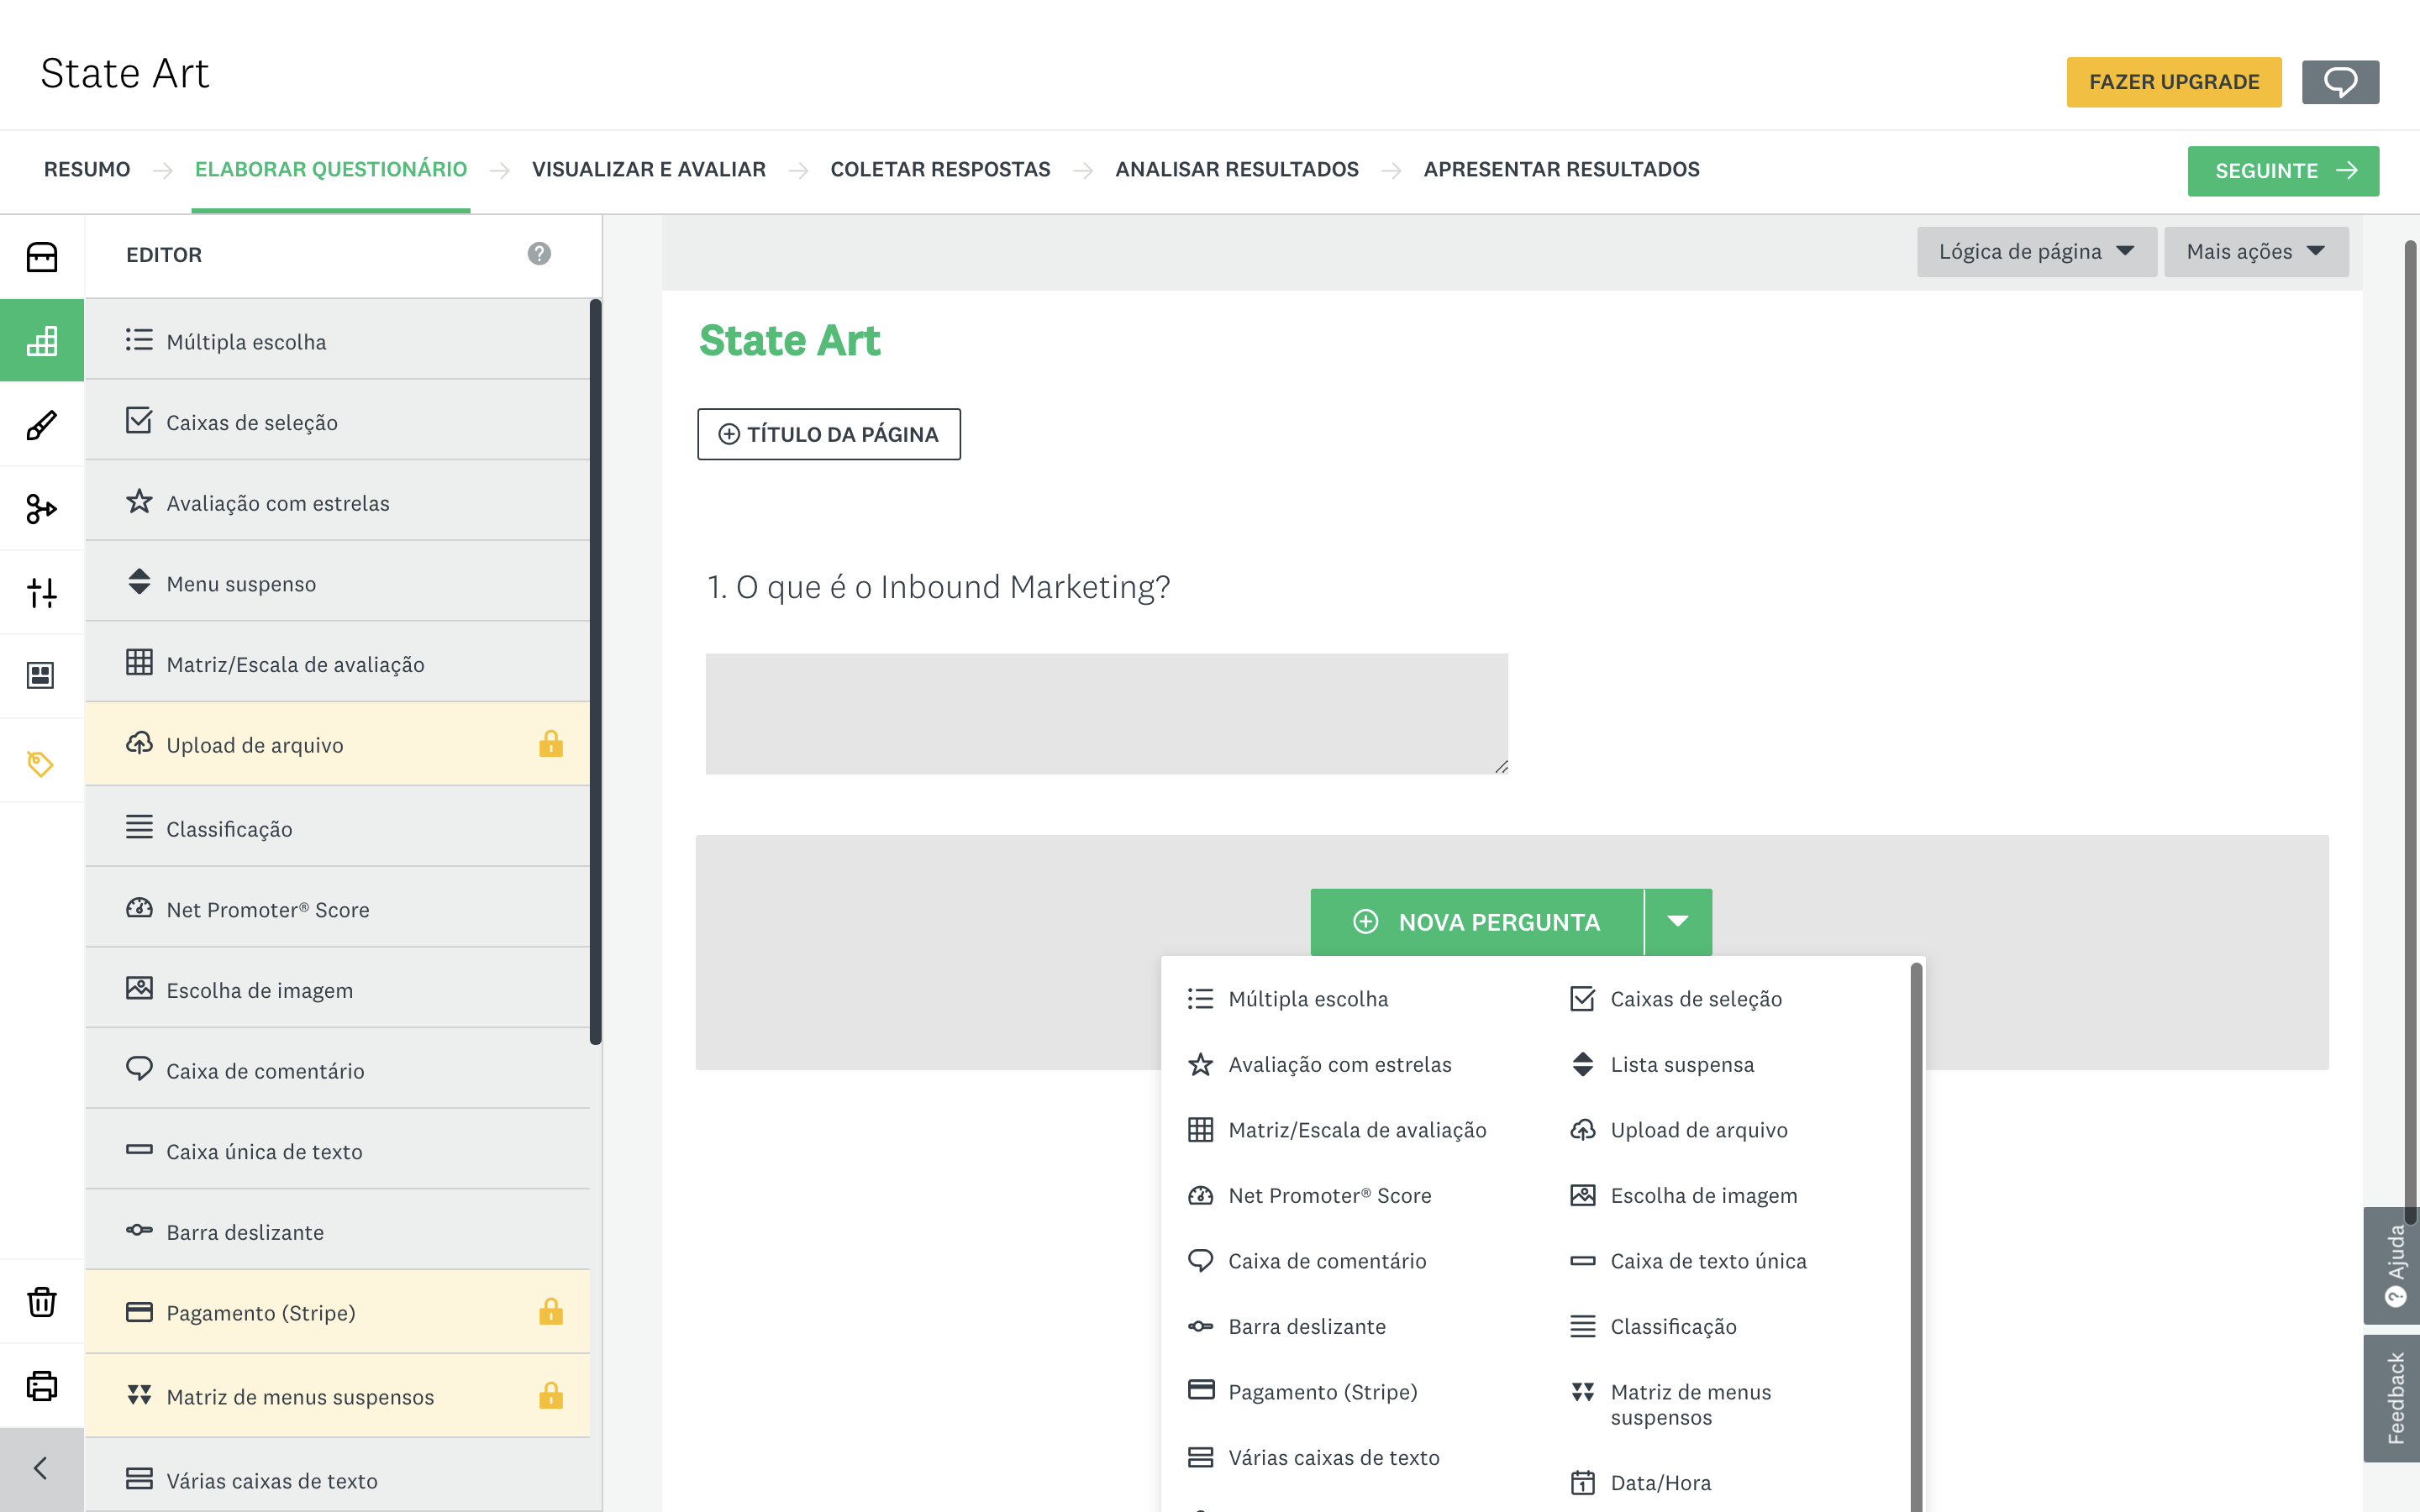
\includegraphics[width=1\textwidth]{img/sm/surveymonkey-form-element}
		\caption{SurveyMonkey - Elementos }
		\label{fig:surveymonkey-form-element}
	\end{center}
\end{figure}
\newpage

\begin{figure}[ht!]
	\begin{center}
		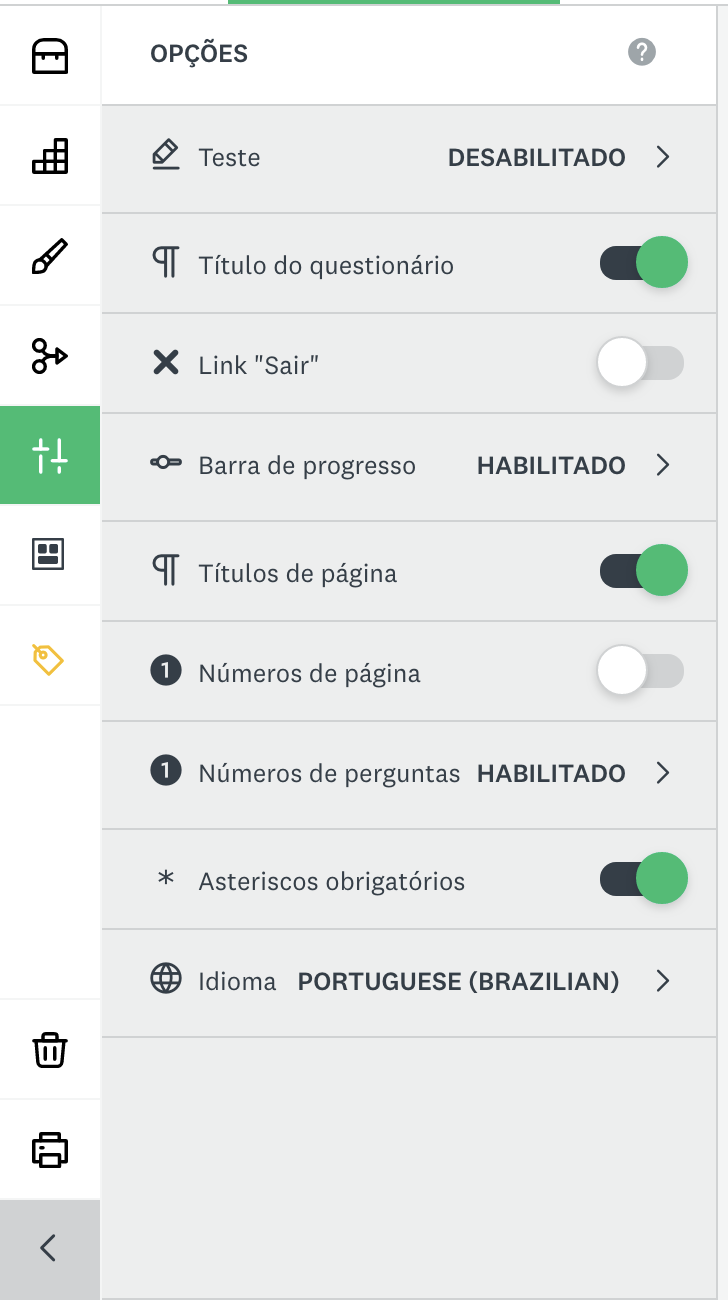
\includegraphics[height=.35\textheight]{img/sm/surveymonkey-form-opcoes}
		\caption{SurveyMonkey - Opções}
		\label{fig:surveymonkey-form-opcoes}
	\end{center}
\end{figure}

\begin{figure}[ht!]
	\begin{center}
		\begin{minipage}{0.45\textwidth}
			\begin{center}
				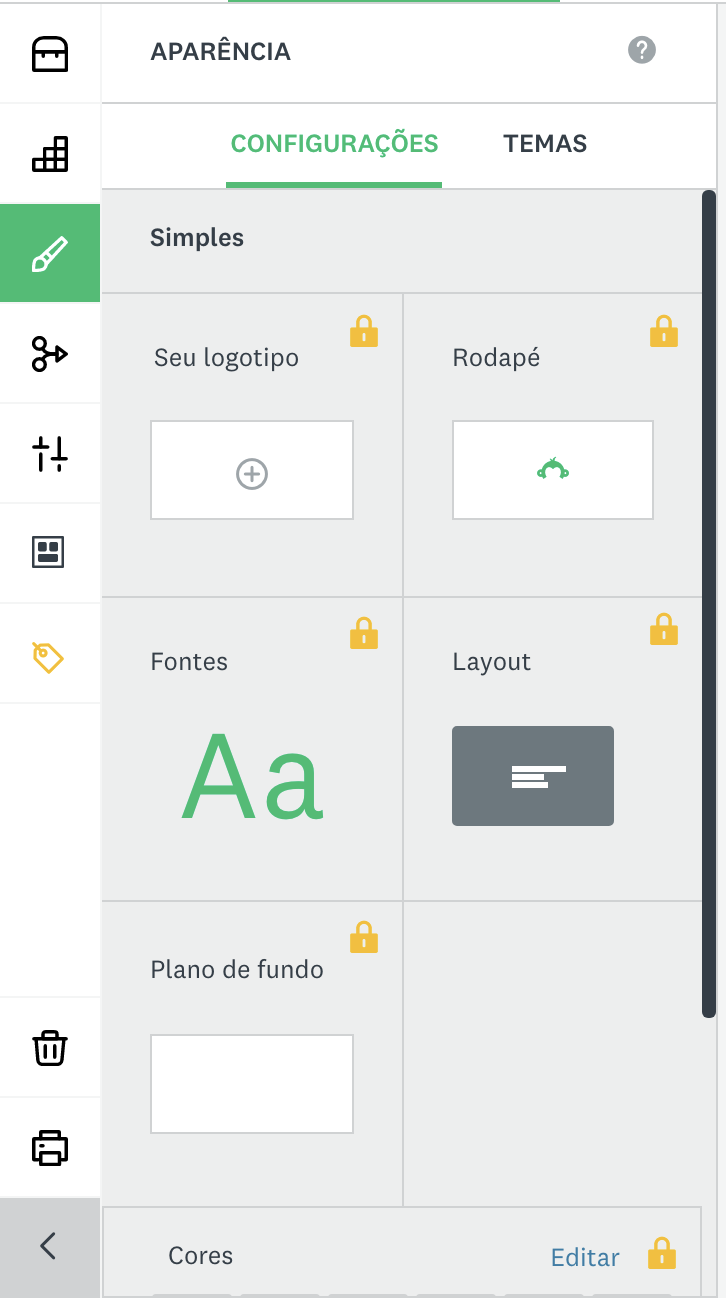
\includegraphics[height=.35\textheight]{img/sm/surveymonkey-form-aparencia}
				\caption{SurveyMonkey - Aparência}
				\label{fig:surveymonkey-form-aparencia}
			\end{center}
		\end{minipage}
		\hspace{1cm}
		\begin{minipage}{0.45\textwidth}
			\begin{center}
				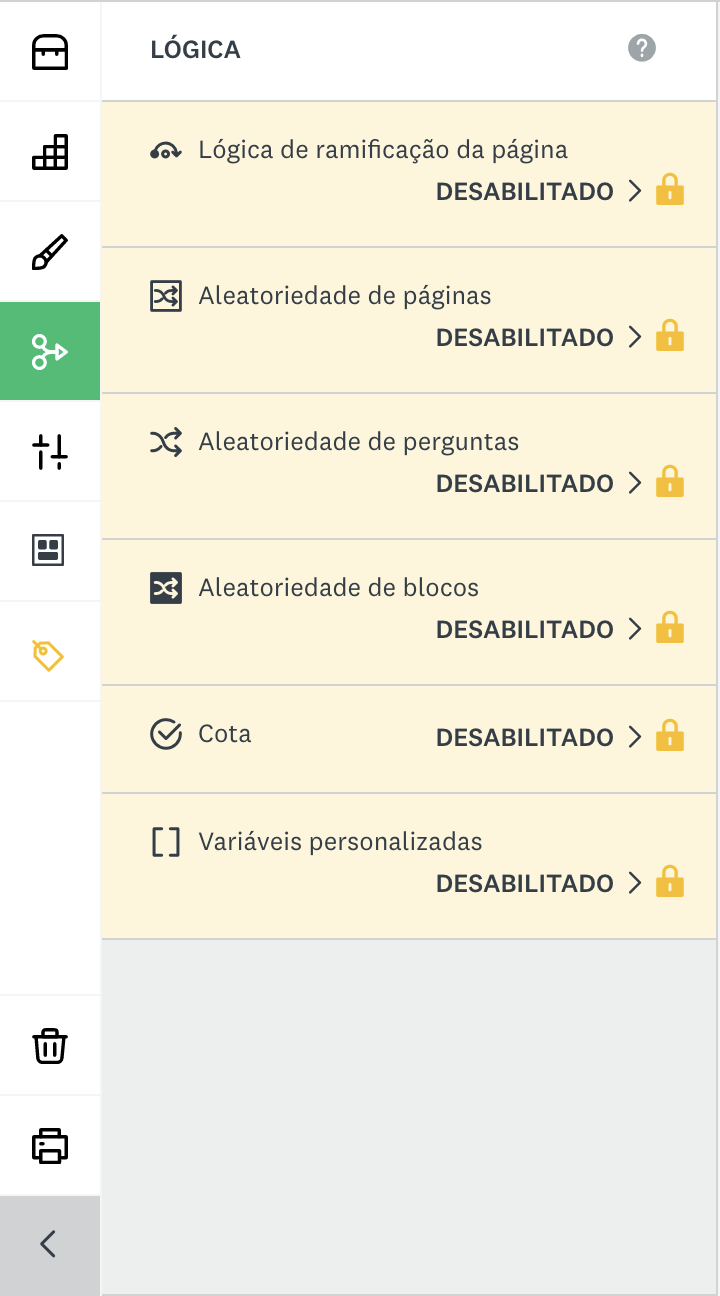
\includegraphics[height=.35\textheight]{img/sm/surveymonkey-form-logica}
				\caption{SurveyMonkey - Lógica}
				\label{fig:surveymonkey-form-logica}
			\end{center}
		\end{minipage}
	\end{center}
\end{figure}

O SurveyMonkey permite também realizar algumas operações de personalização do formulário.Na Figuras \ref{fig:surveymonkey-form-opcoes}, \ref{fig:surveymonkey-form-aparencia} e \ref{fig:surveymonkey-form-logica} estão representaçãs as opções, aparência e lógica do formulário, respetivamente, que permite costumizar formulários ao público alvo. 
Depois de realizado o formulário esta plataforma permite a visualização do mesmo, em diferentes tipos de dispositivos, como se pode ver nas Figuras \ref{fig:surveymonkey-form-test-pc} e \ref{fig:surveymonkey-form-test-phone}, para verificar se tudo está conforme planeado para se poder prosseguir para a recolha de dados. 
 \newpage

\begin{figure}[ht!]
	\begin{center}
		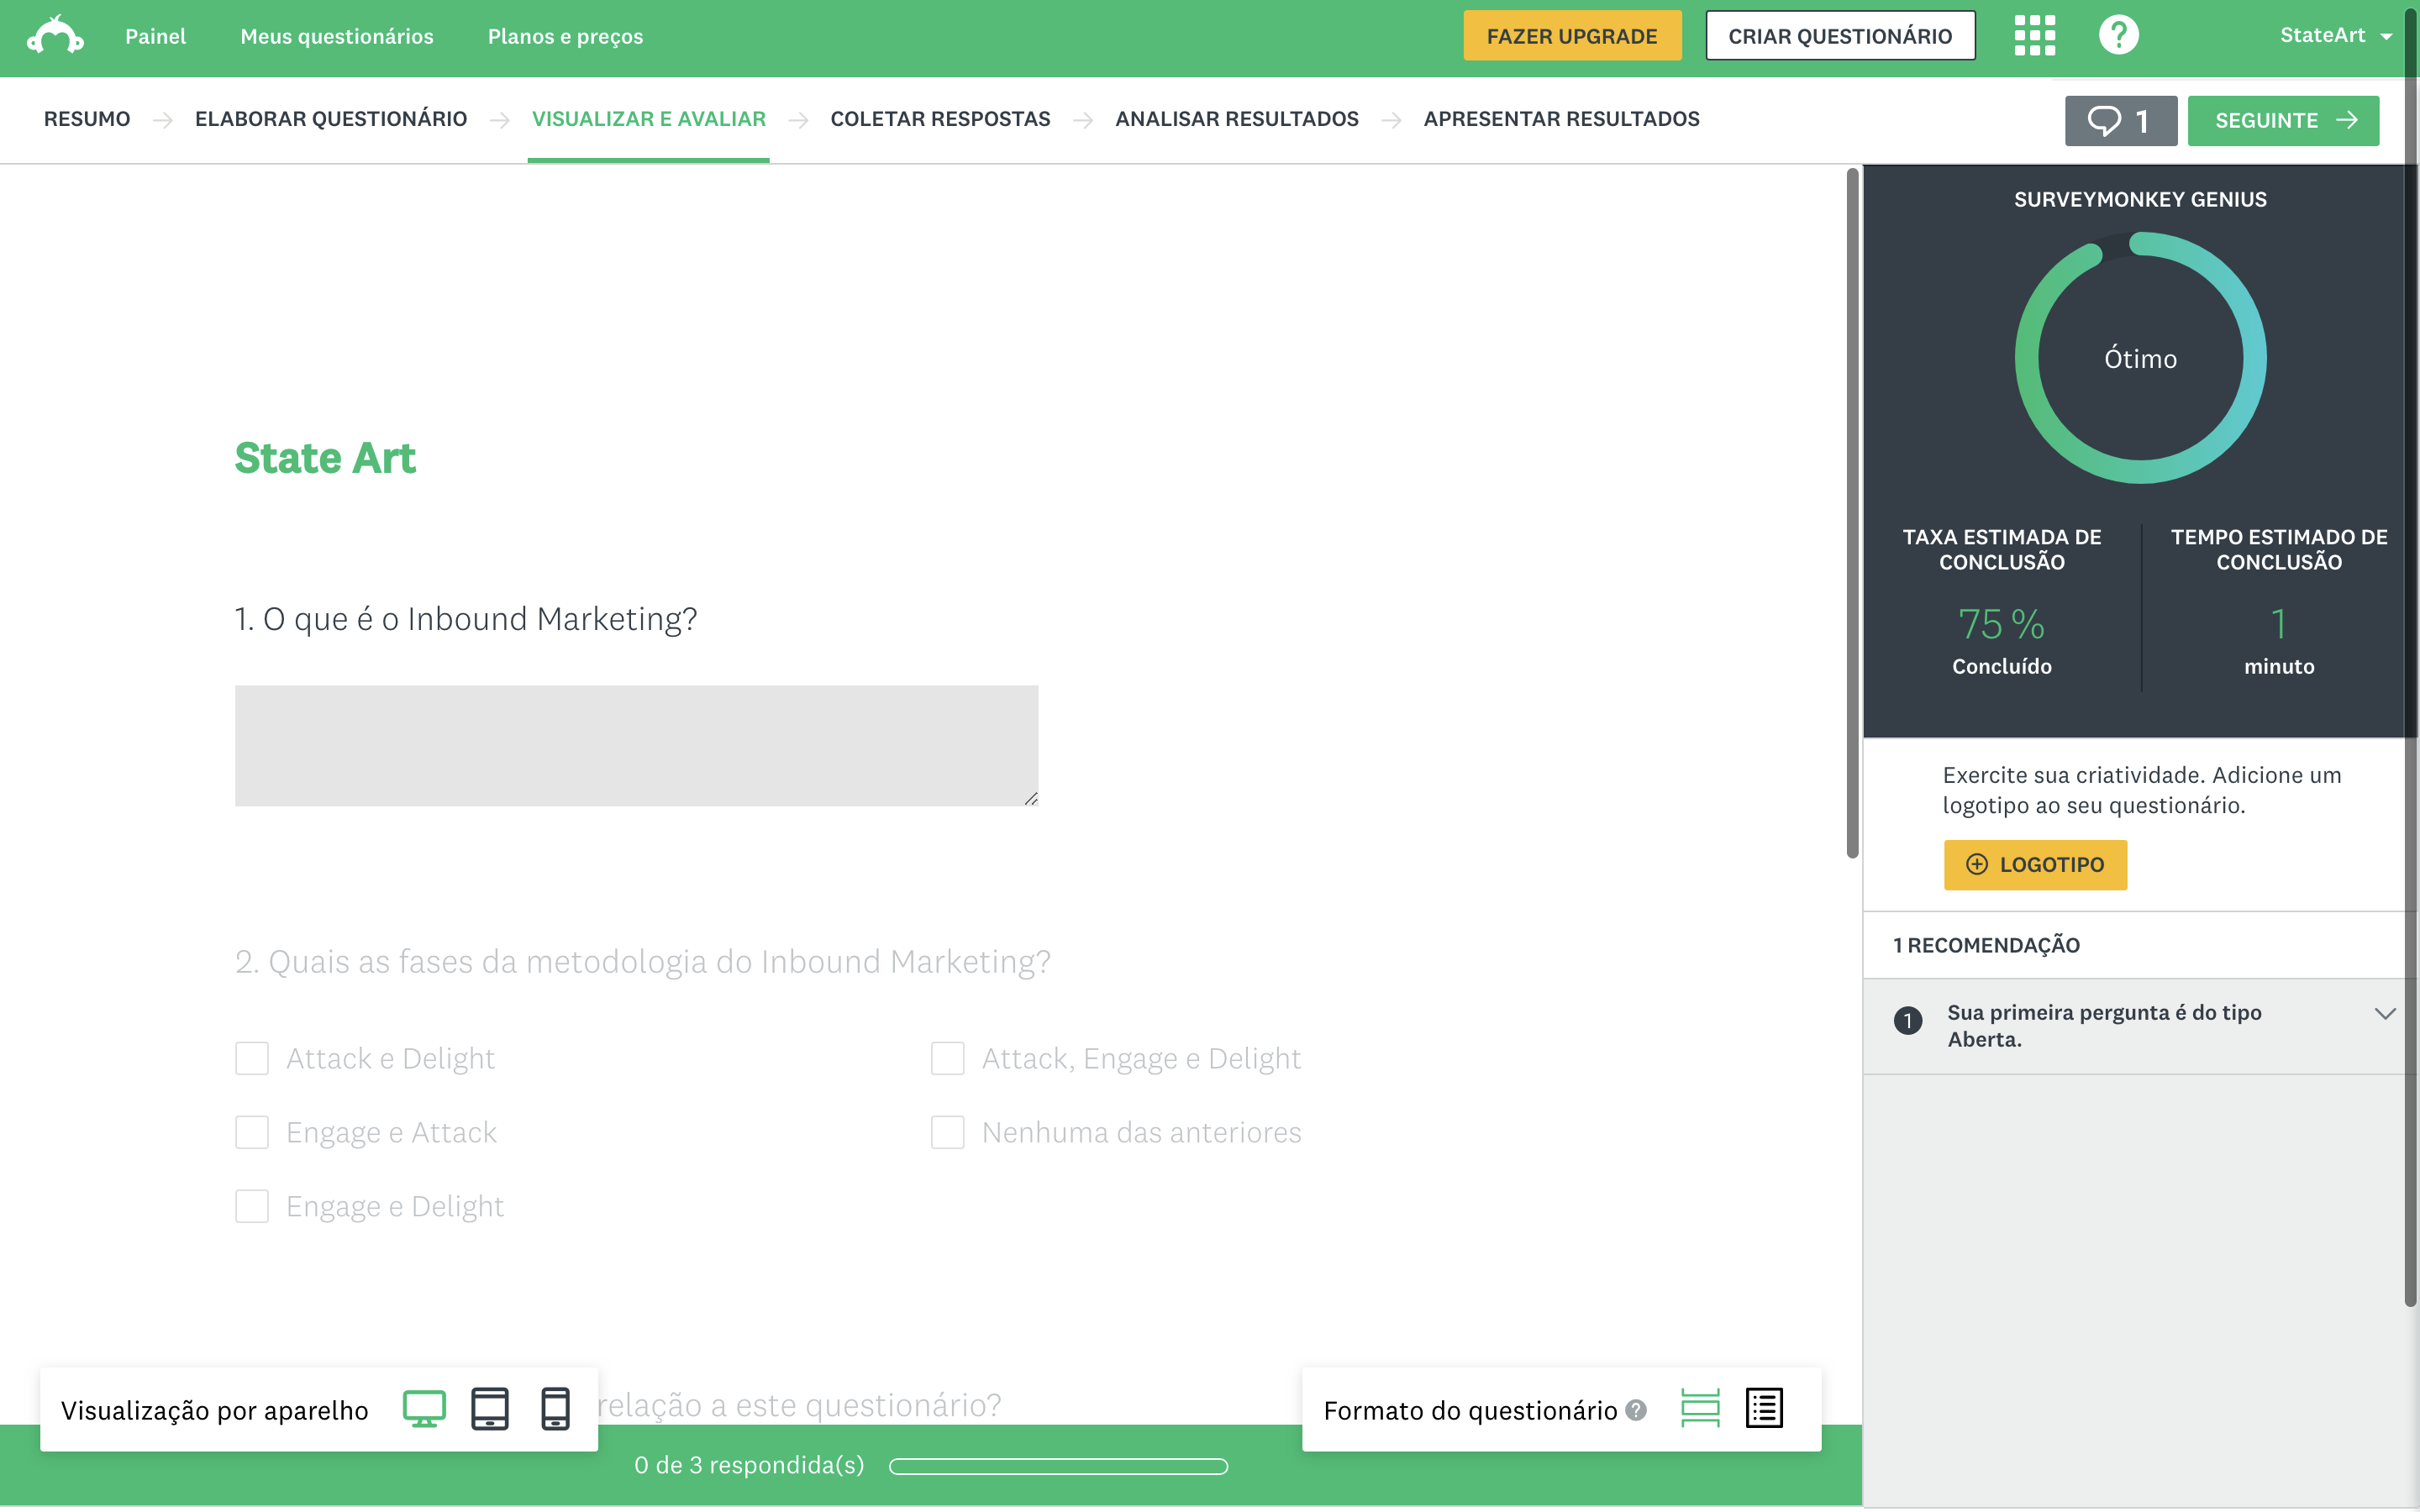
\includegraphics[width=1\textwidth]{img/sm/surveymonkey-form-test-pc}
		\caption{SurveyMonkey - Visualização do formulário em computador }
		\label{fig:surveymonkey-form-test-pc}
	\end{center}
\end{figure}

\begin{figure}[ht!]
	\begin{center}
		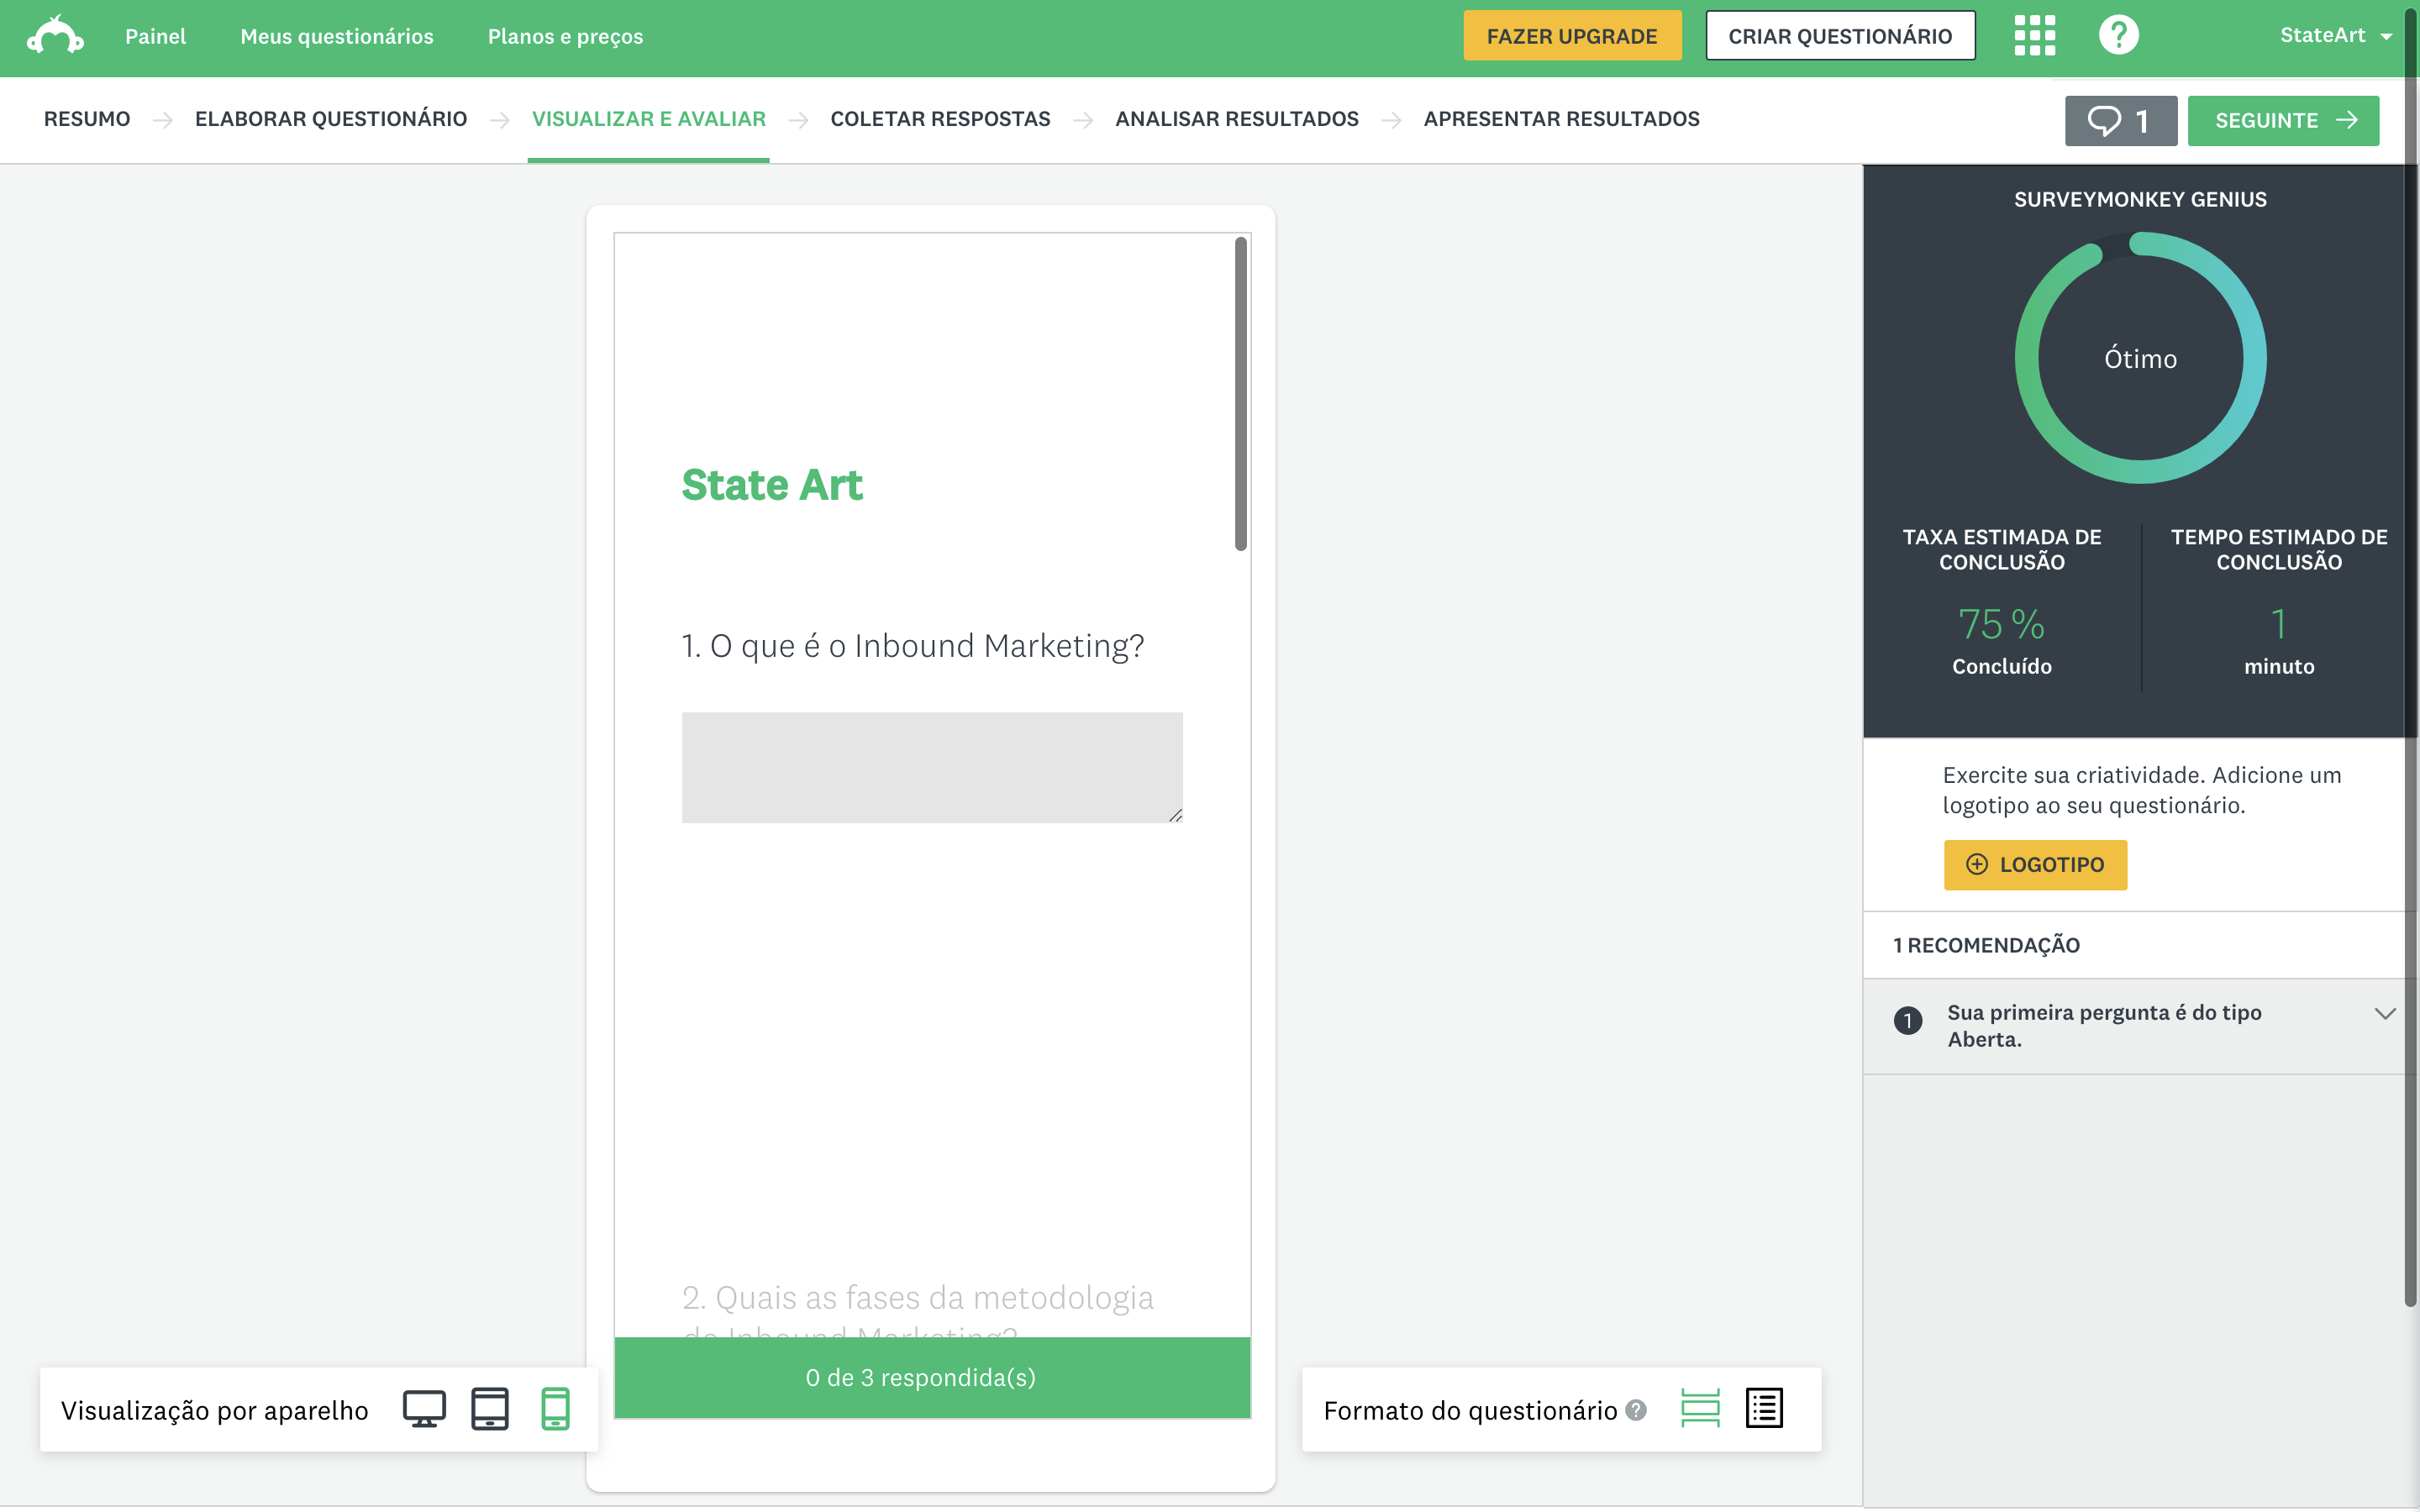
\includegraphics[width=1\textwidth]{img/sm/surveymonkey-form-test-phone}
		\caption{SurveyMonkey - Visualisação do formulário em smartphone }
		\label{fig:surveymonkey-form-test-phone}
	\end{center}
\end{figure}

Depois de garantir que o formulário foi construido como desejado a plataforma fornece vários meios pelo qual se pode partilhar/enviar o formulário, como listado na Figura \ref{fig:surveymonkey-form-share}.

\newpage

\begin{figure}[ht!]
	\begin{center}
		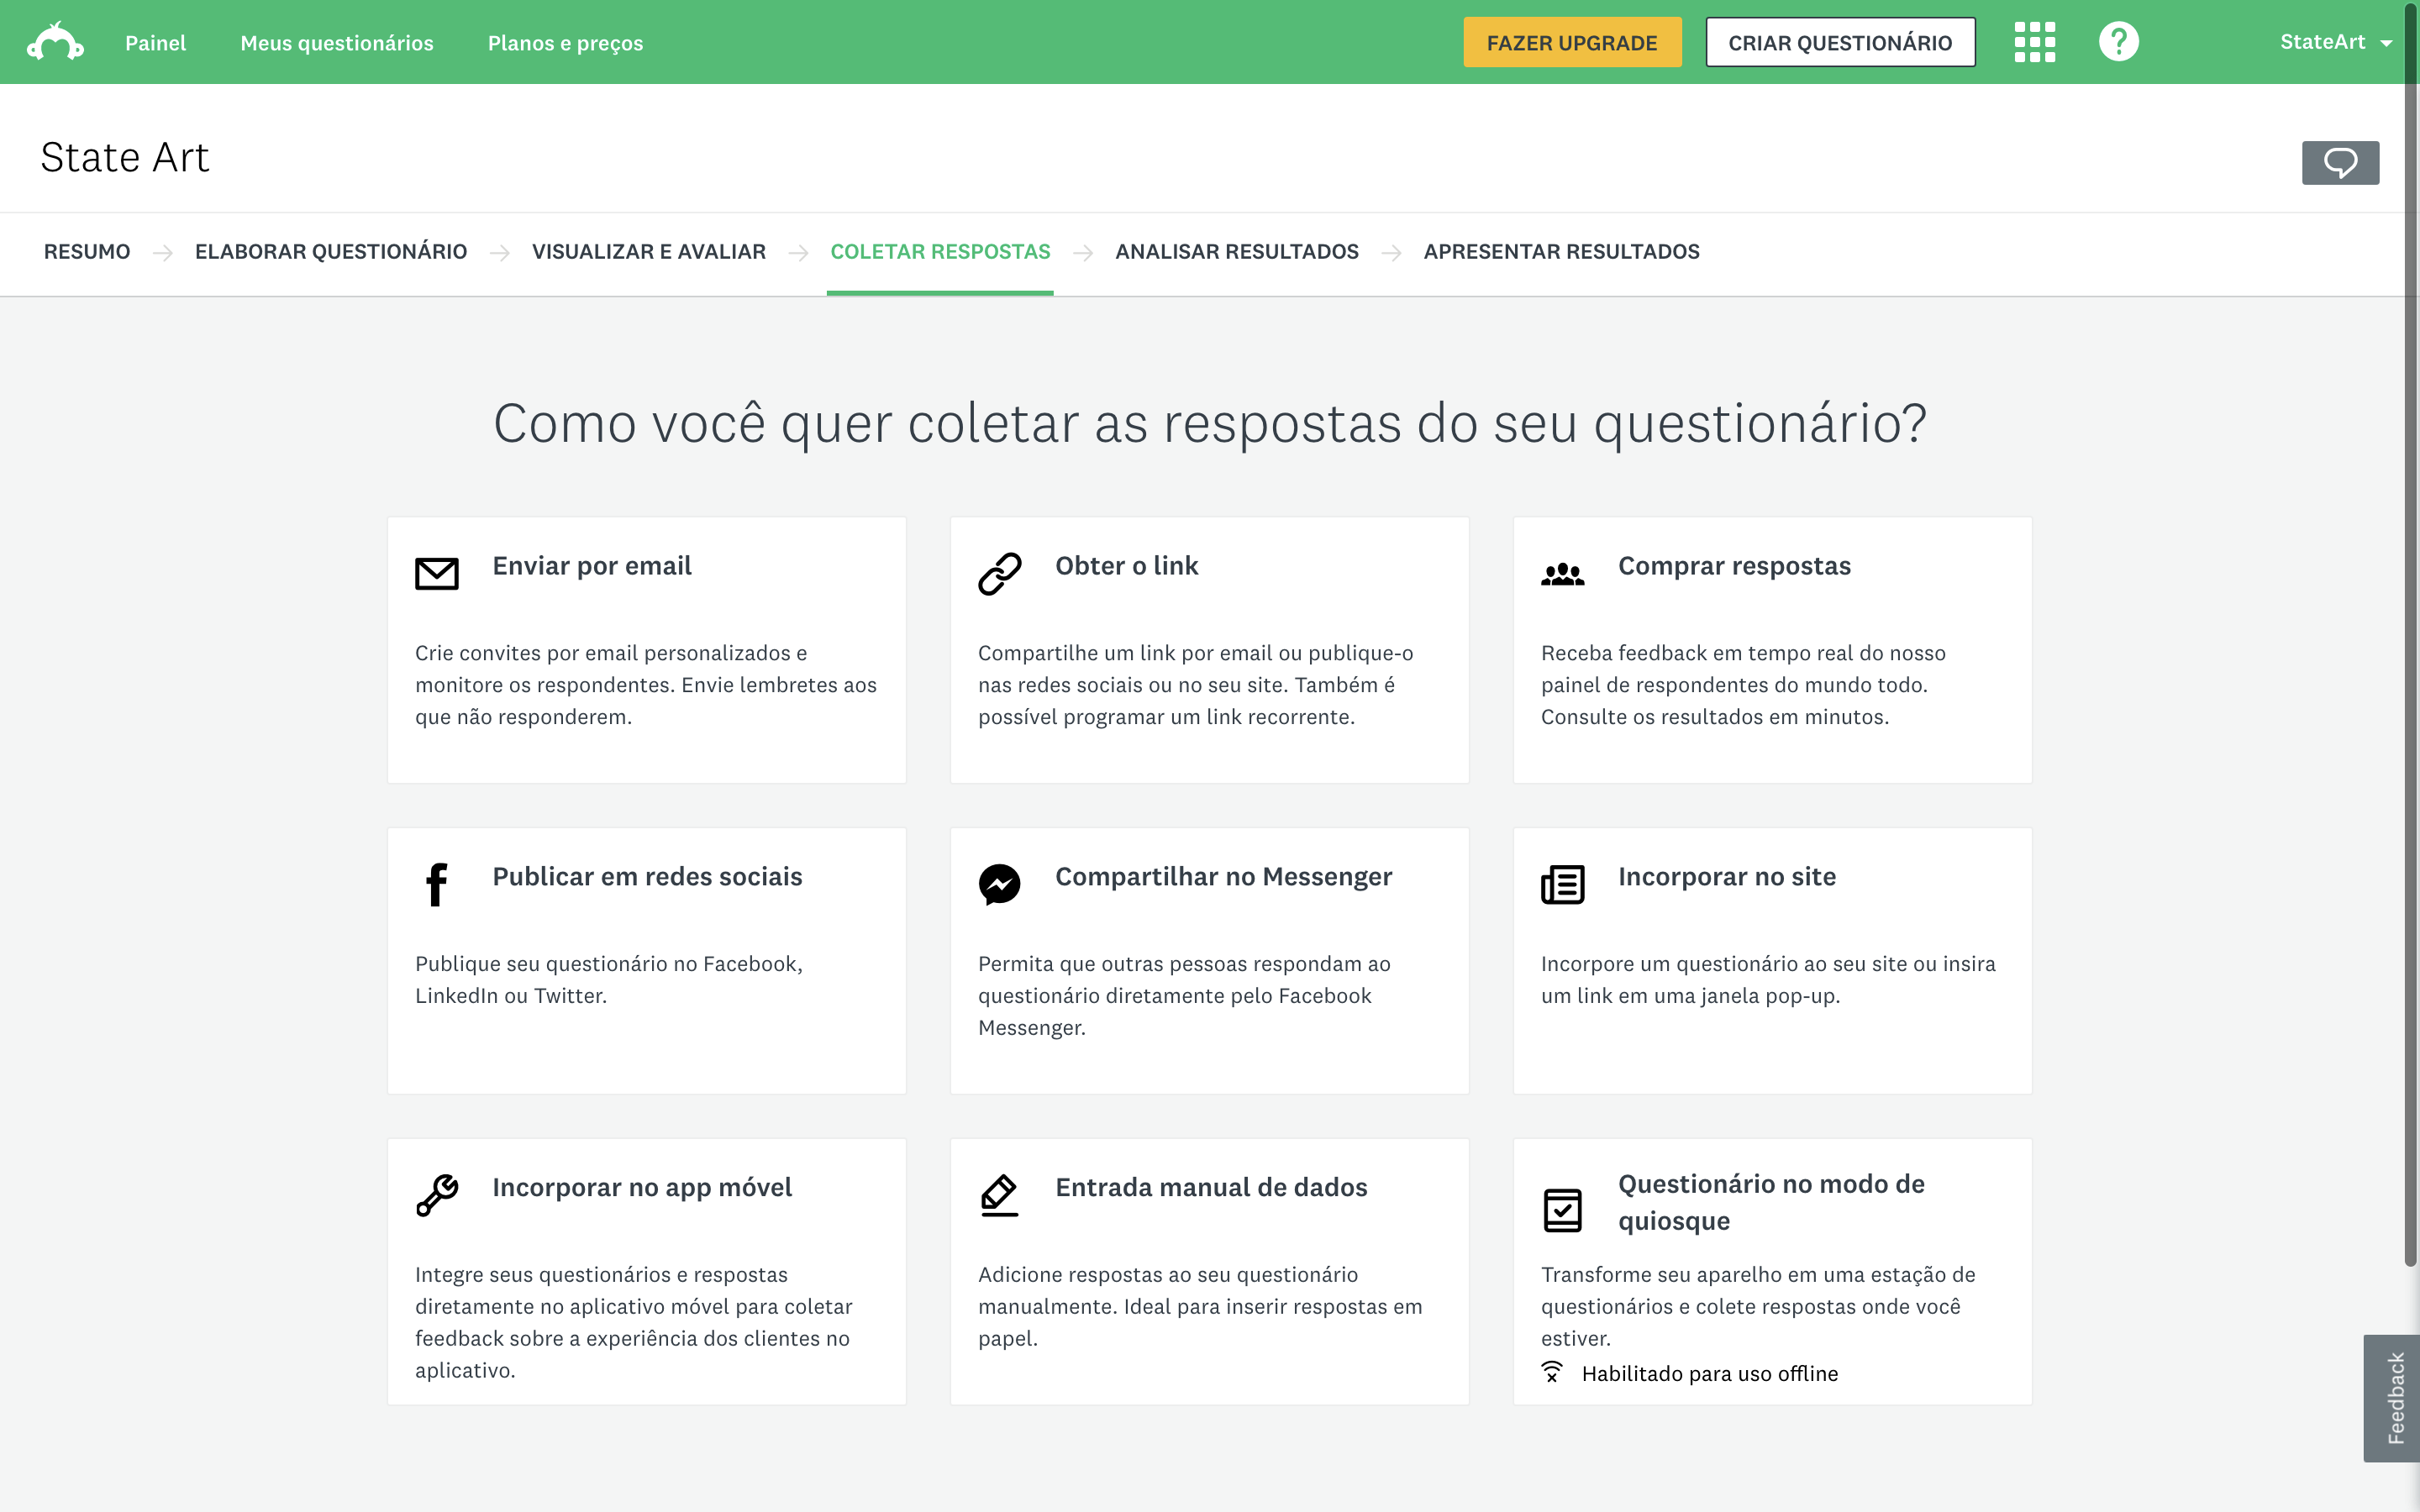
\includegraphics[width=1\textwidth]{img/sm/surveymonkey-form-share}
		\caption{SurveyMonkey - Metodo de partilha do formulário }
		\label{fig:surveymonkey-form-share}
	\end{center}
\end{figure}

Na analise de resultados, é necessário actualizar a página ou aplicar um filtro para que os gráficos e as estatísticas sejam actualizadas. 
O mesmo se passa na página que pode ser gerada para partilhar o sumário dos dados recolhidos, através do formulário. 
Para aplicar um filtro é necessário escolher o tipo de filtro e os elementos ao qual queremos aplicar o filtro como podemos ver nas Figuras \ref{fig:surveymonkey-form-filtro} e \ref{fig:surveymonkey-form-filtro1}. 


\begin{figure}[ht!]
	\begin{center}
		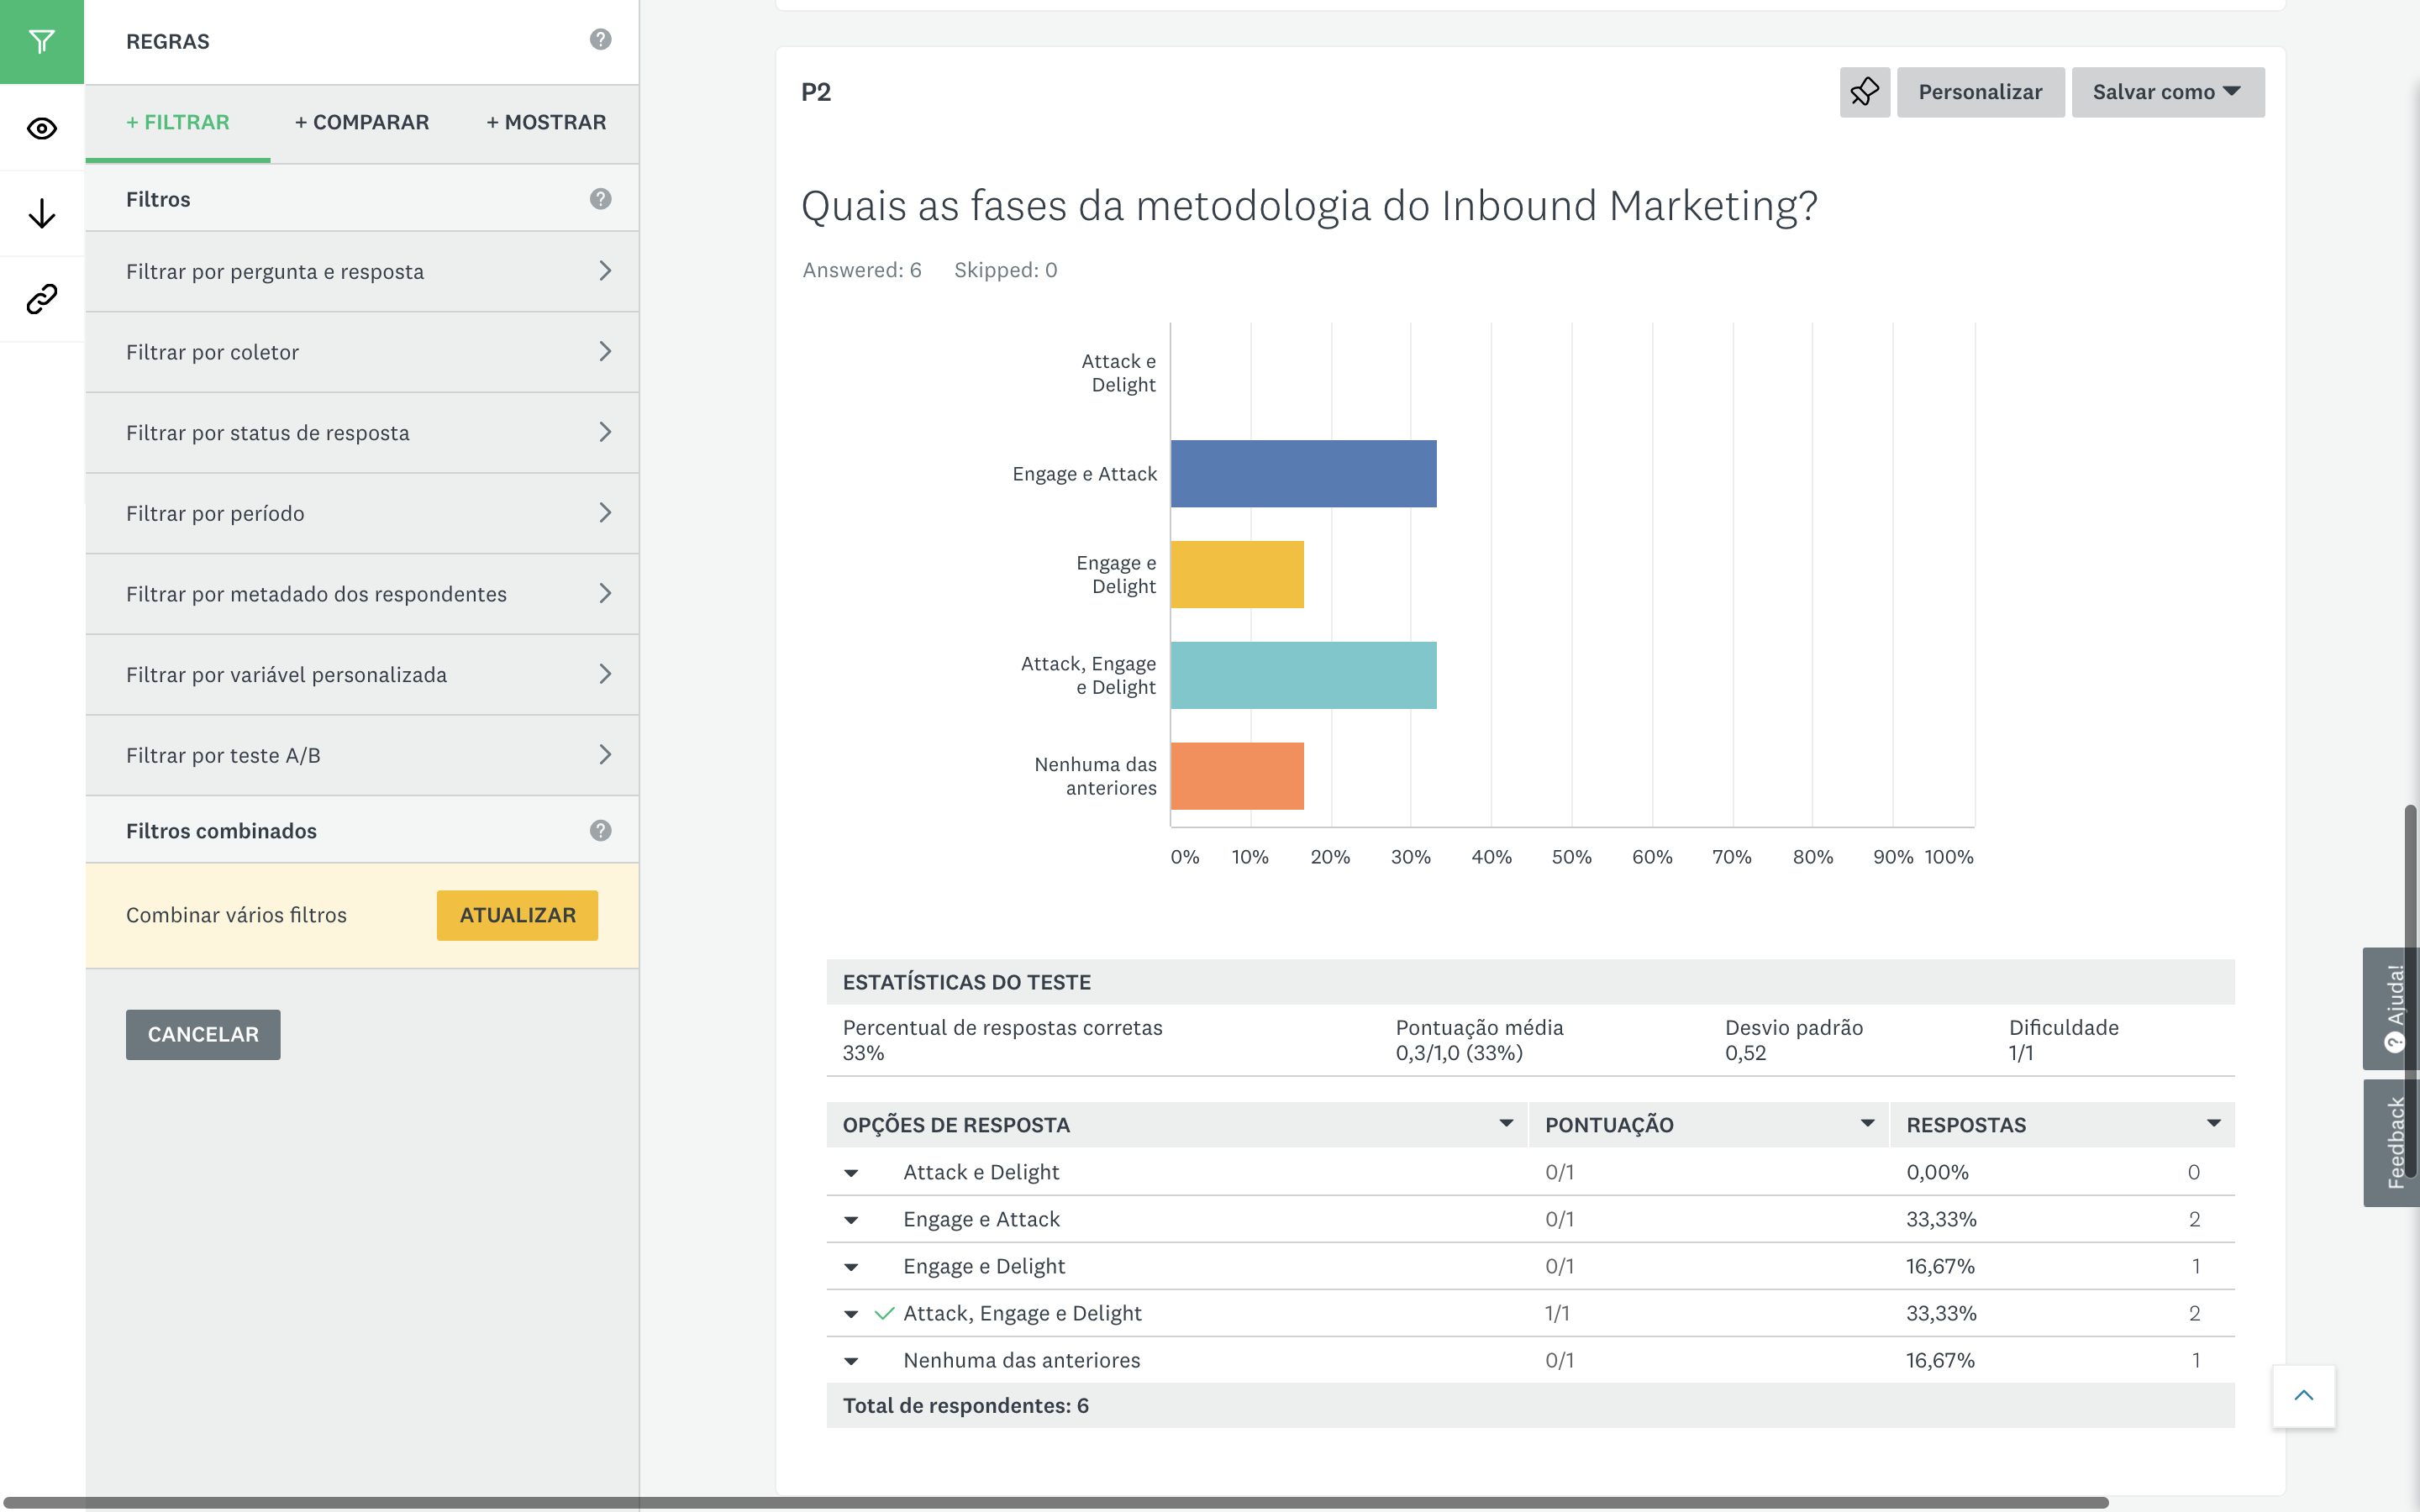
\includegraphics[width=1\textwidth]{img/sm/surveymonkey-form-filtro}
		\caption{SurveyMonkey - Tipos de Filtros }
		\label{fig:surveymonkey-form-filtro}
	\end{center}
\end{figure}



\begin{figure}[ht!]
	\begin{center}
		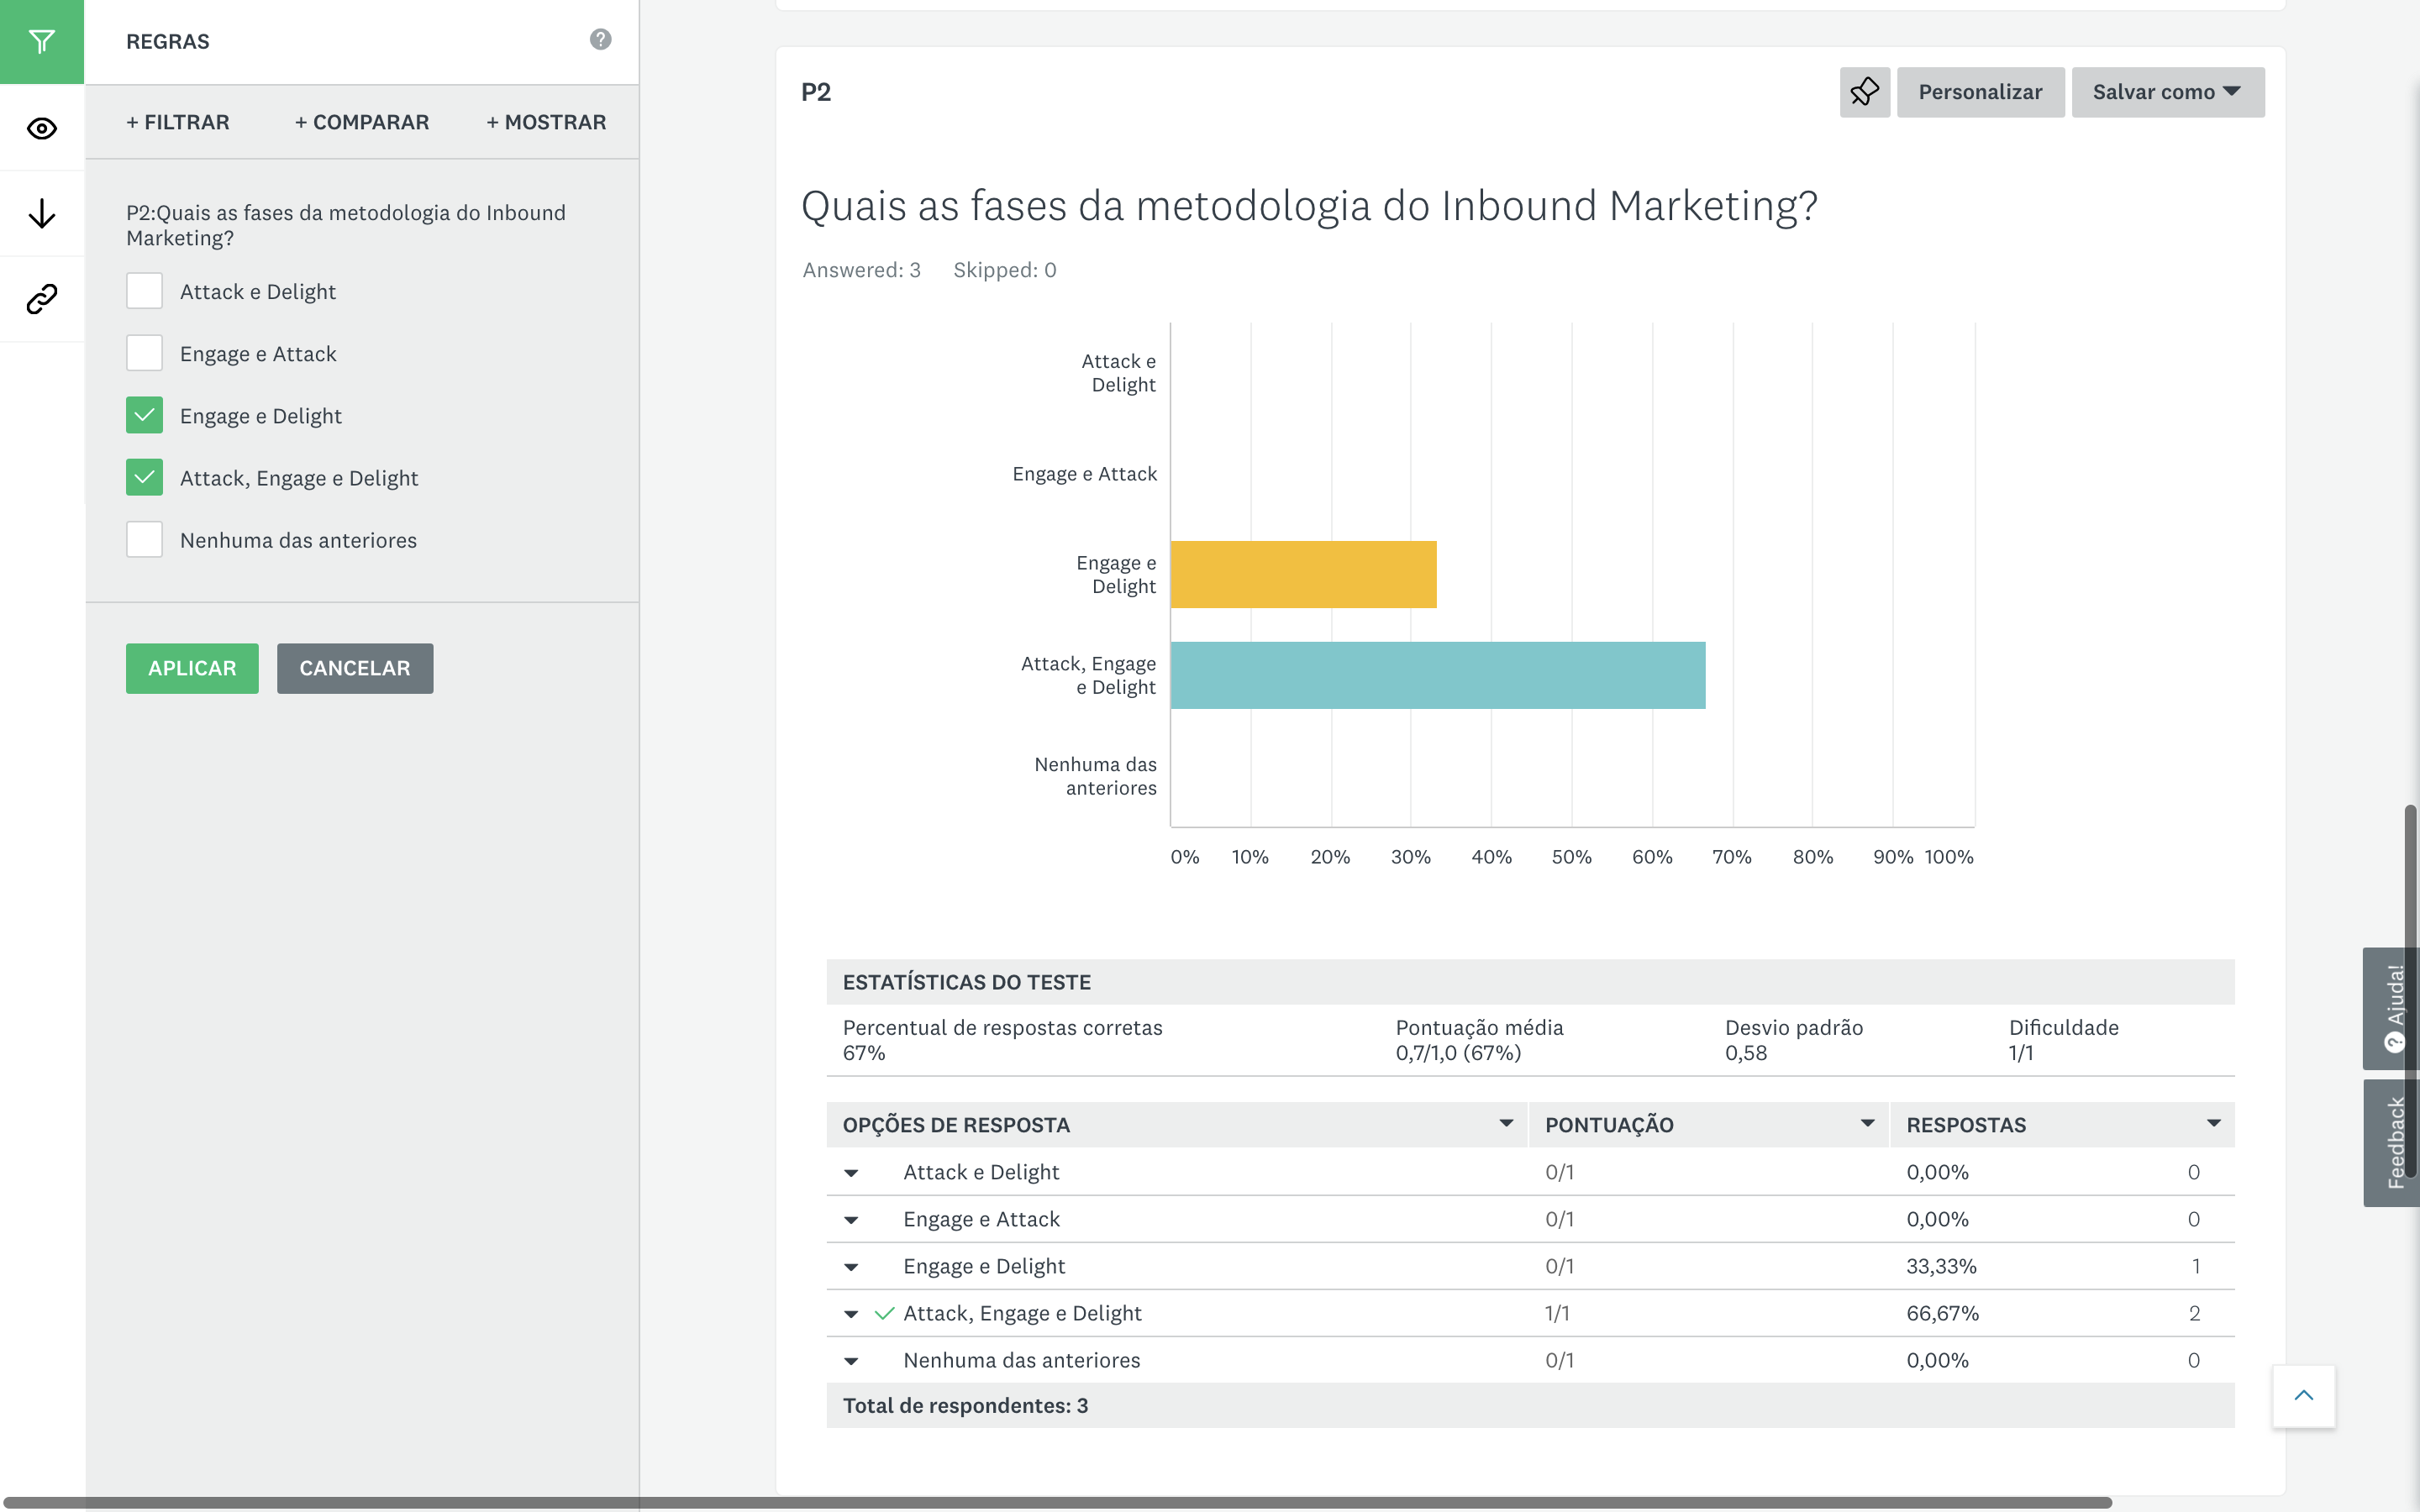
\includegraphics[width=1\textwidth]{img/sm/surveymonkey-form-filtro1}
		\caption{SurveyMonkey - Filtro aplicado na pergunta 2 }
		\label{fig:surveymonkey-form-filtro1}
	\end{center}
\end{figure}

\newpage



Para finalizar a plataforma SurveyMonkey tem ainda uma funcionalidade que, através da representação dos dados numa linha temporal, permite o utilizador perceber as tendências dos dados.

\section{Typeform}
\label{typeform}

O Typeform é uma plataforma \acrshort{saas} de criação de formulários online. É uma empresa que afirma resolver o problema dos formulários e inquéritos aborrecidos e tem também como proposta de valor o facto de conseguir criar formulários e inquéritos sem ter que programar uma única linhad e código. Esta plataforma permite recolher informações do público alvo através de formulários e inquéritos personalizados e no final visualizar estes dados. 

O Typeform disponilibilisa um pacote gratuito, contudo, é necessário criar conta de utilizador, para aceder ás funcionalidades da plataforma. Tanto o registro como o início de sessão pode ser feito através da \acrfull{api} do Google.

Como podemos ver na Figura \ref{fig:tf-dashboard}, no painel de controlo, podemos criar várias áreas de trabalho. Cada área de trabalho é independente e todos os formulários e inquéritos que forem adicionados ao mesmo podem ser partilhados com mais do que uma pessoa.
\newpage

\begin{figure}[ht!]
	\begin{center}
		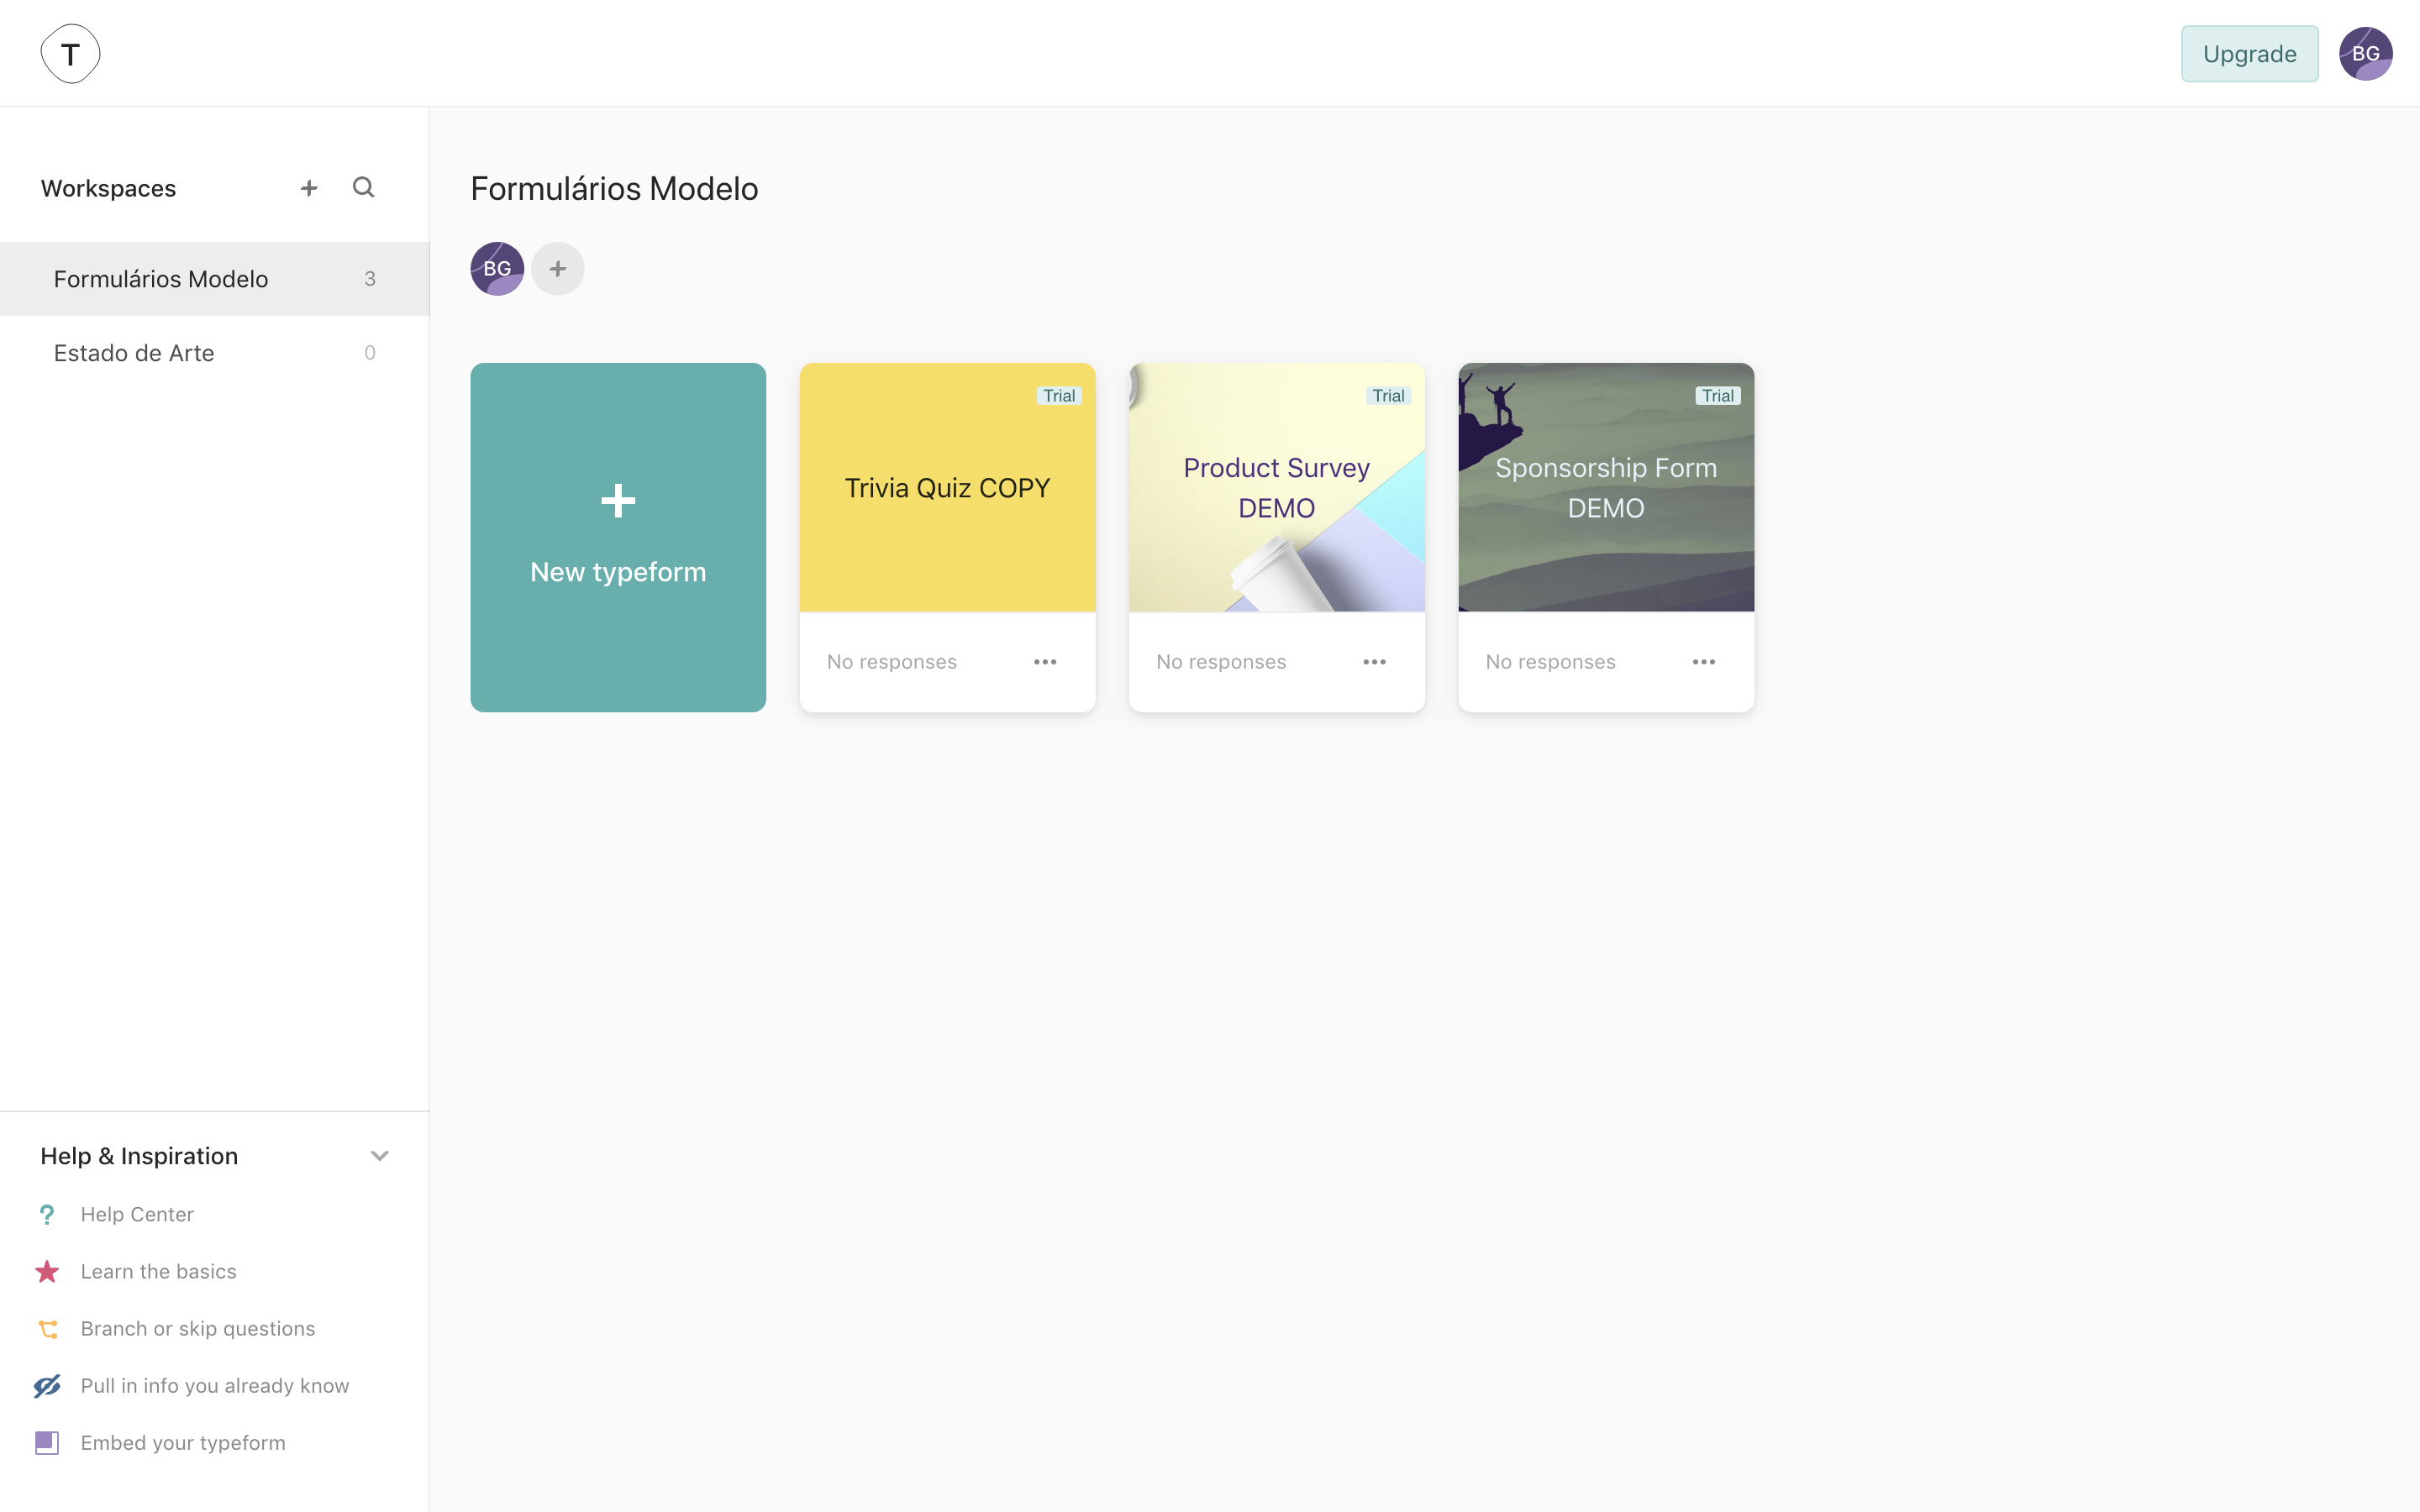
\includegraphics[width=1\textwidth]{img/tf/tf-dashboard}
		\caption{Typeform - Painel de Controlo}
		\label{fig:tf-dashboard}
	\end{center}
\end{figure}

Na criação de um formulário ou inquérito, do zero, a plataforma lista uma séria de templates que se podem filtrar por categorias na coluna à esquerda, como se pode observar na Figura \ref{fig:tf-form-create}.

\begin{figure}[ht!]
	\begin{center}
		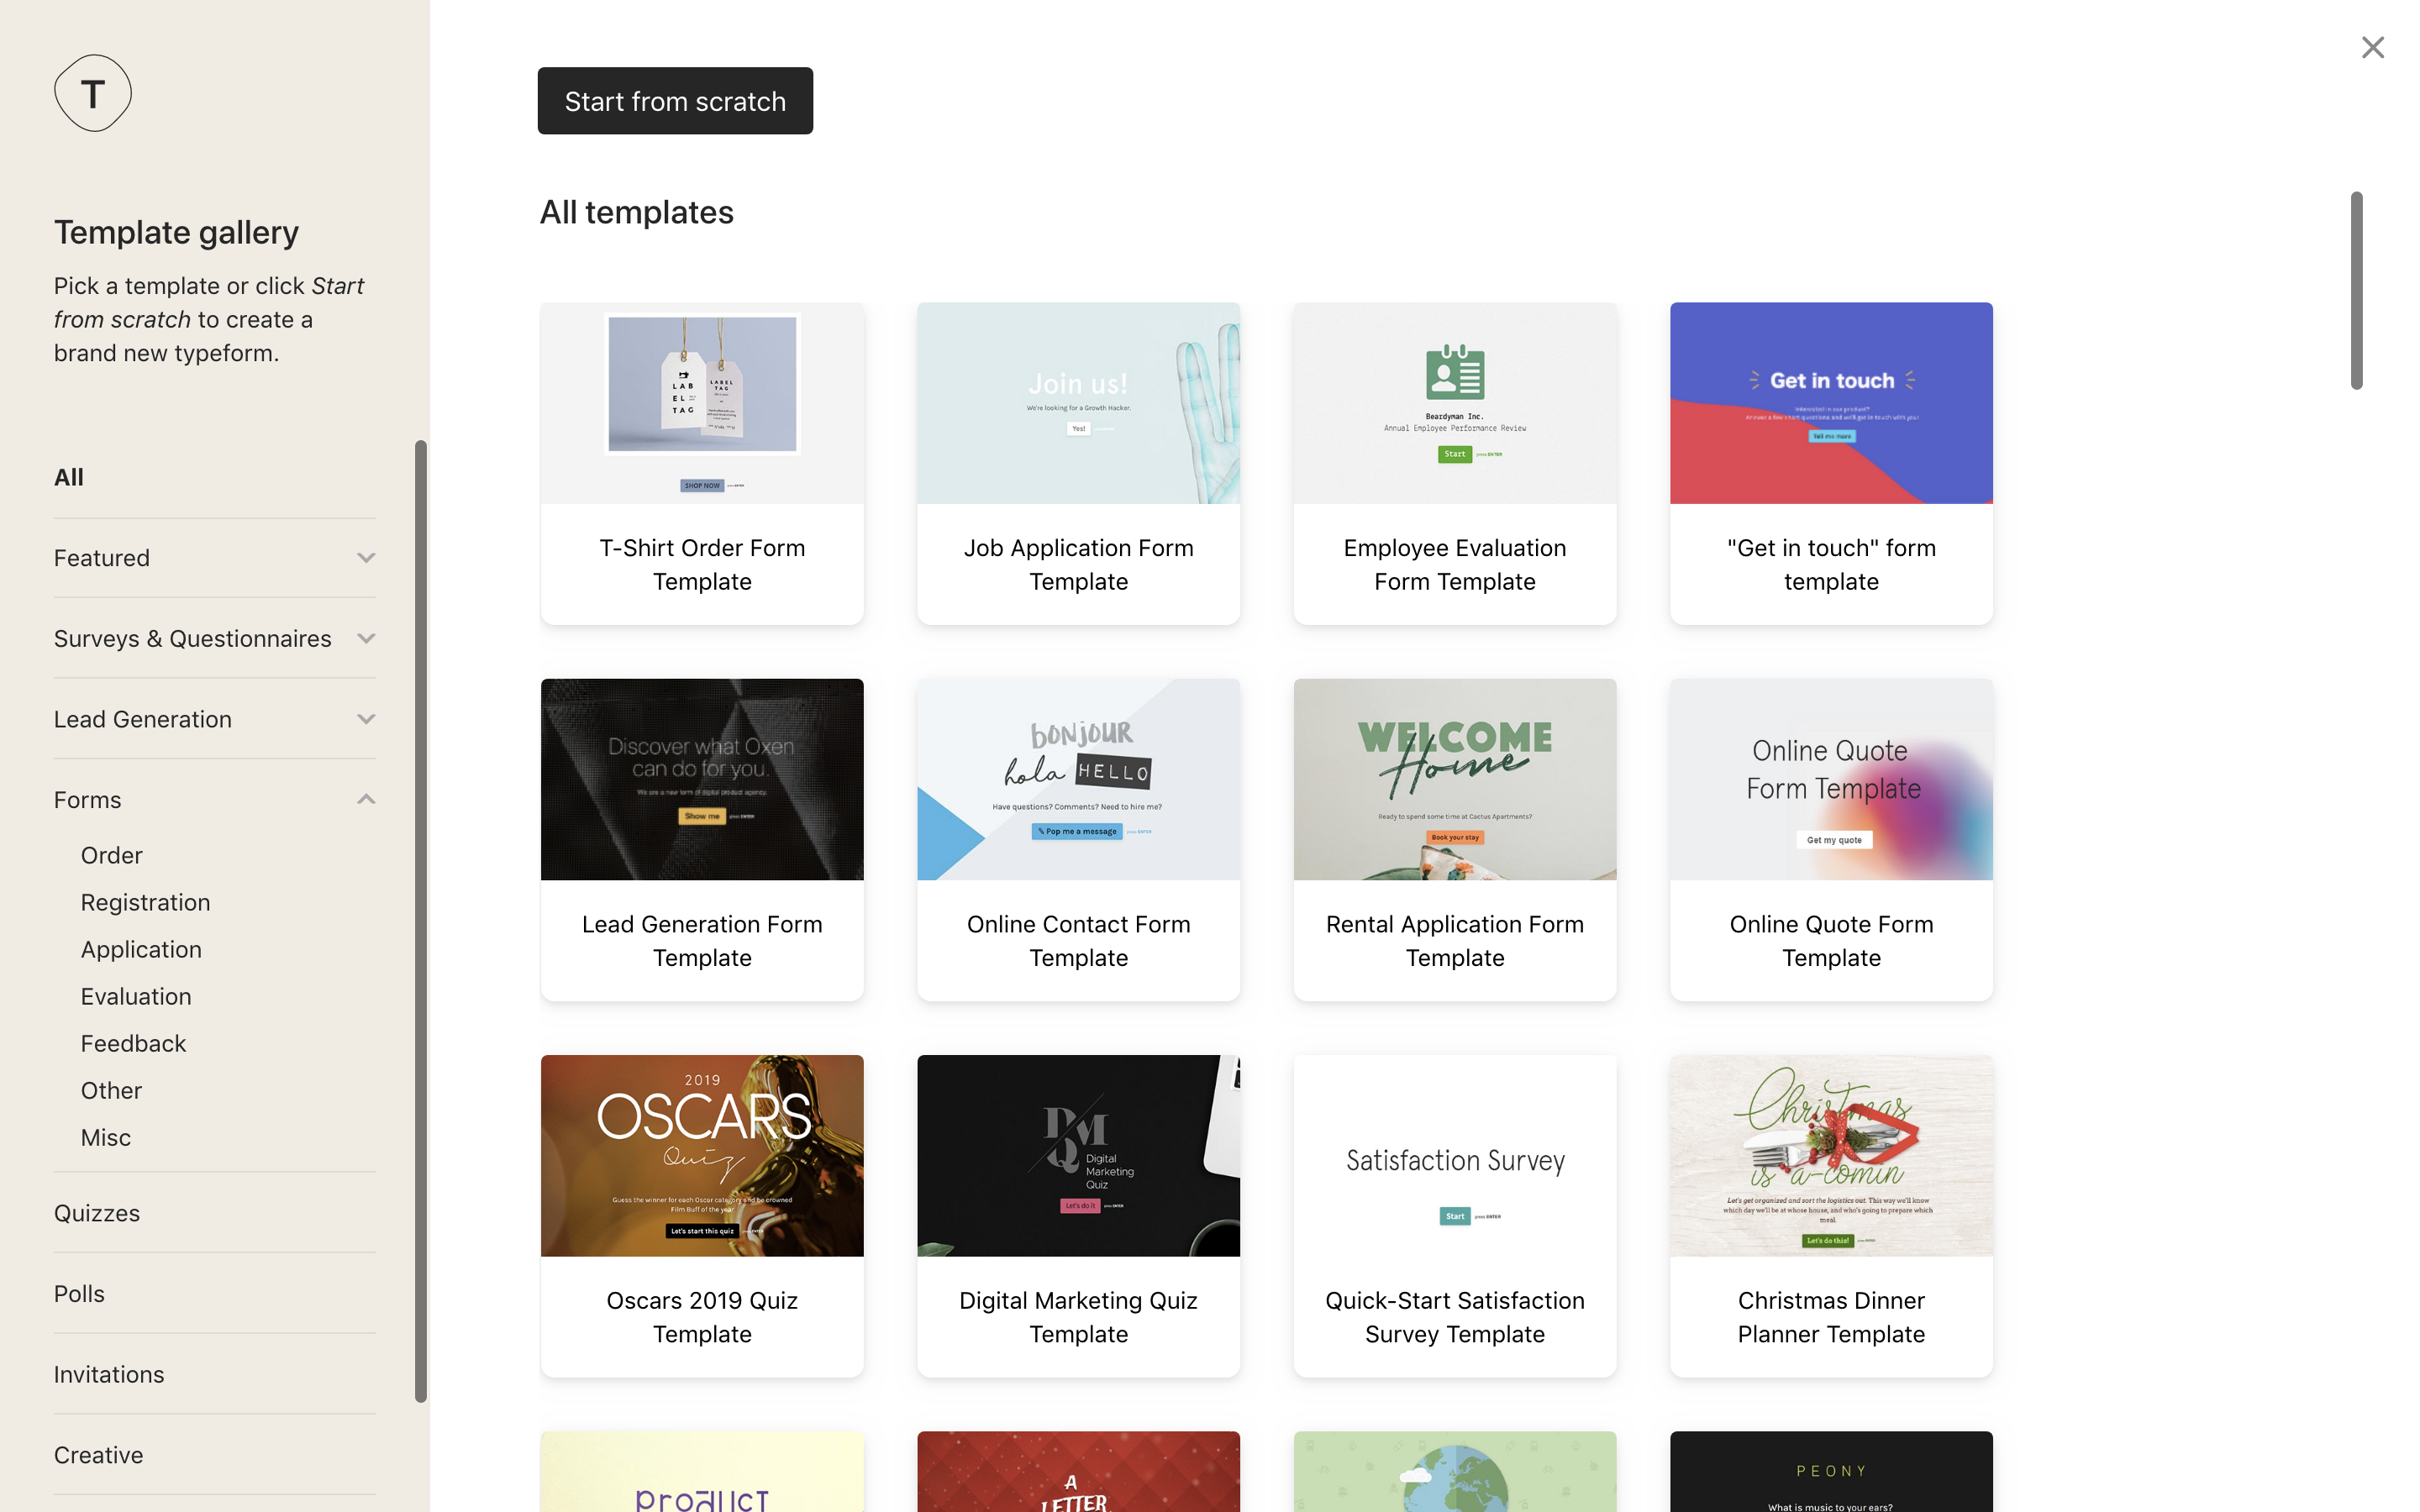
\includegraphics[width=1\textwidth]{img/tf/tf-form-create}
		\caption{Typeform - Criar Formulário}
		\label{fig:tf-form-create}
	\end{center}
\end{figure}
\newpage

\begin{figure}[ht!]
	\begin{center}
		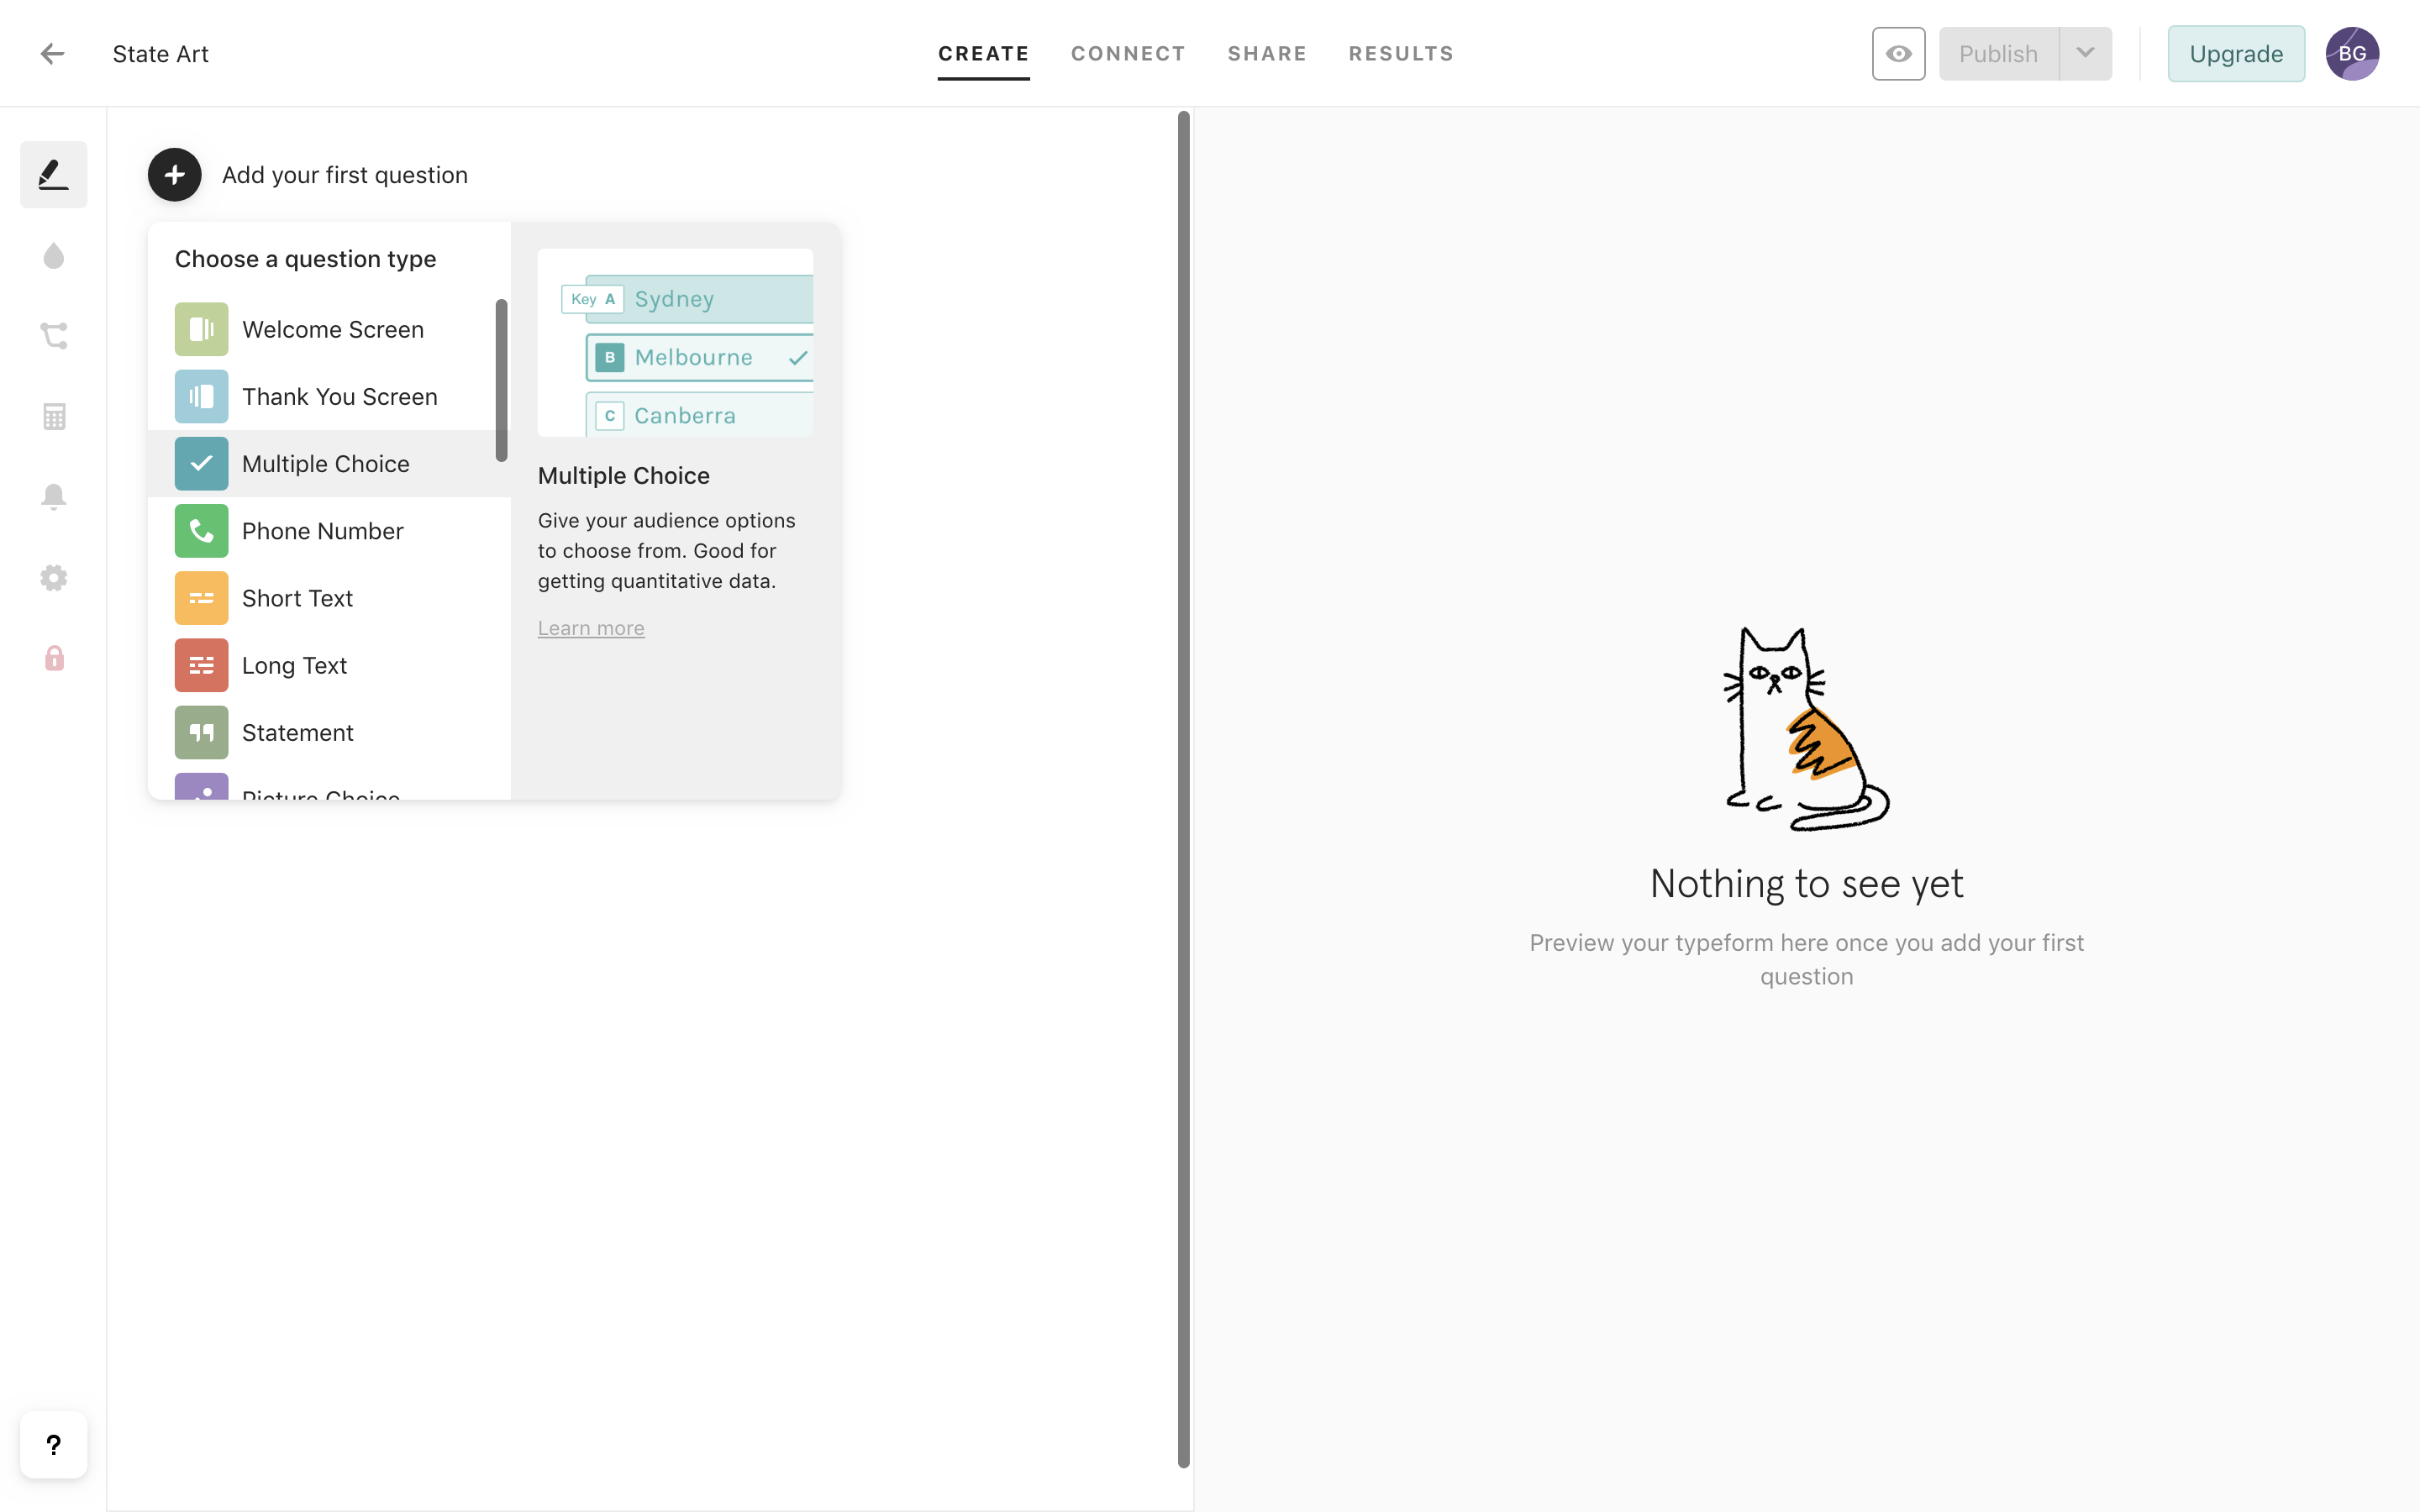
\includegraphics[width=1\textwidth]{img/tf/tf-question-type}
		\caption{Typeform - Tipos de pergunta}
		\label{fig:tf-question-type}
	\end{center}
\end{figure}

Representado na Figura \ref{fig:tf-question-type} temos os tipos de pergunta que a plataforma permite adicionar no formulário. Estas perguntas podem ser personalizaveis tanto a nível estético como funcional como podemos ver nas Figuras \ref{fig:tf-question-opcoes} e \ref{fig:tf-question-custom}, respectivamente. É também possível criar um tema novo para cada pergunta onde se pode escolher a fonte de texto, imagem de fundo e cores da pergunta, respostas, butões e fundo.

\begin{figure}[ht!]
	\begin{center}
		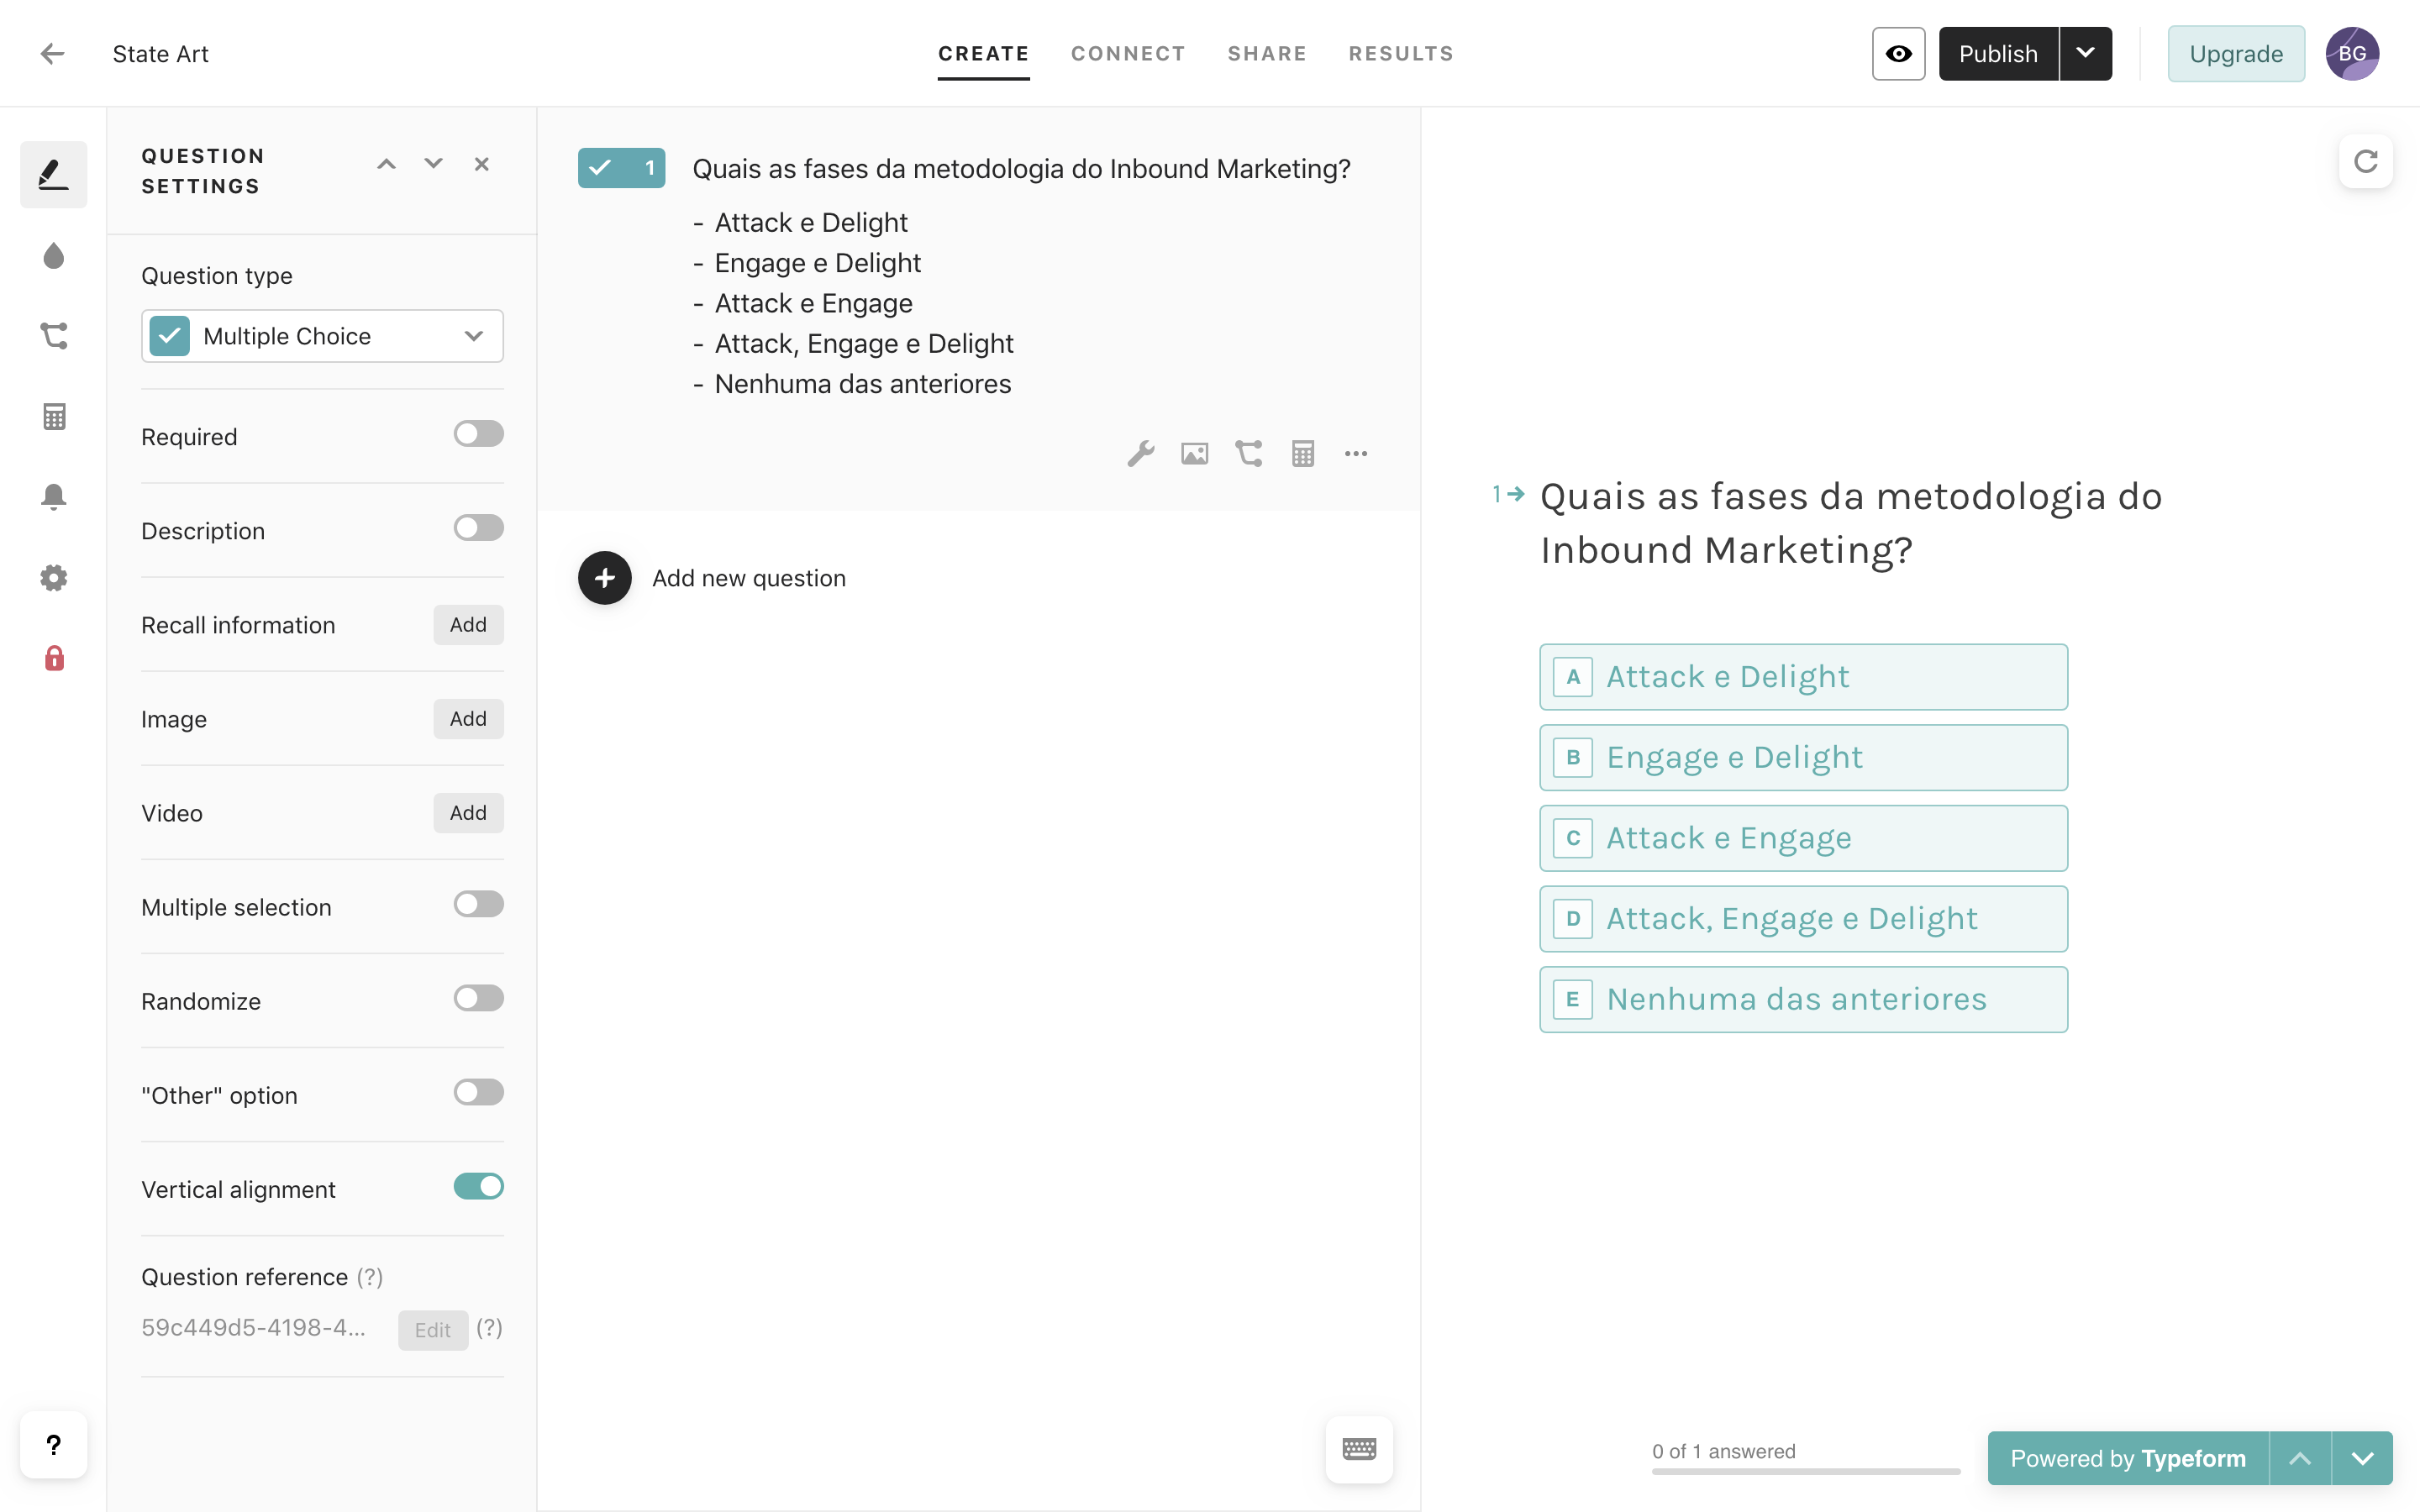
\includegraphics[width=1\textwidth]{img/tf/tf-question-opcoes}
		\caption{Typeform - Opções da pergunta}
		\label{fig:tf-question-opcoes}
	\end{center}
\end{figure}

\begin{figure}[ht!]
	\begin{center}
		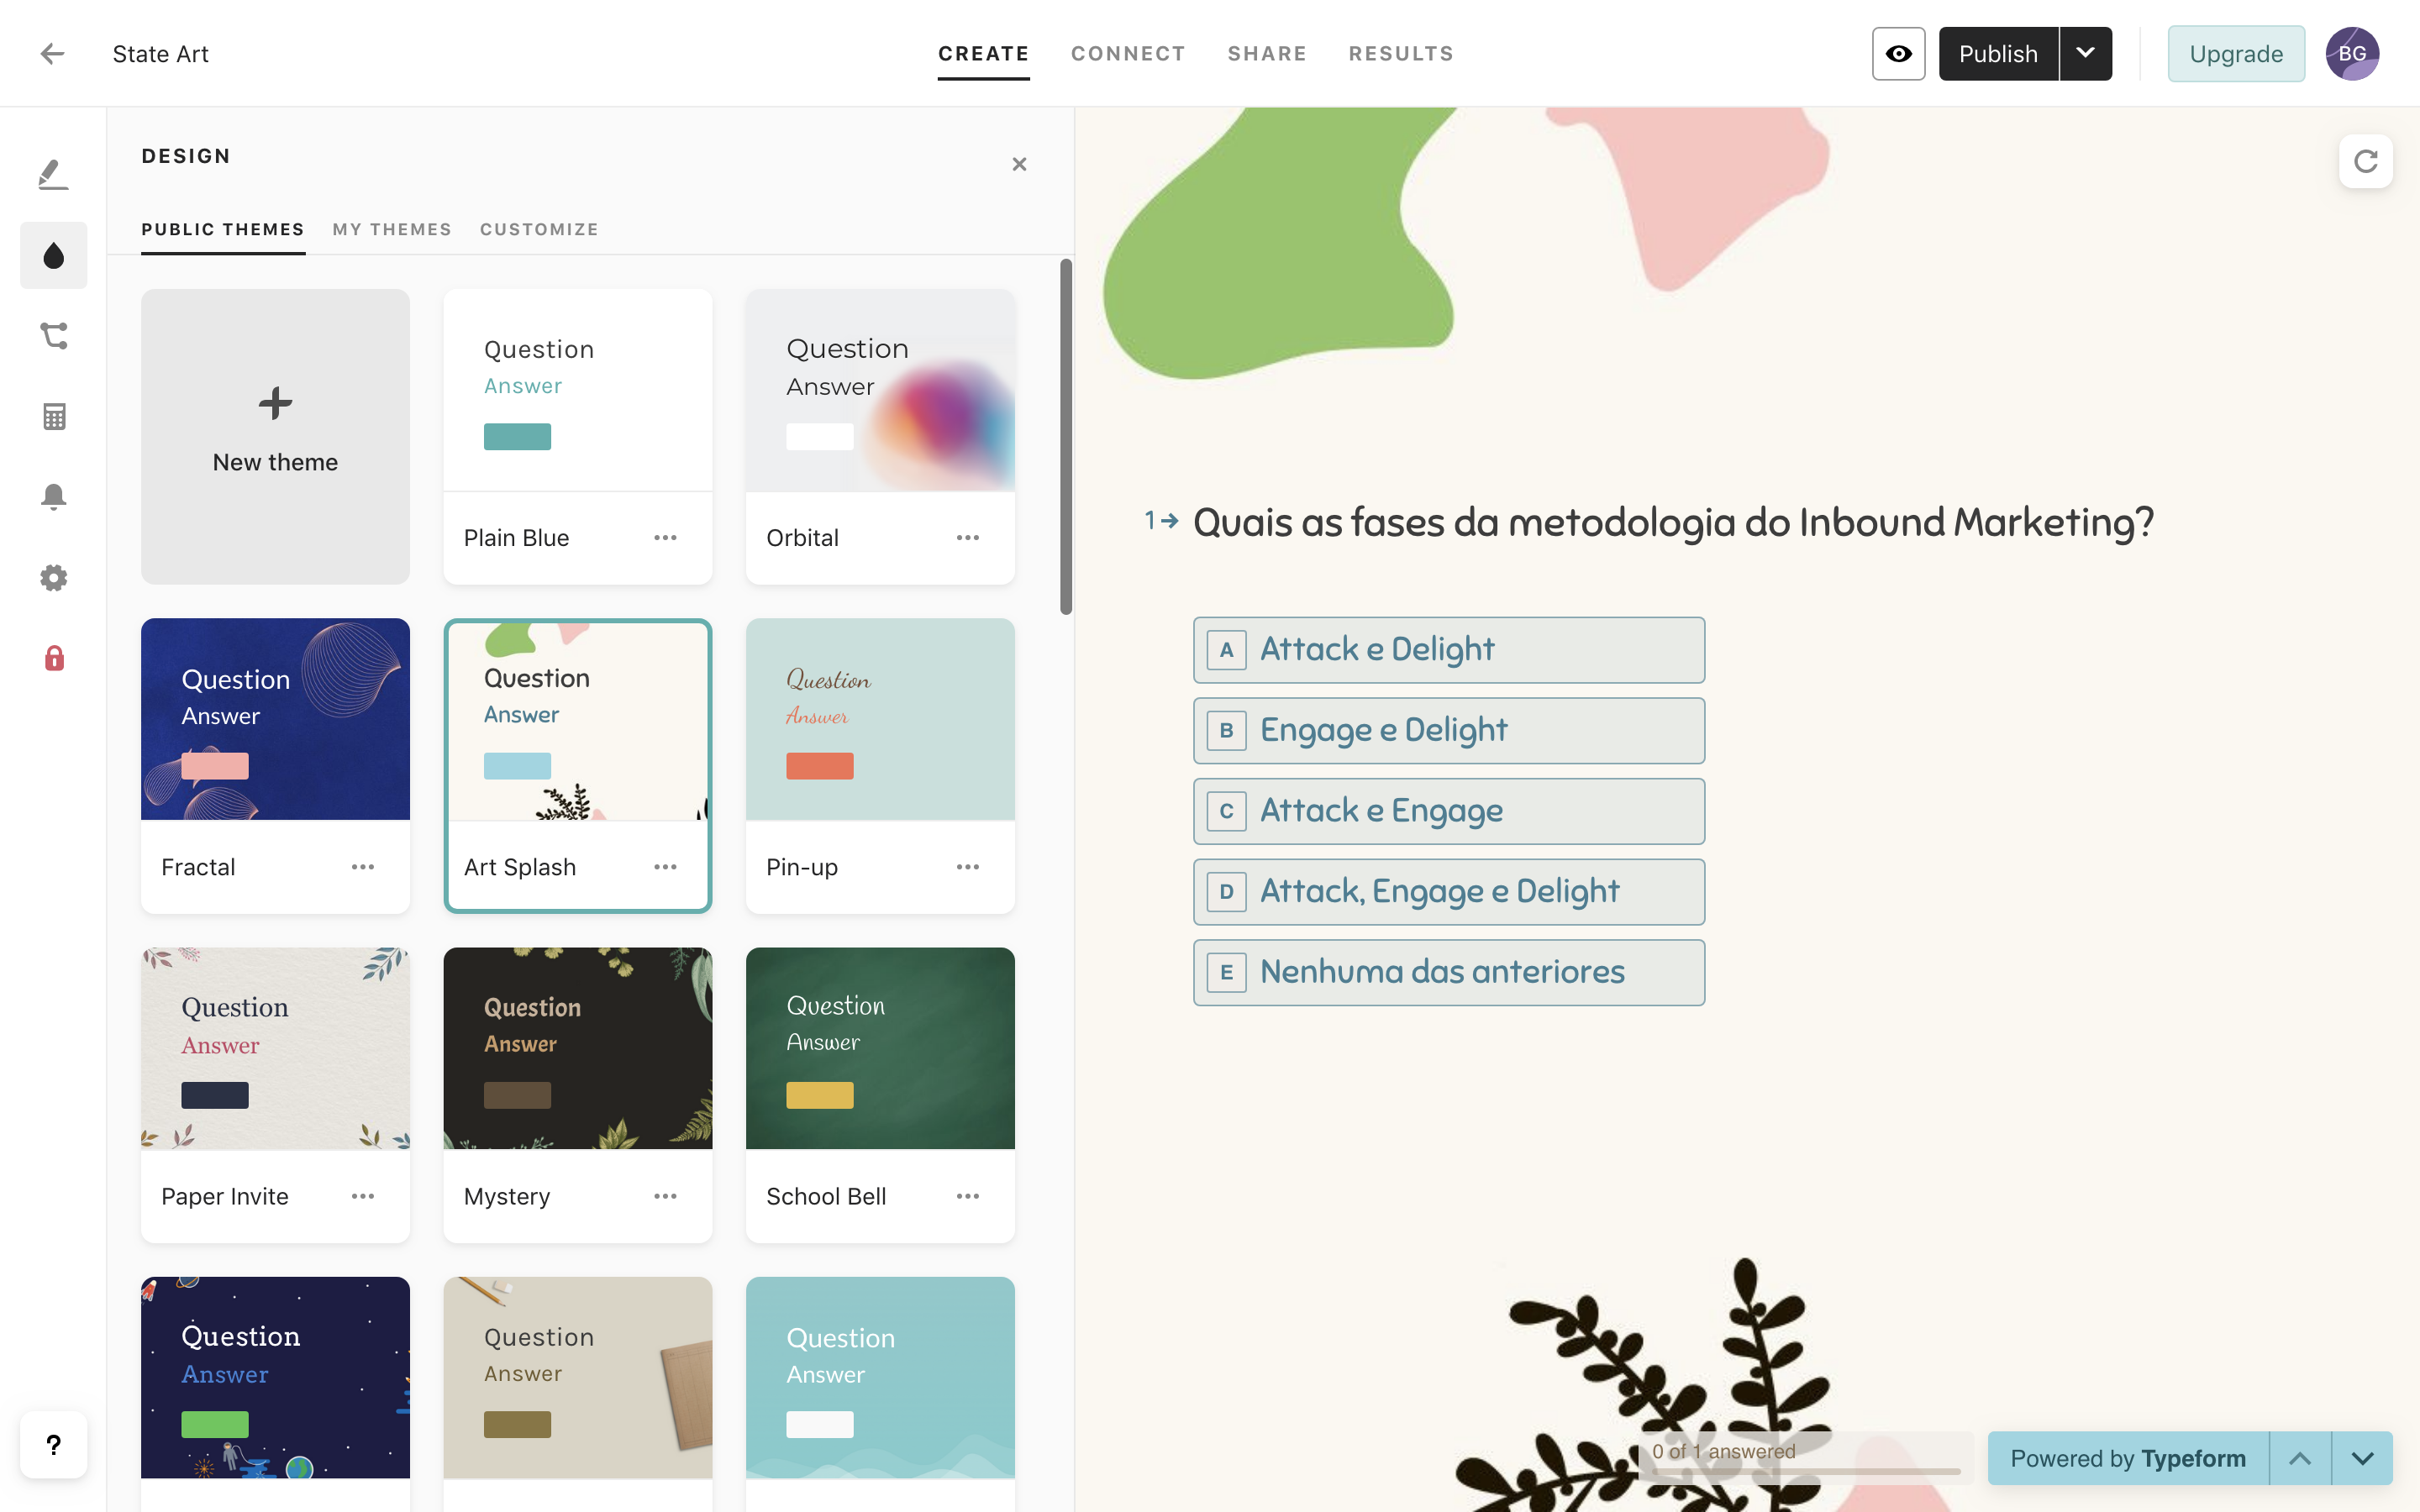
\includegraphics[width=1\textwidth]{img/tf/tf-question-custom}
		\caption{Typeform - Design da pergunta}
		\label{fig:tf-question-custom}
	\end{center}
\end{figure}
 
 A plataforma permite ainda os utilizadores adicionarem lógicas aos seus formulário, como exemplificado na Figura \ref{fig:tf-question-logica} , em que caso a resposta à pergunta 4 seja a especificada, o caminho a tomar será diferente. 
 

 
 \begin{figure}[ht!]
 	\begin{center}
 		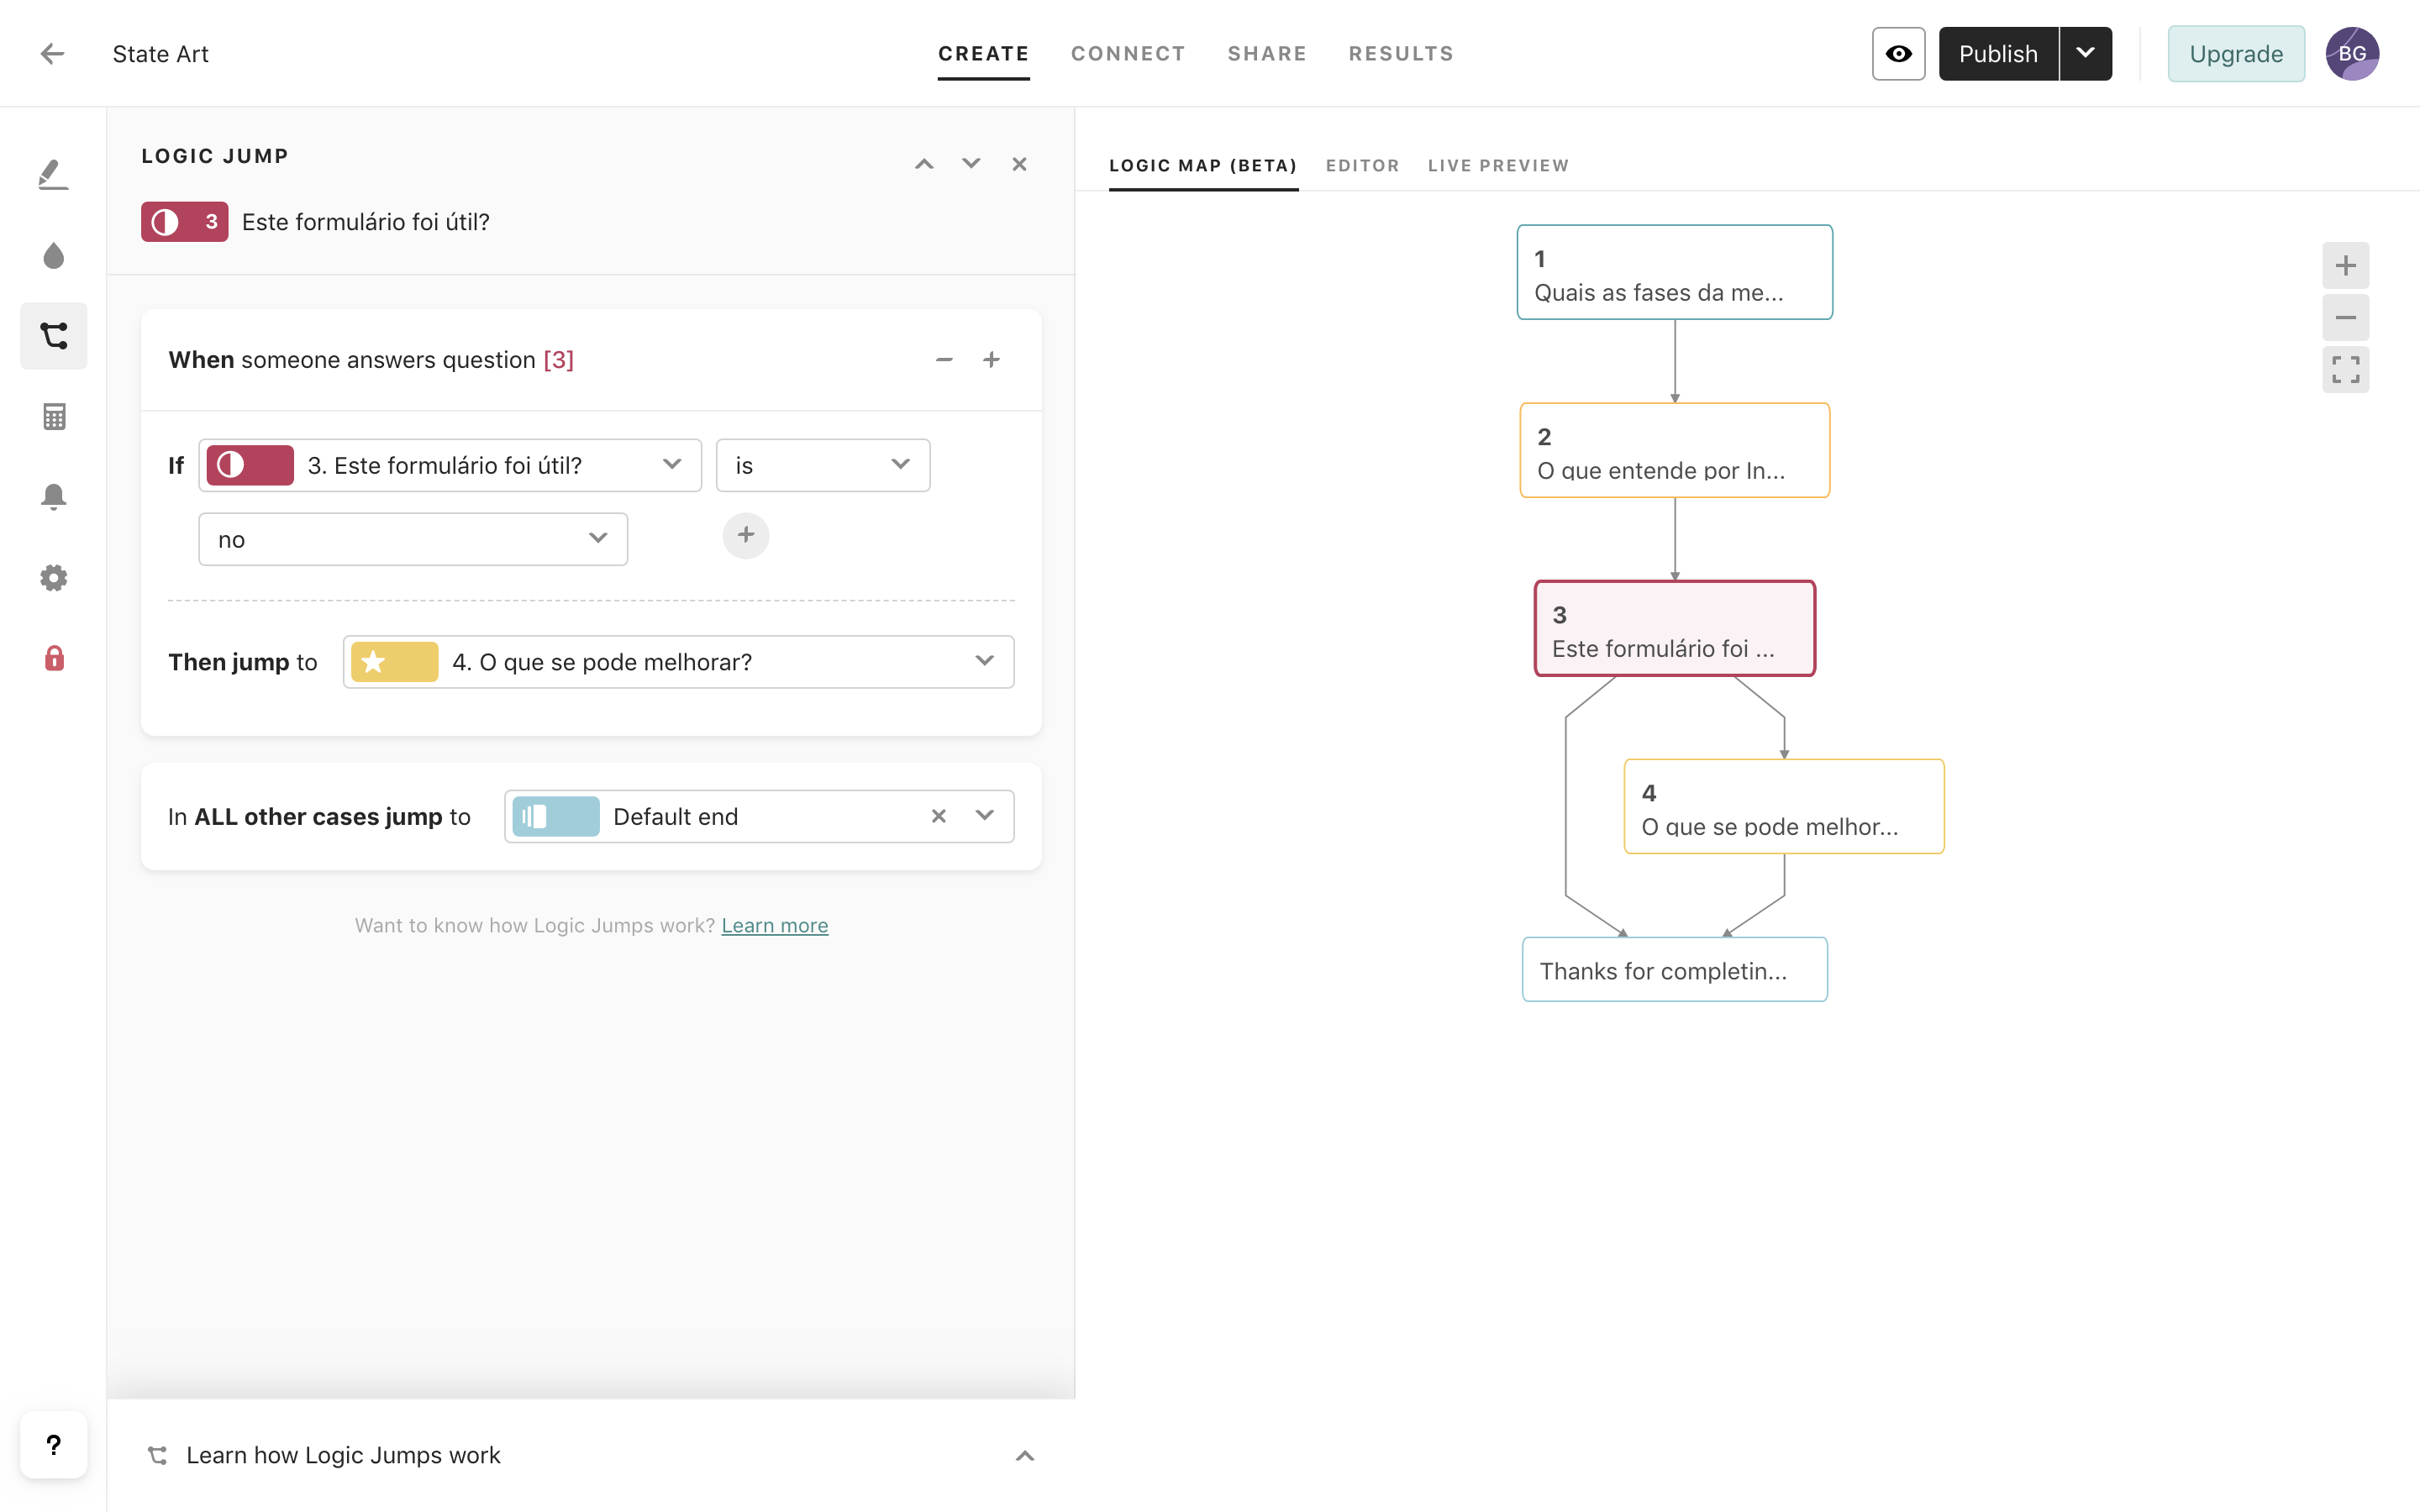
\includegraphics[width=1\textwidth]{img/tf/tf-question-logica}
 		\caption{Typeform - Lógica do formulário}
 		\label{fig:tf-question-logica}
 	\end{center}
 \end{figure}

\newpage

 A funcionalidade de visualizar o formulário está disponivel no canto superior direito, no lado esquerdo do botão de publicar, que permite o autor verificar se tudo está feito conforme planeado e assim poder publicar e partilhar.
 
 O Typeform permite também a integração de serviços externos com o formulário, como podemos ver na Figura \ref{fig:tf-question-integration} , em que, por exemplo, utilizando o Google Sheets\cite{googlesheets}, os resultados são exportados directamente para uma \textit{google sheet}


\begin{figure}[ht!]
	\begin{center}
		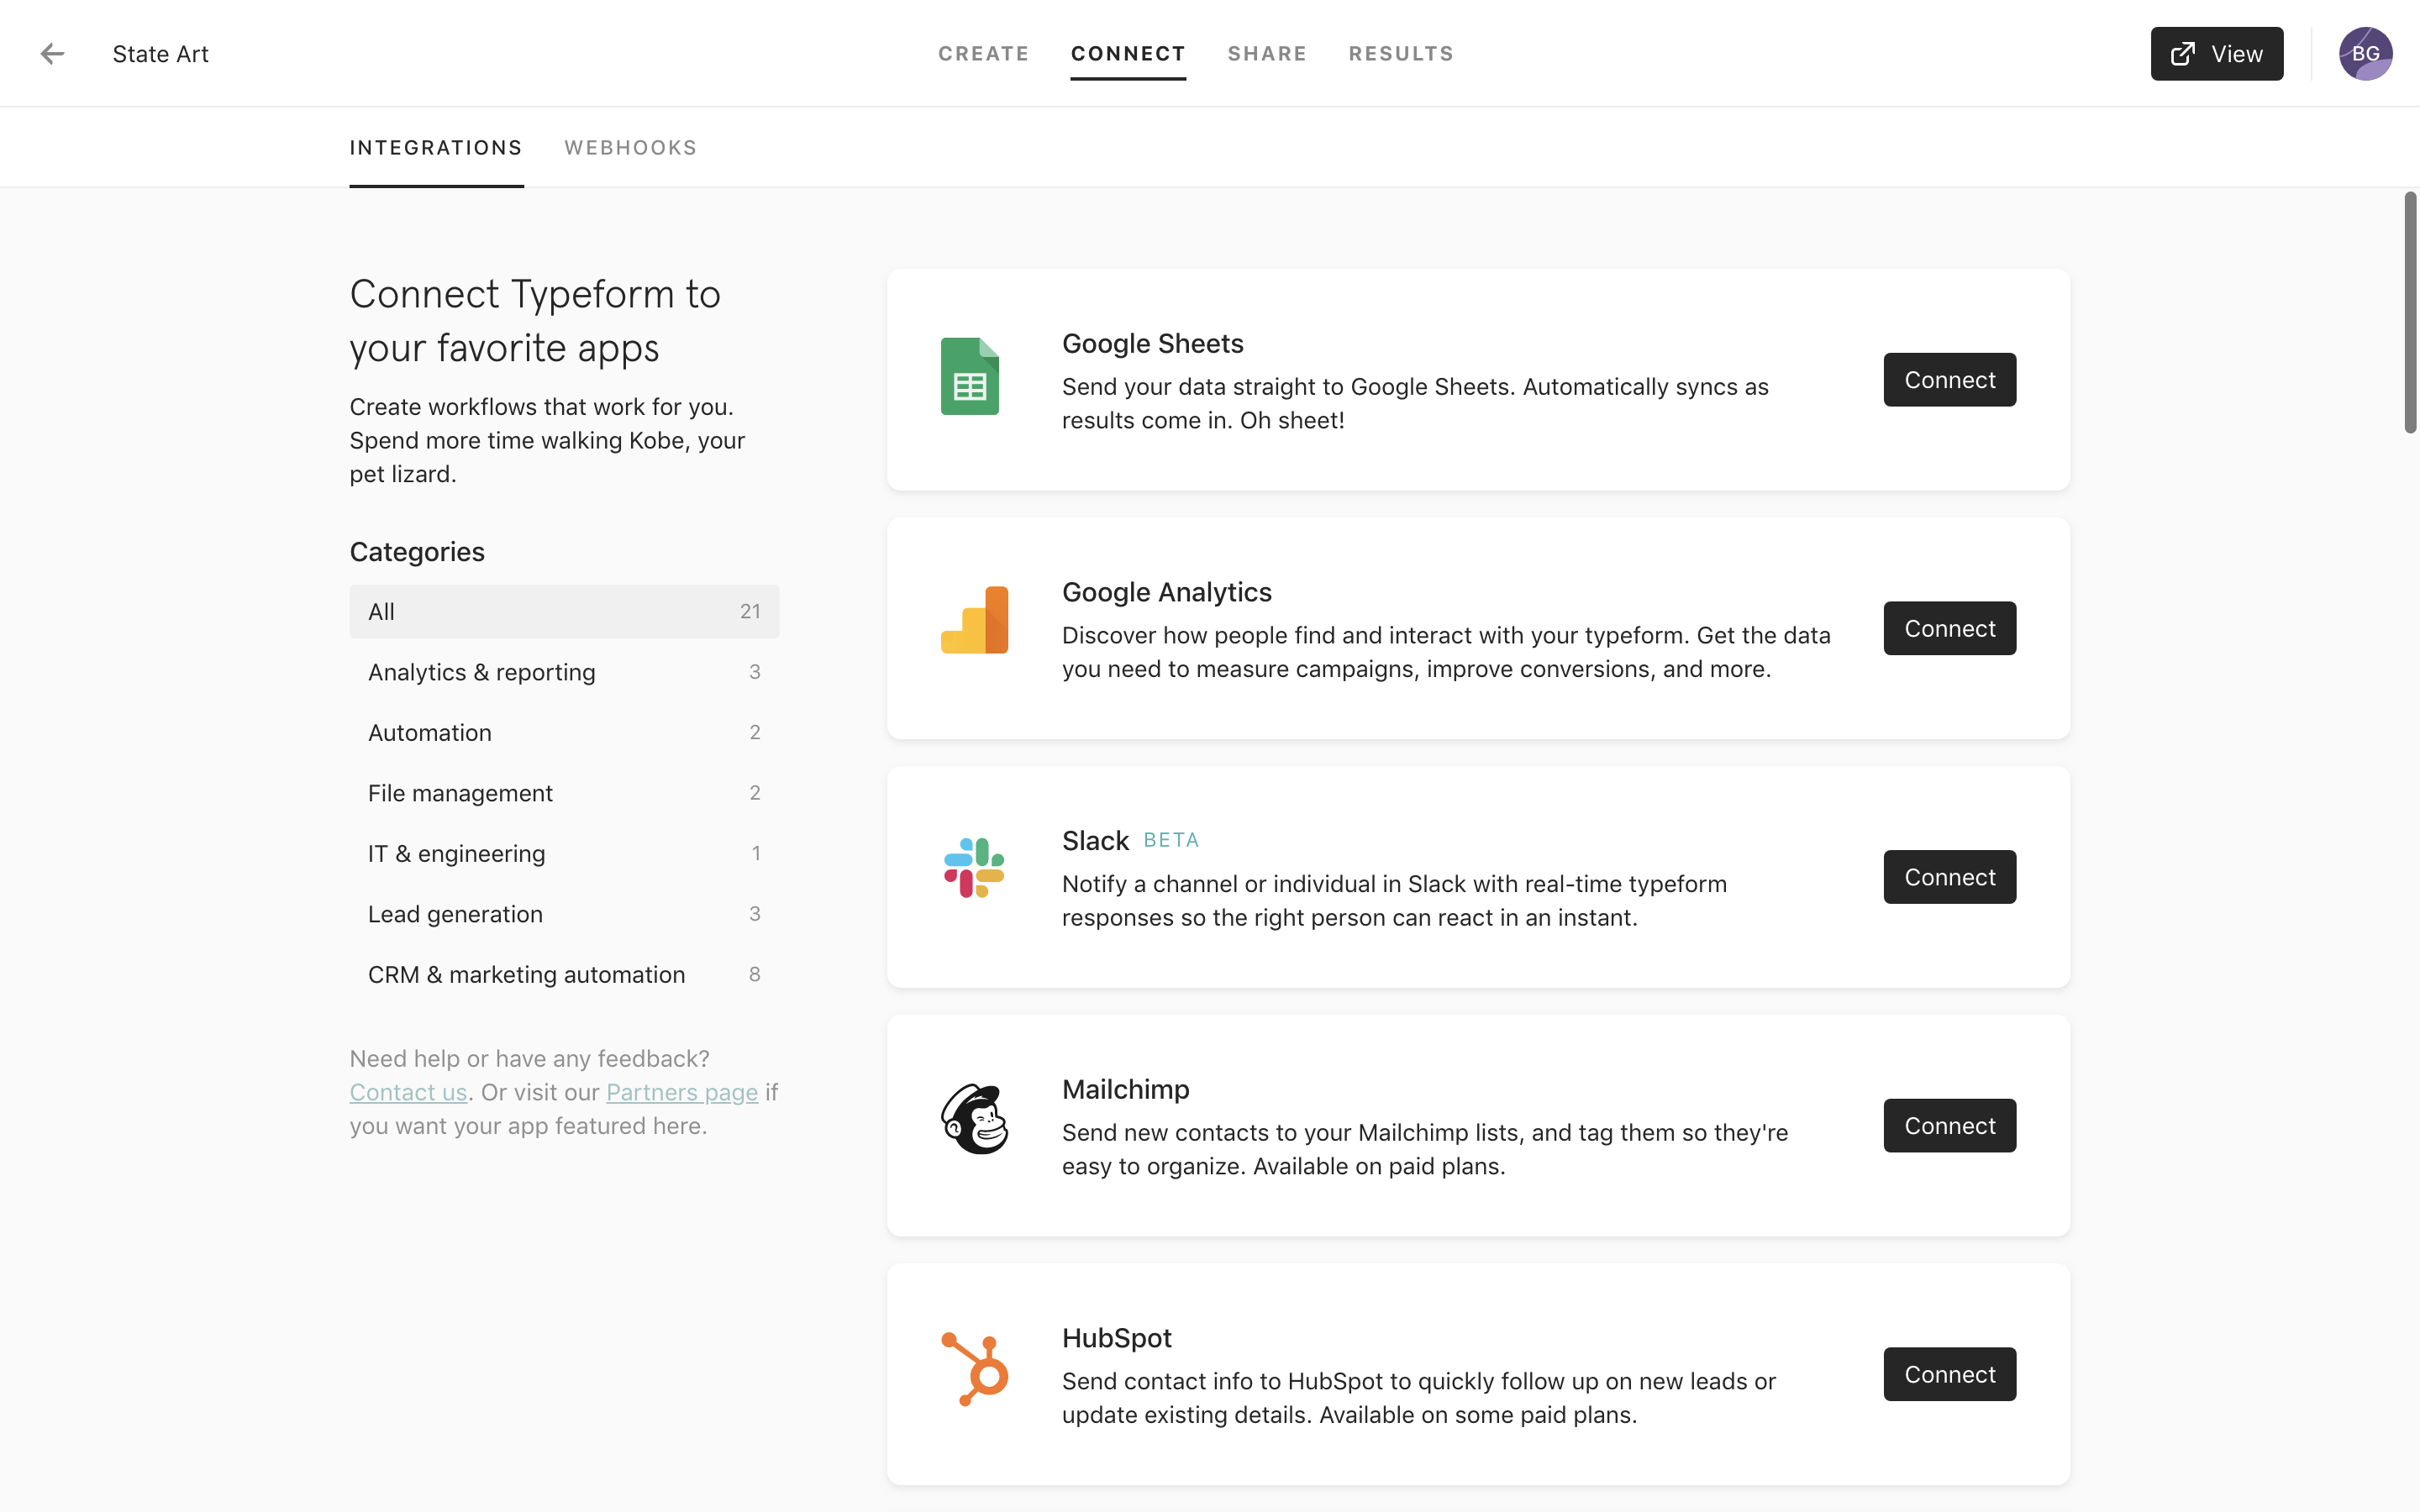
\includegraphics[width=1\textwidth]{img/tf/tf-question-integration}
		\caption{Typeform - Integração com sistemas externos}
		\label{fig:tf-question-integration}
	\end{center}
\end{figure}

Representado na Figura \ref{fig:tf-question-results} , temos a secção de analise de dados da plataforma onde podemos ver uma sumarização dos dados recebidos ou  analisar todas as respostas uma a uma. É também possível gerar um reportório dos dados recebidos e partilhar com alguém em qualquer fase, por exemplo, de uma campanha, uma vez que o mesmo é actualizado automaticamente com as novas respostas recebidas. 

O Typeform não fornece quaisquer filtros para segmentar os dados, contudo, fora as respostas em si, exibe algumas estatísticas/métricas relacionadas com os dispositivos que foram utilizados para responder aos formulários.


\newpage
\begin{figure}[ht!]
	\begin{center}
		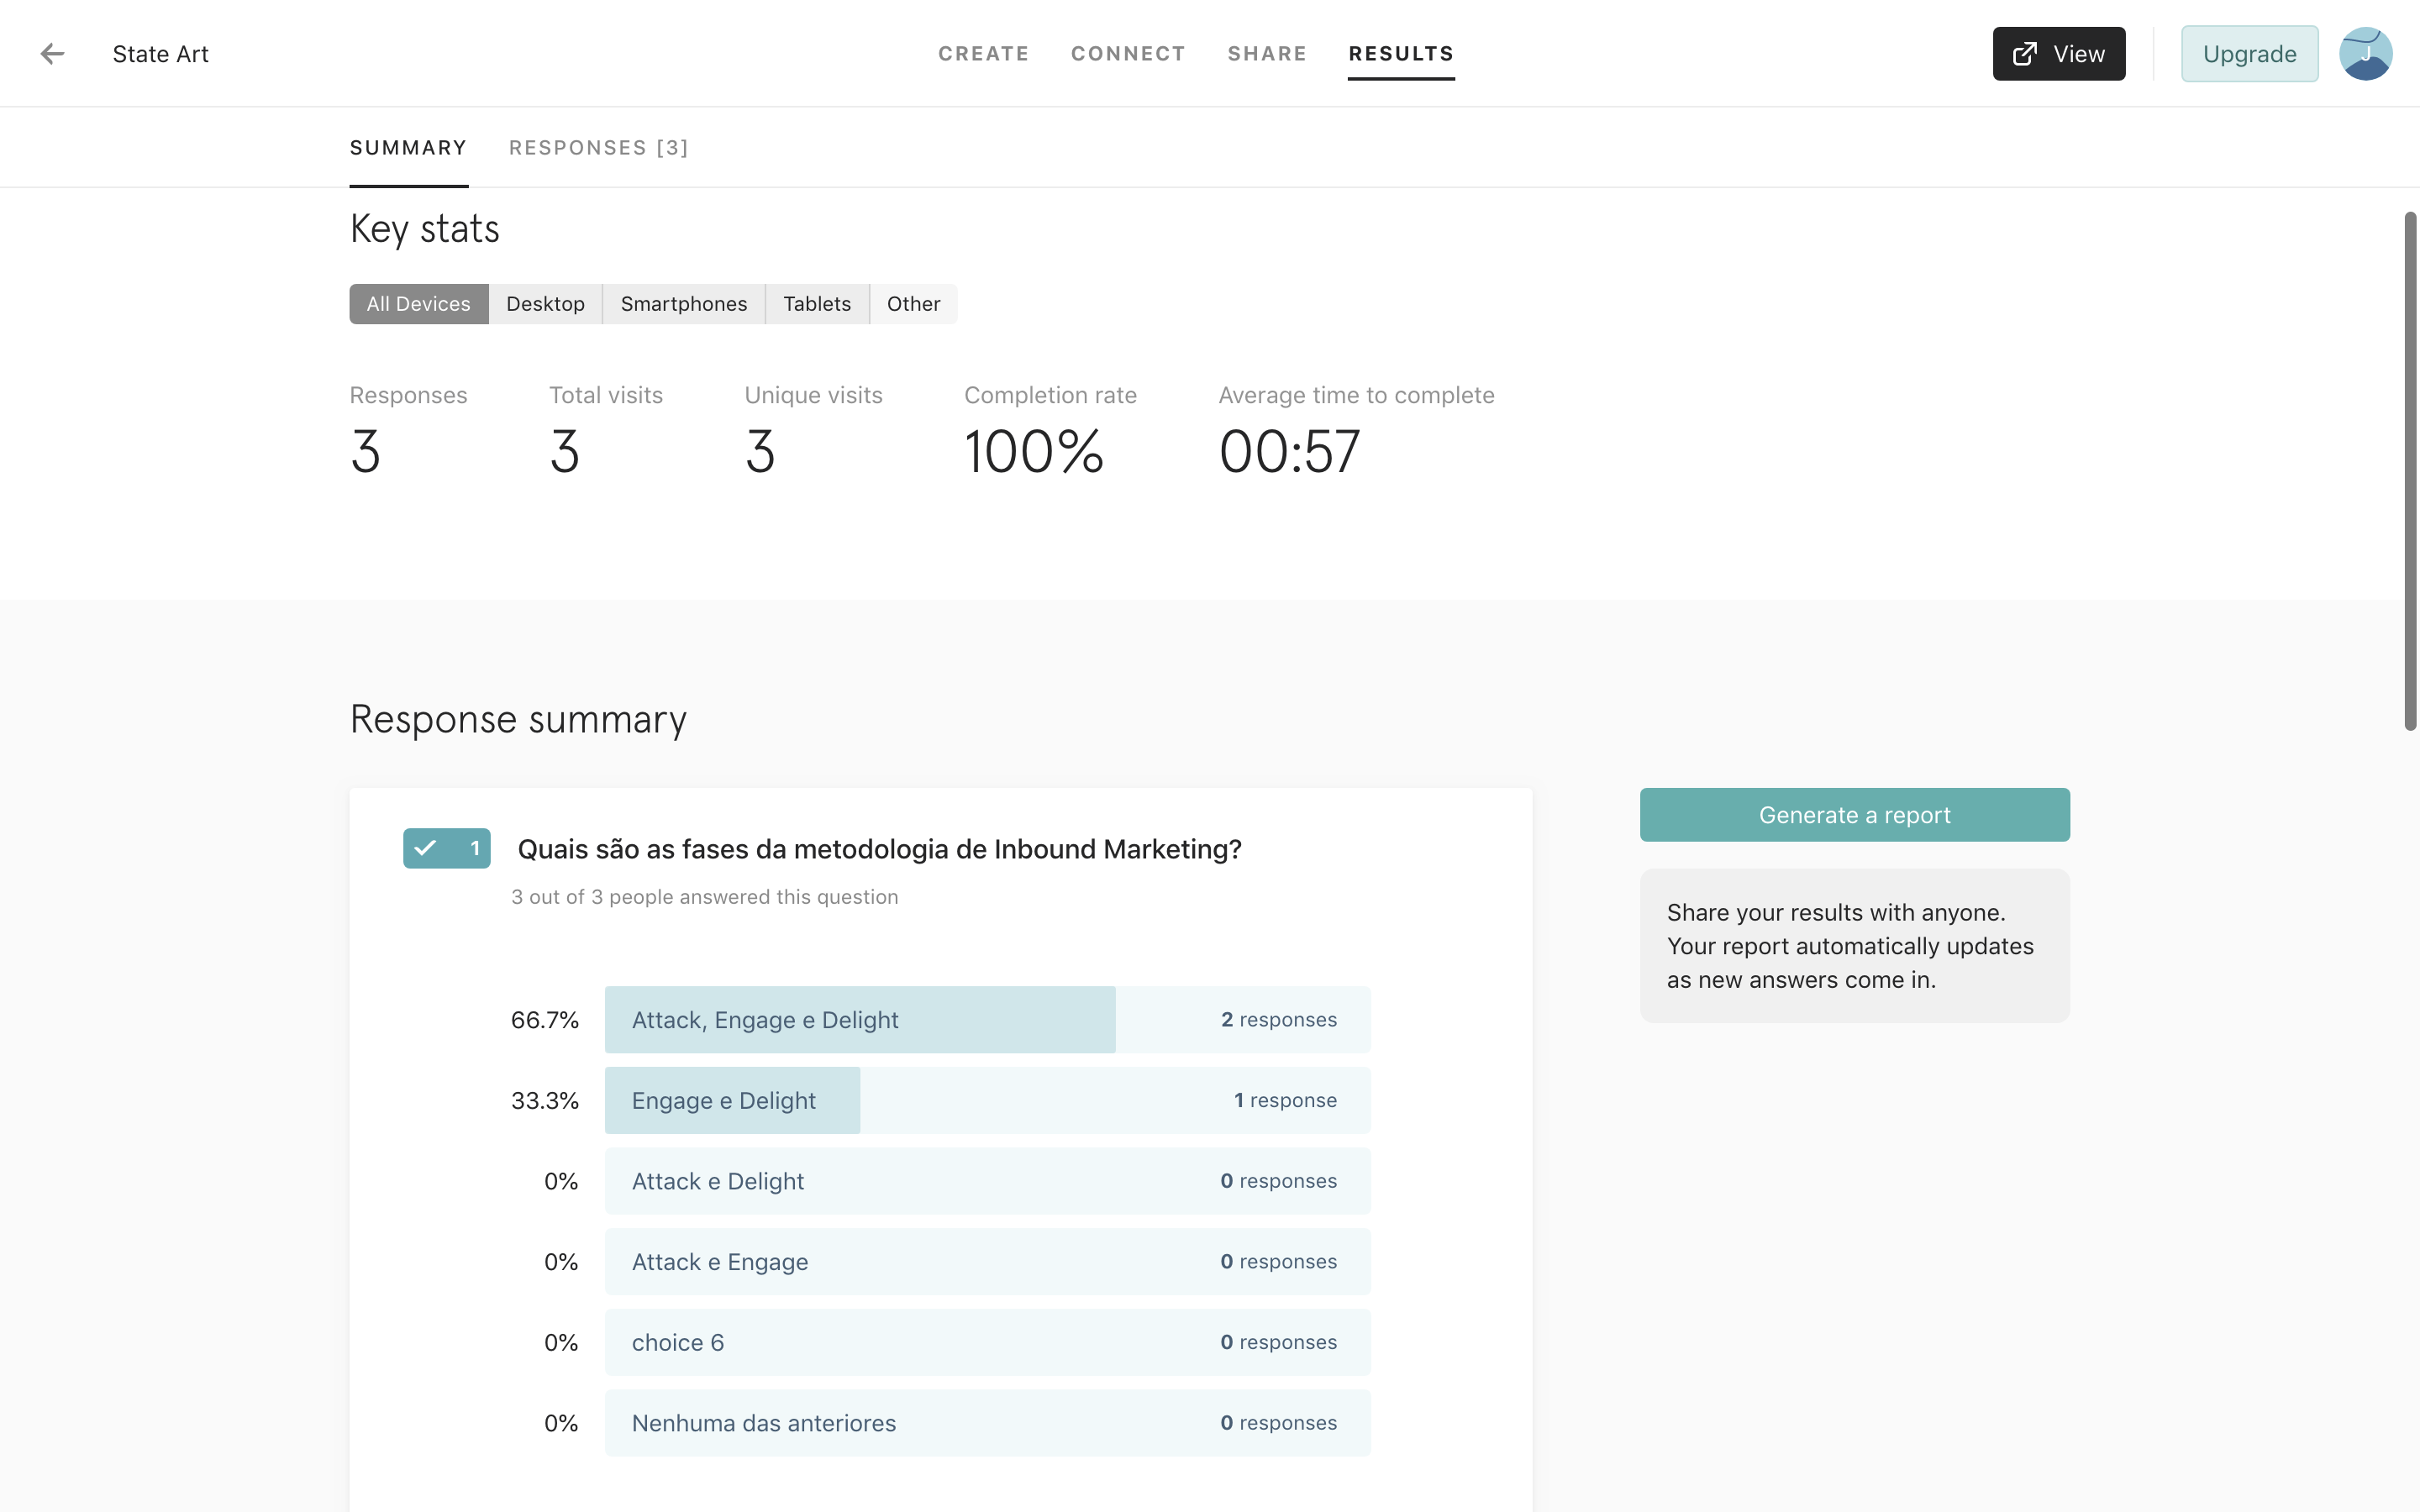
\includegraphics[width=1\textwidth]{img/tf/tf-question-results}
		\caption{Typeform - Analise de resultados}
		\label{fig:tf-question-results}
	\end{center}
\end{figure}



\section{Google Form}
\label{googleform}

O Google Form é uma aplicação de adminstração de inquéritos que está incluída no Google Drive office juntamente com o Google Docs\cite{gdocs}, Google Sheets e Google Slides\cite{gslides}. Esta ferramenta permite recolher informações do público alvo através de formulários e inquéritos personalizados e automaticamente exportar os dados para uma \textit{google sheet}.

Estam aplicação é totalmente gratuita, bastanto apenas criar uma conta Google\cite{gaccount} para poder aceder a todas as funcionalidades da ferramenta.

Representado na Figura \ref{fig:gf-dashboard}, está o painel de controlo da conta de um utilizador, onde o mesmo pode visualizar os formulários com que interagiu recentemente. Por cima dos formulários recentes temos o butão para criar um novo formulário juntamente com alguns \textit{templates}/recomendações de formulários.

\newpage

\begin{figure}[ht!]
	\begin{center}
		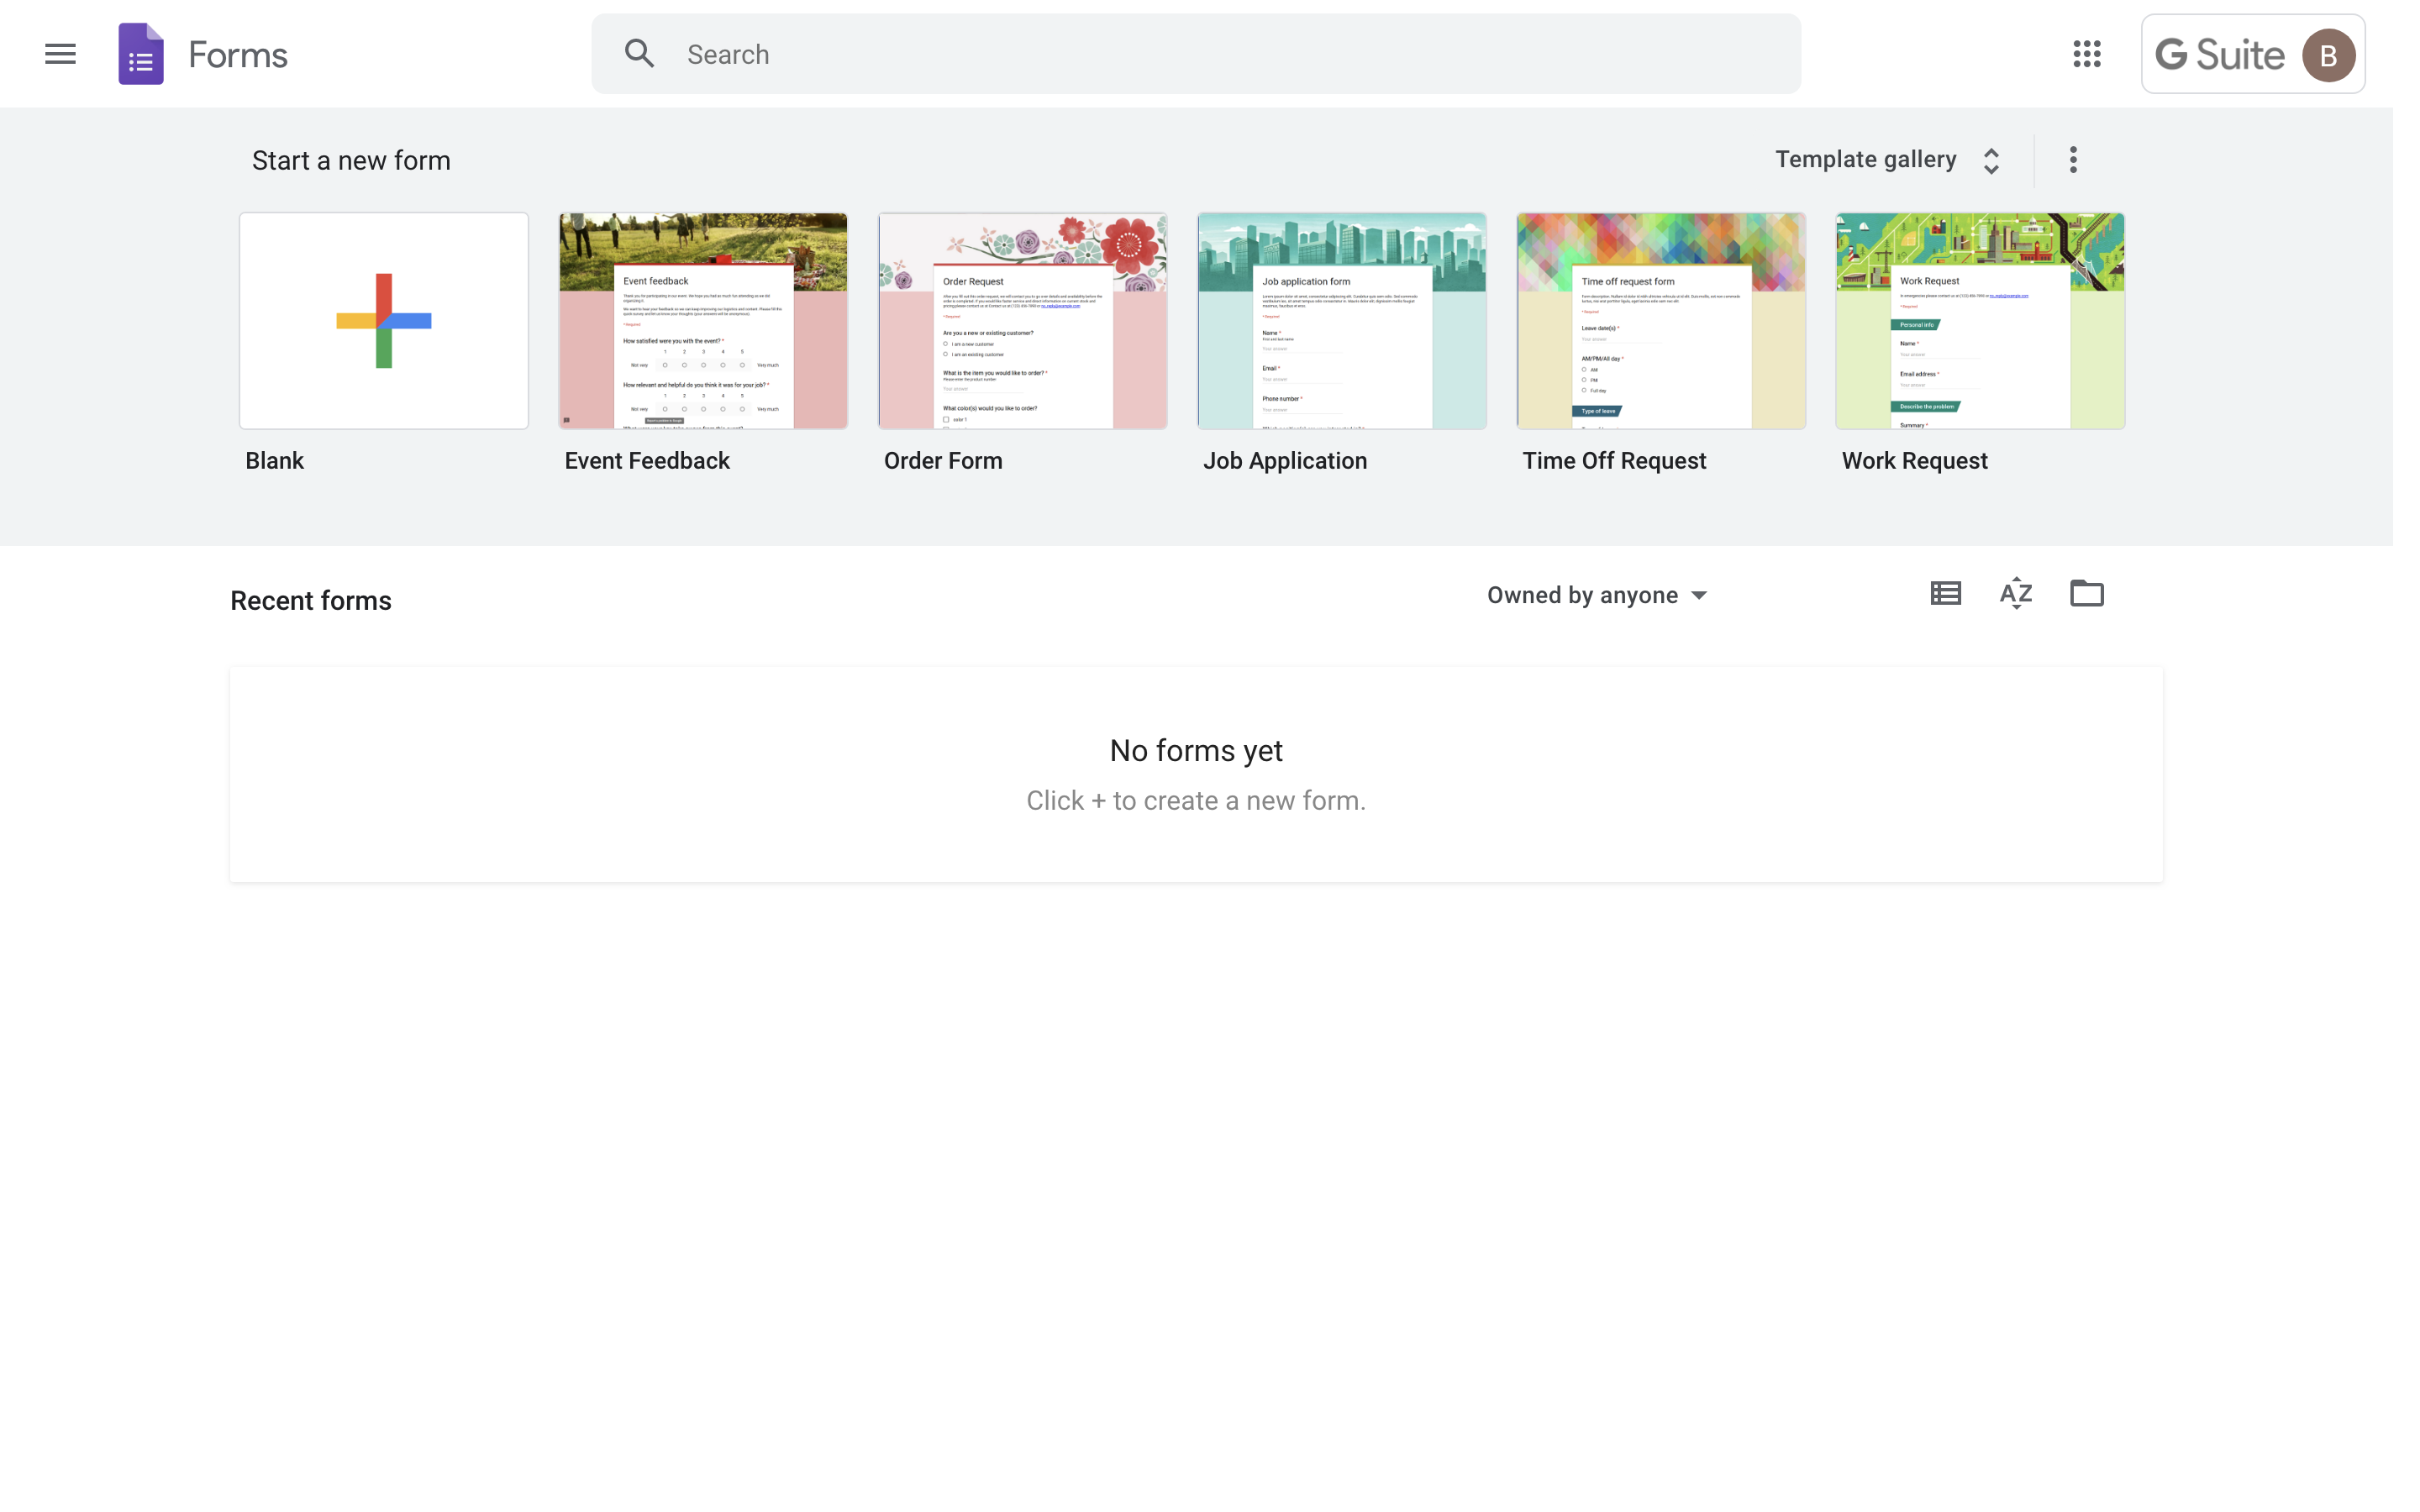
\includegraphics[width=1\textwidth]{img/gf/gf-dashboard}
		\caption{Google Form - Painel de Controlo}
		\label{fig:gf-dashboard}
	\end{center}
\end{figure}


\begin{figure}[ht!]
	\begin{center}
		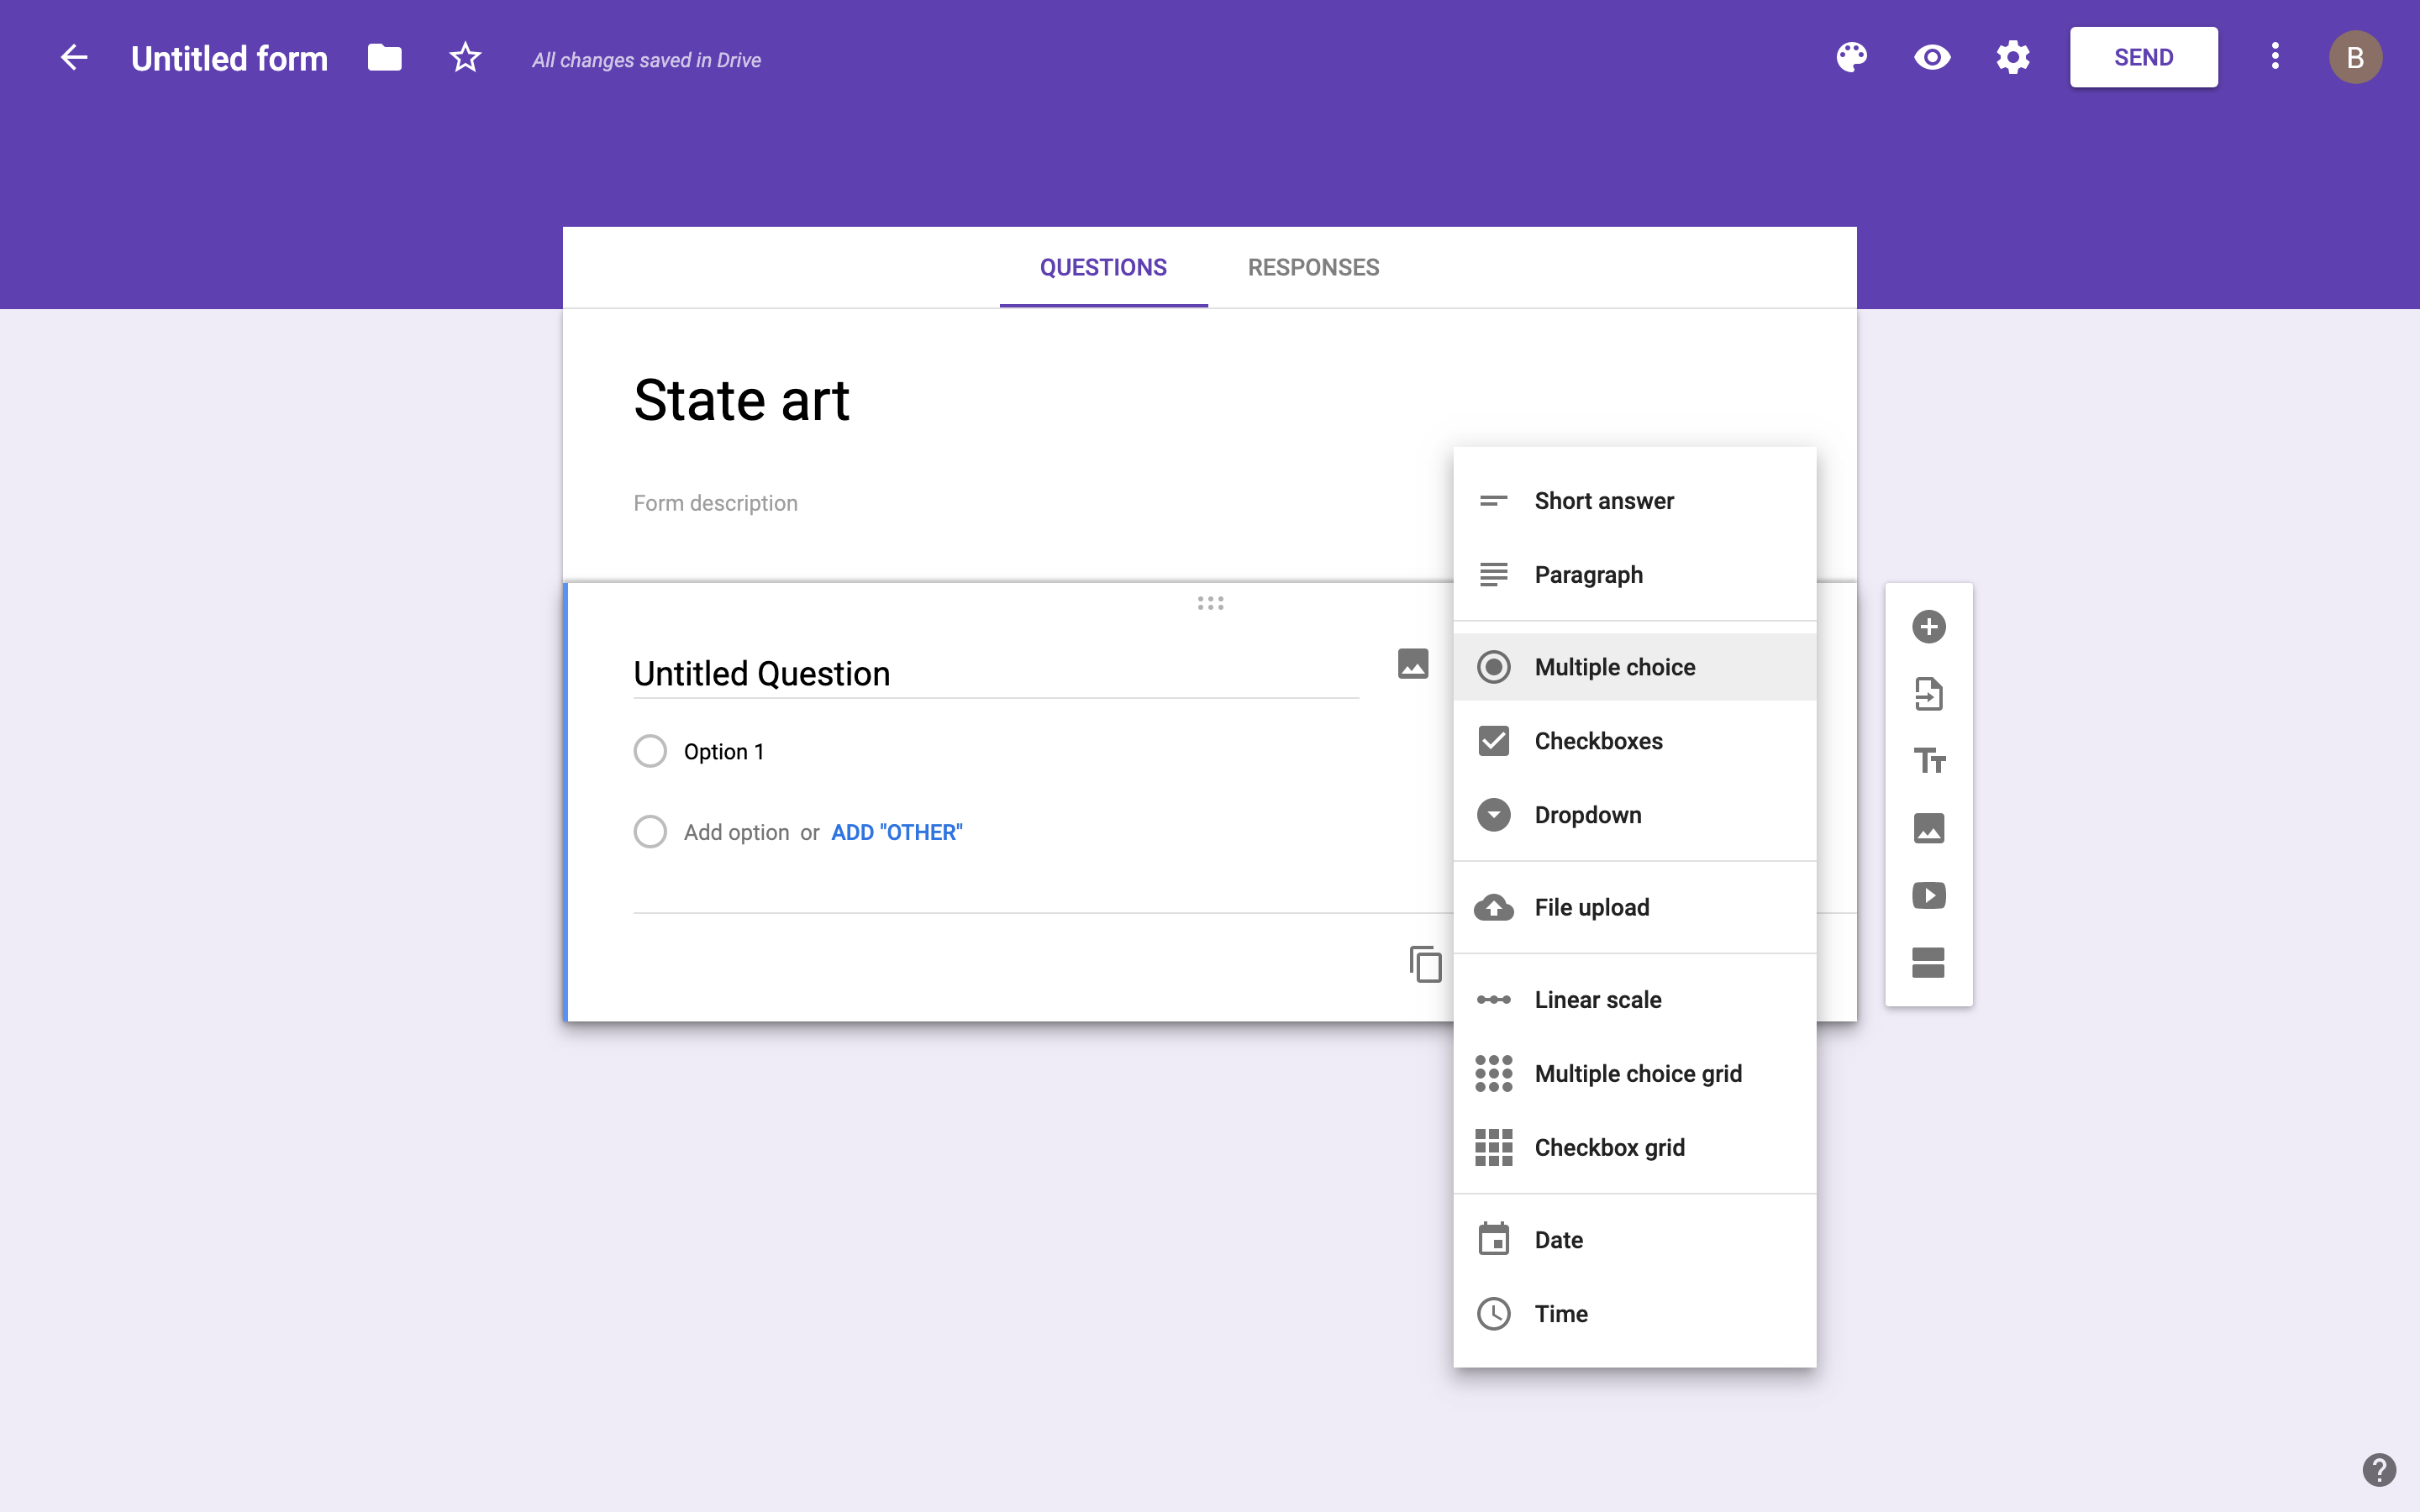
\includegraphics[width=1\textwidth]{img/gf/gf-form-q-type}
		\caption{Google Form - Tipos de perguntas}
		\label{fig:gf-form-q-type}
	\end{center}
\end{figure}

A Figura \ref{fig:gf-form-q-type} demonstra a criação de um formulário do zero. Há vários tipo de perguntas que a aplicação permite adicionar ao formulário e, apesar de se estar a criar um formulário novo, o google form permite importar um ou mais formulários diferentes, ao qual o utilizador tem acesso (i. e. formulários que estão disponíveis na sua área de trabalho), selecionando apenas as perguntas que deseja importar. Como podemos ver nas Figuras \ref{fig:gf-form-import}, \ref{fig:gf-form-import-select} e \ref{fig:gf-form-imported} as perguntas importadas foram colocadas na posição escolhida, que neste caso foi no final do formulário.

\begin{figure}[h!]
	\begin{center}
		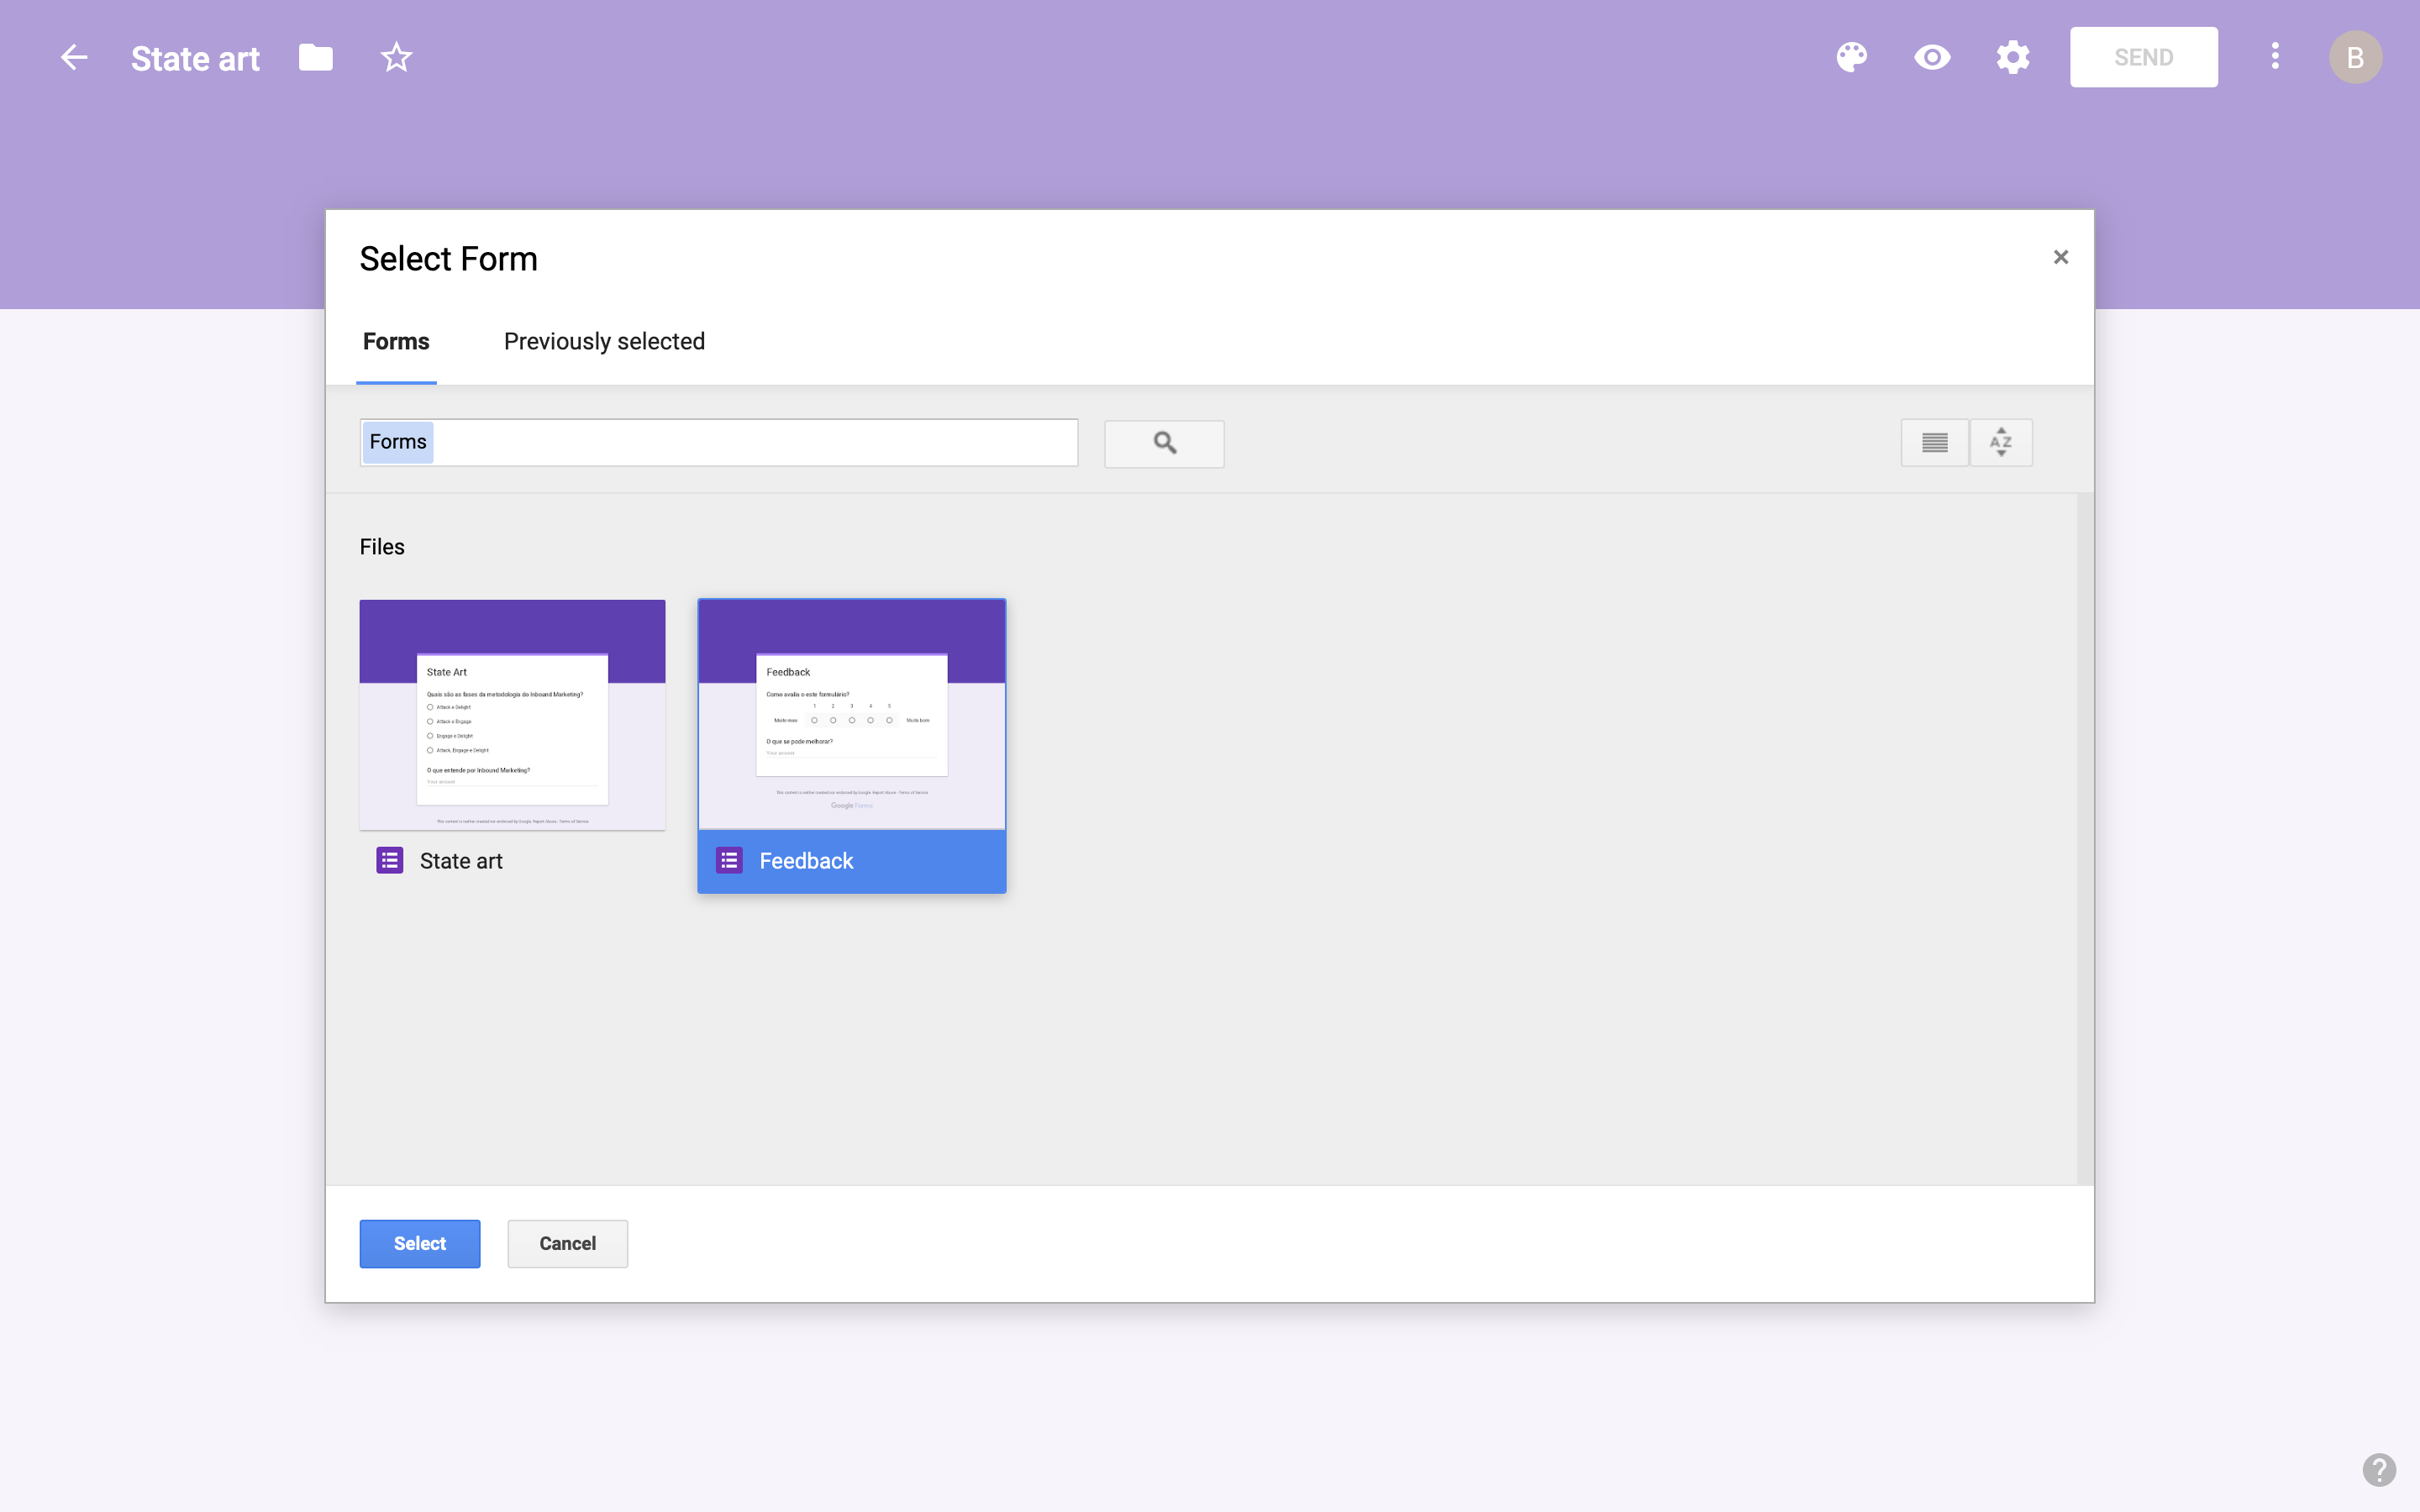
\includegraphics[width=1\textwidth]{img/gf/gf-form-import}
		\caption{Google Form - Importar formulário}
		\label{fig:gf-form-import}
	\end{center}
\end{figure}

\begin{figure}[h!]
	\begin{center}
		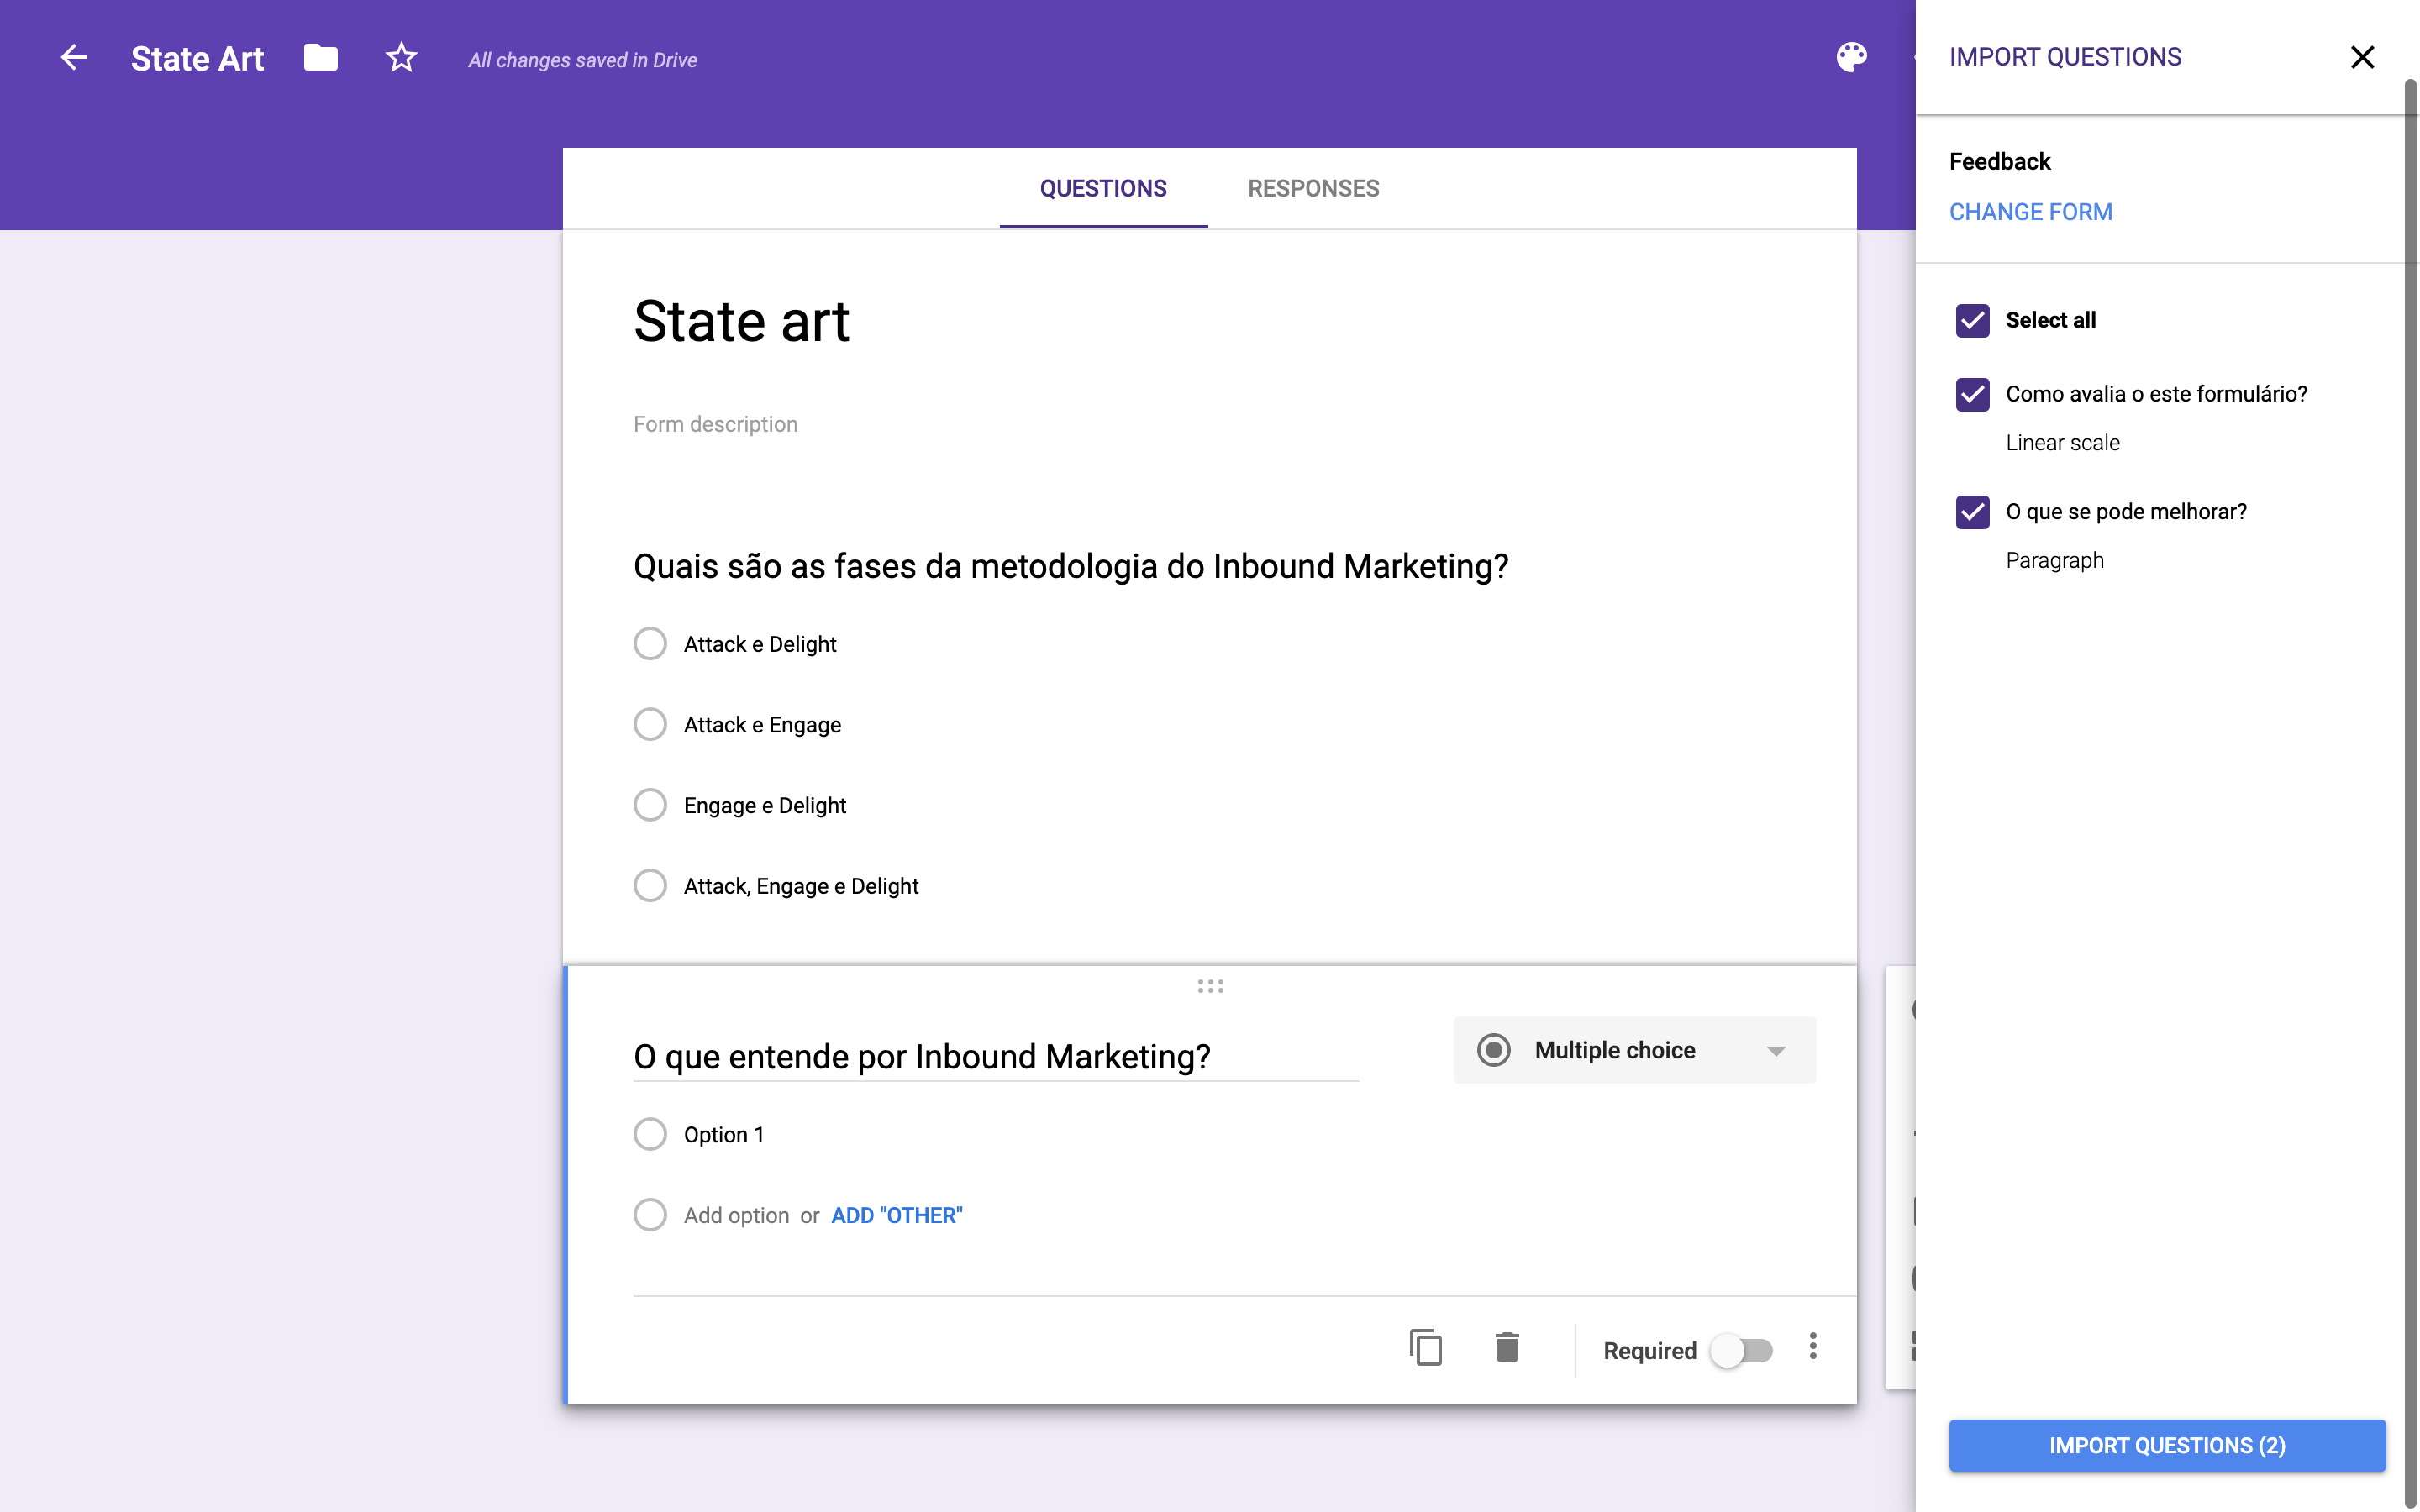
\includegraphics[width=1\textwidth]{img/gf/gf-form-import-select}
		\caption{Google Form - Selecionar perguntas a importar}
		\label{fig:gf-form-import-select}
	\end{center}
\end{figure}

\begin{figure}[h!]
	\begin{center}
		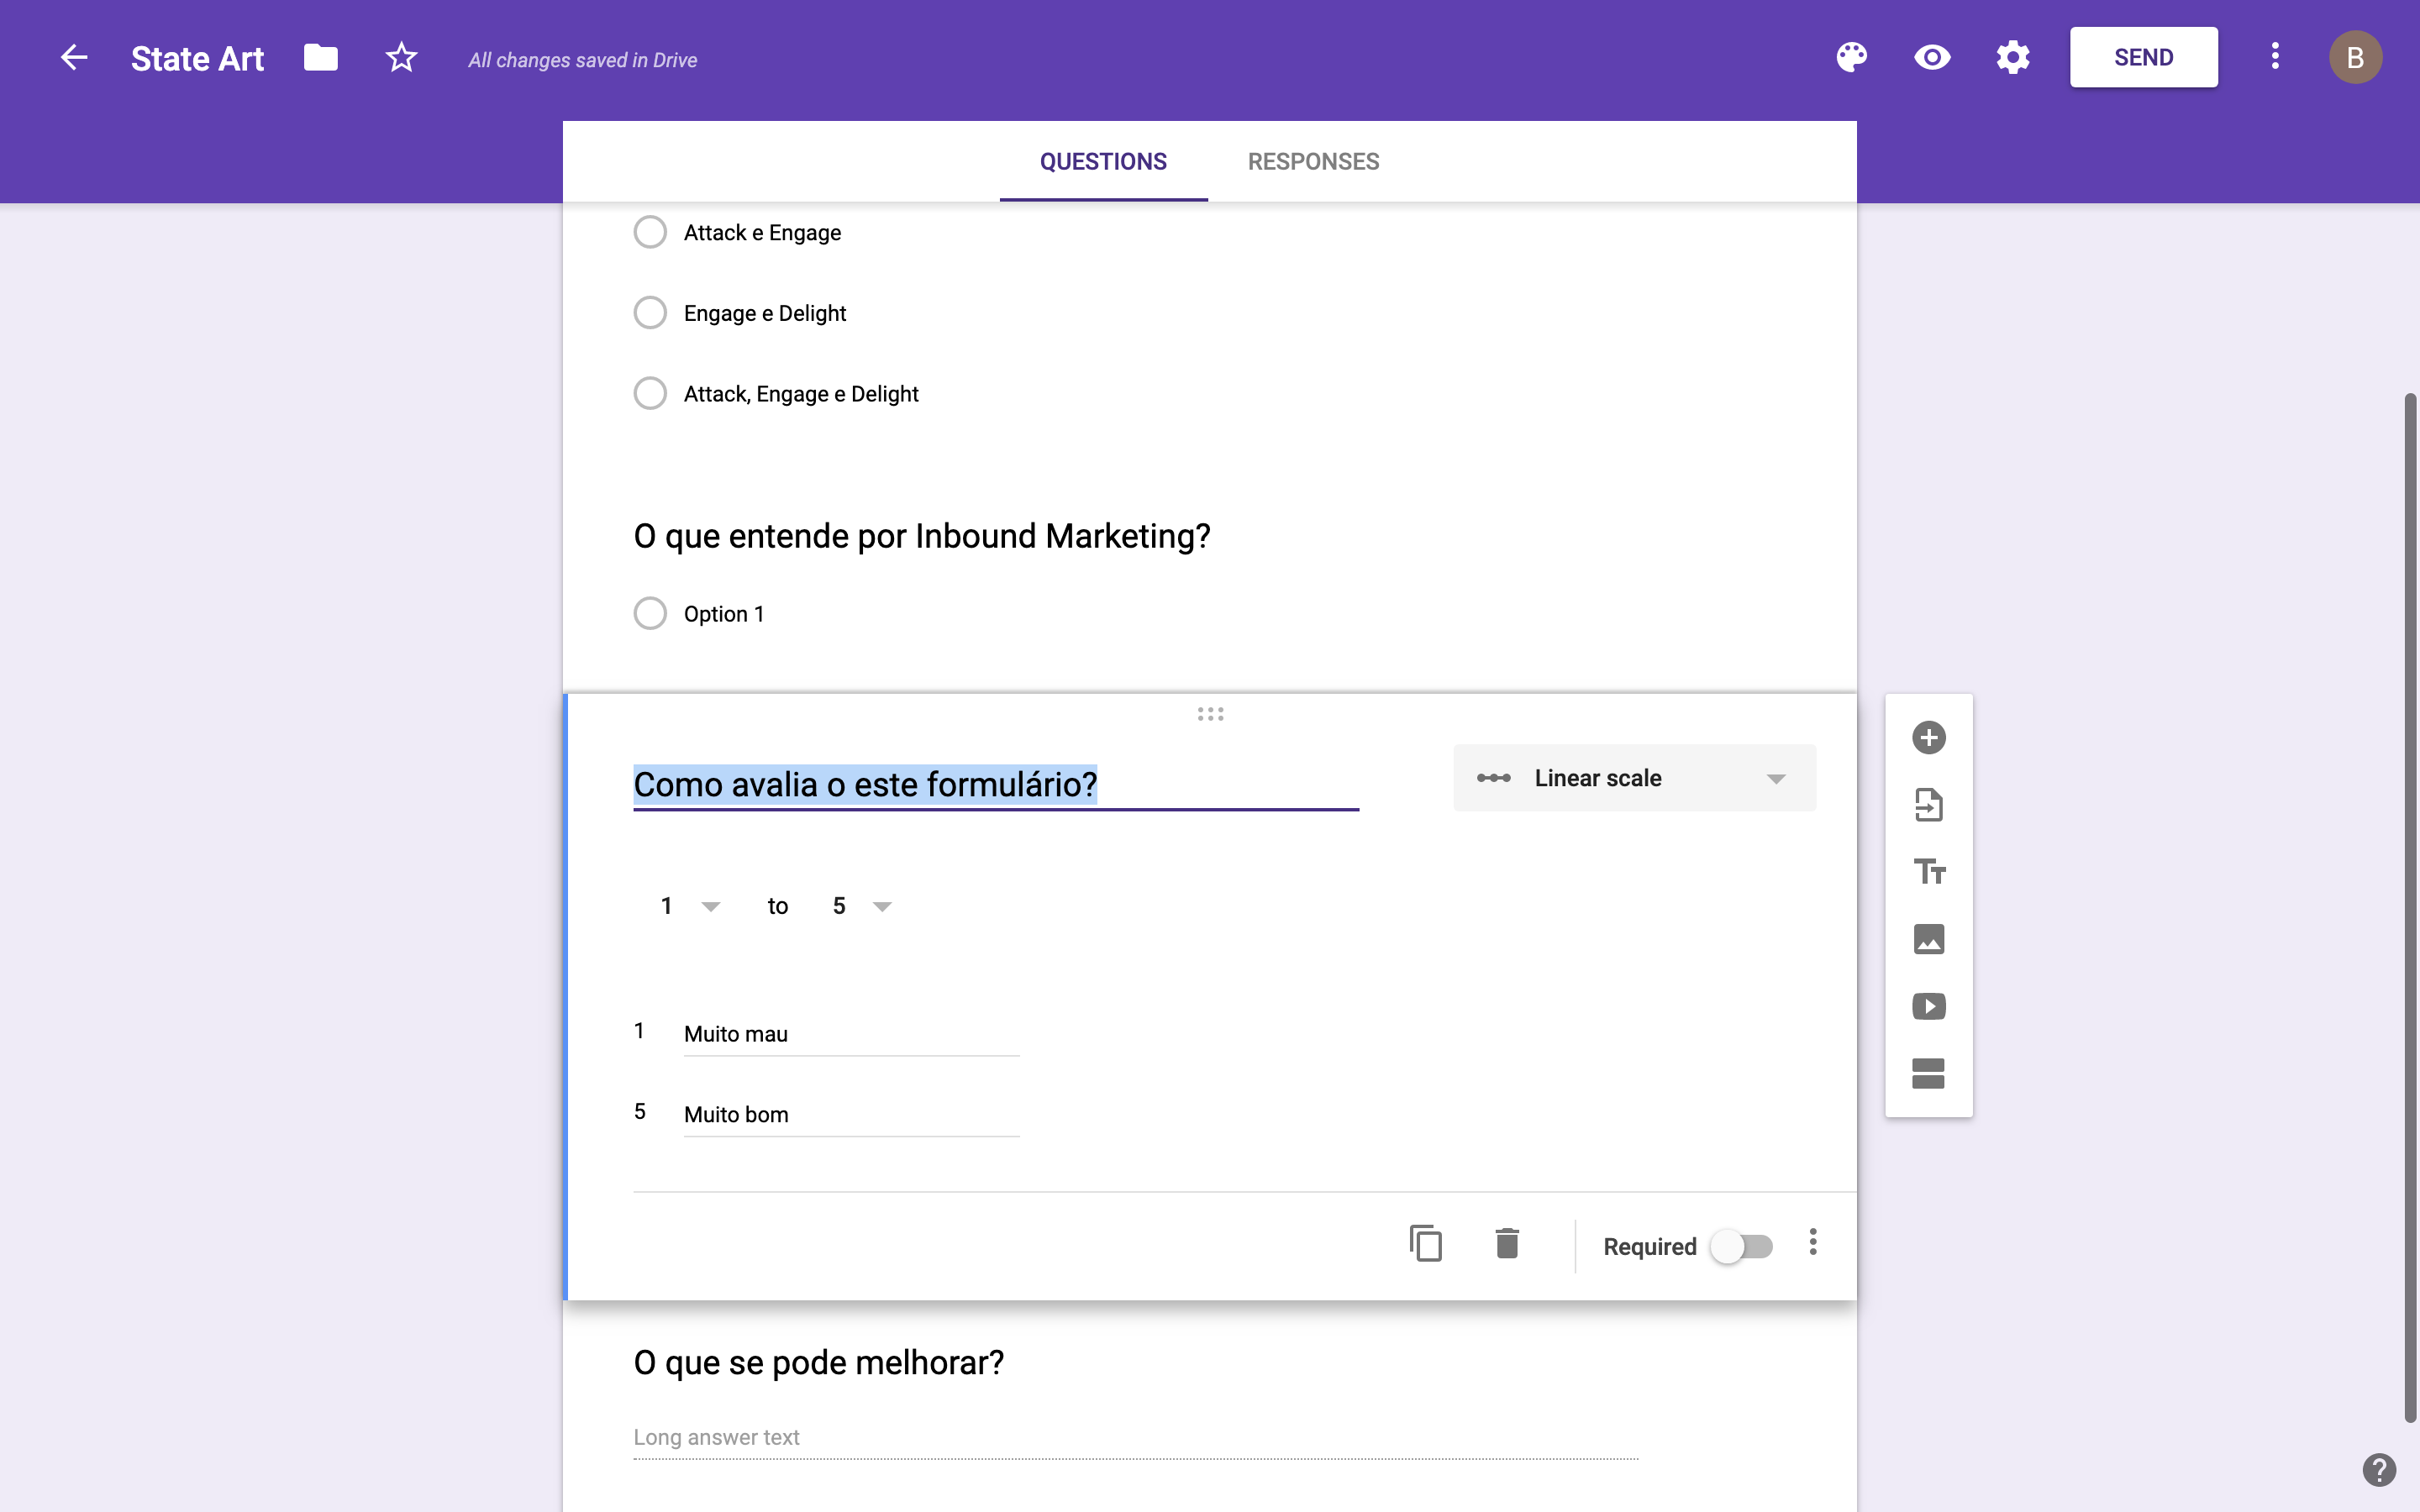
\includegraphics[width=1\textwidth]{img/gf/gf-form-imported}
		\caption{Google Form - Perguntas importadas}
		\label{fig:gf-form-imported}
	\end{center}
\end{figure}


\begin{figure}[h!]
	\begin{center}
		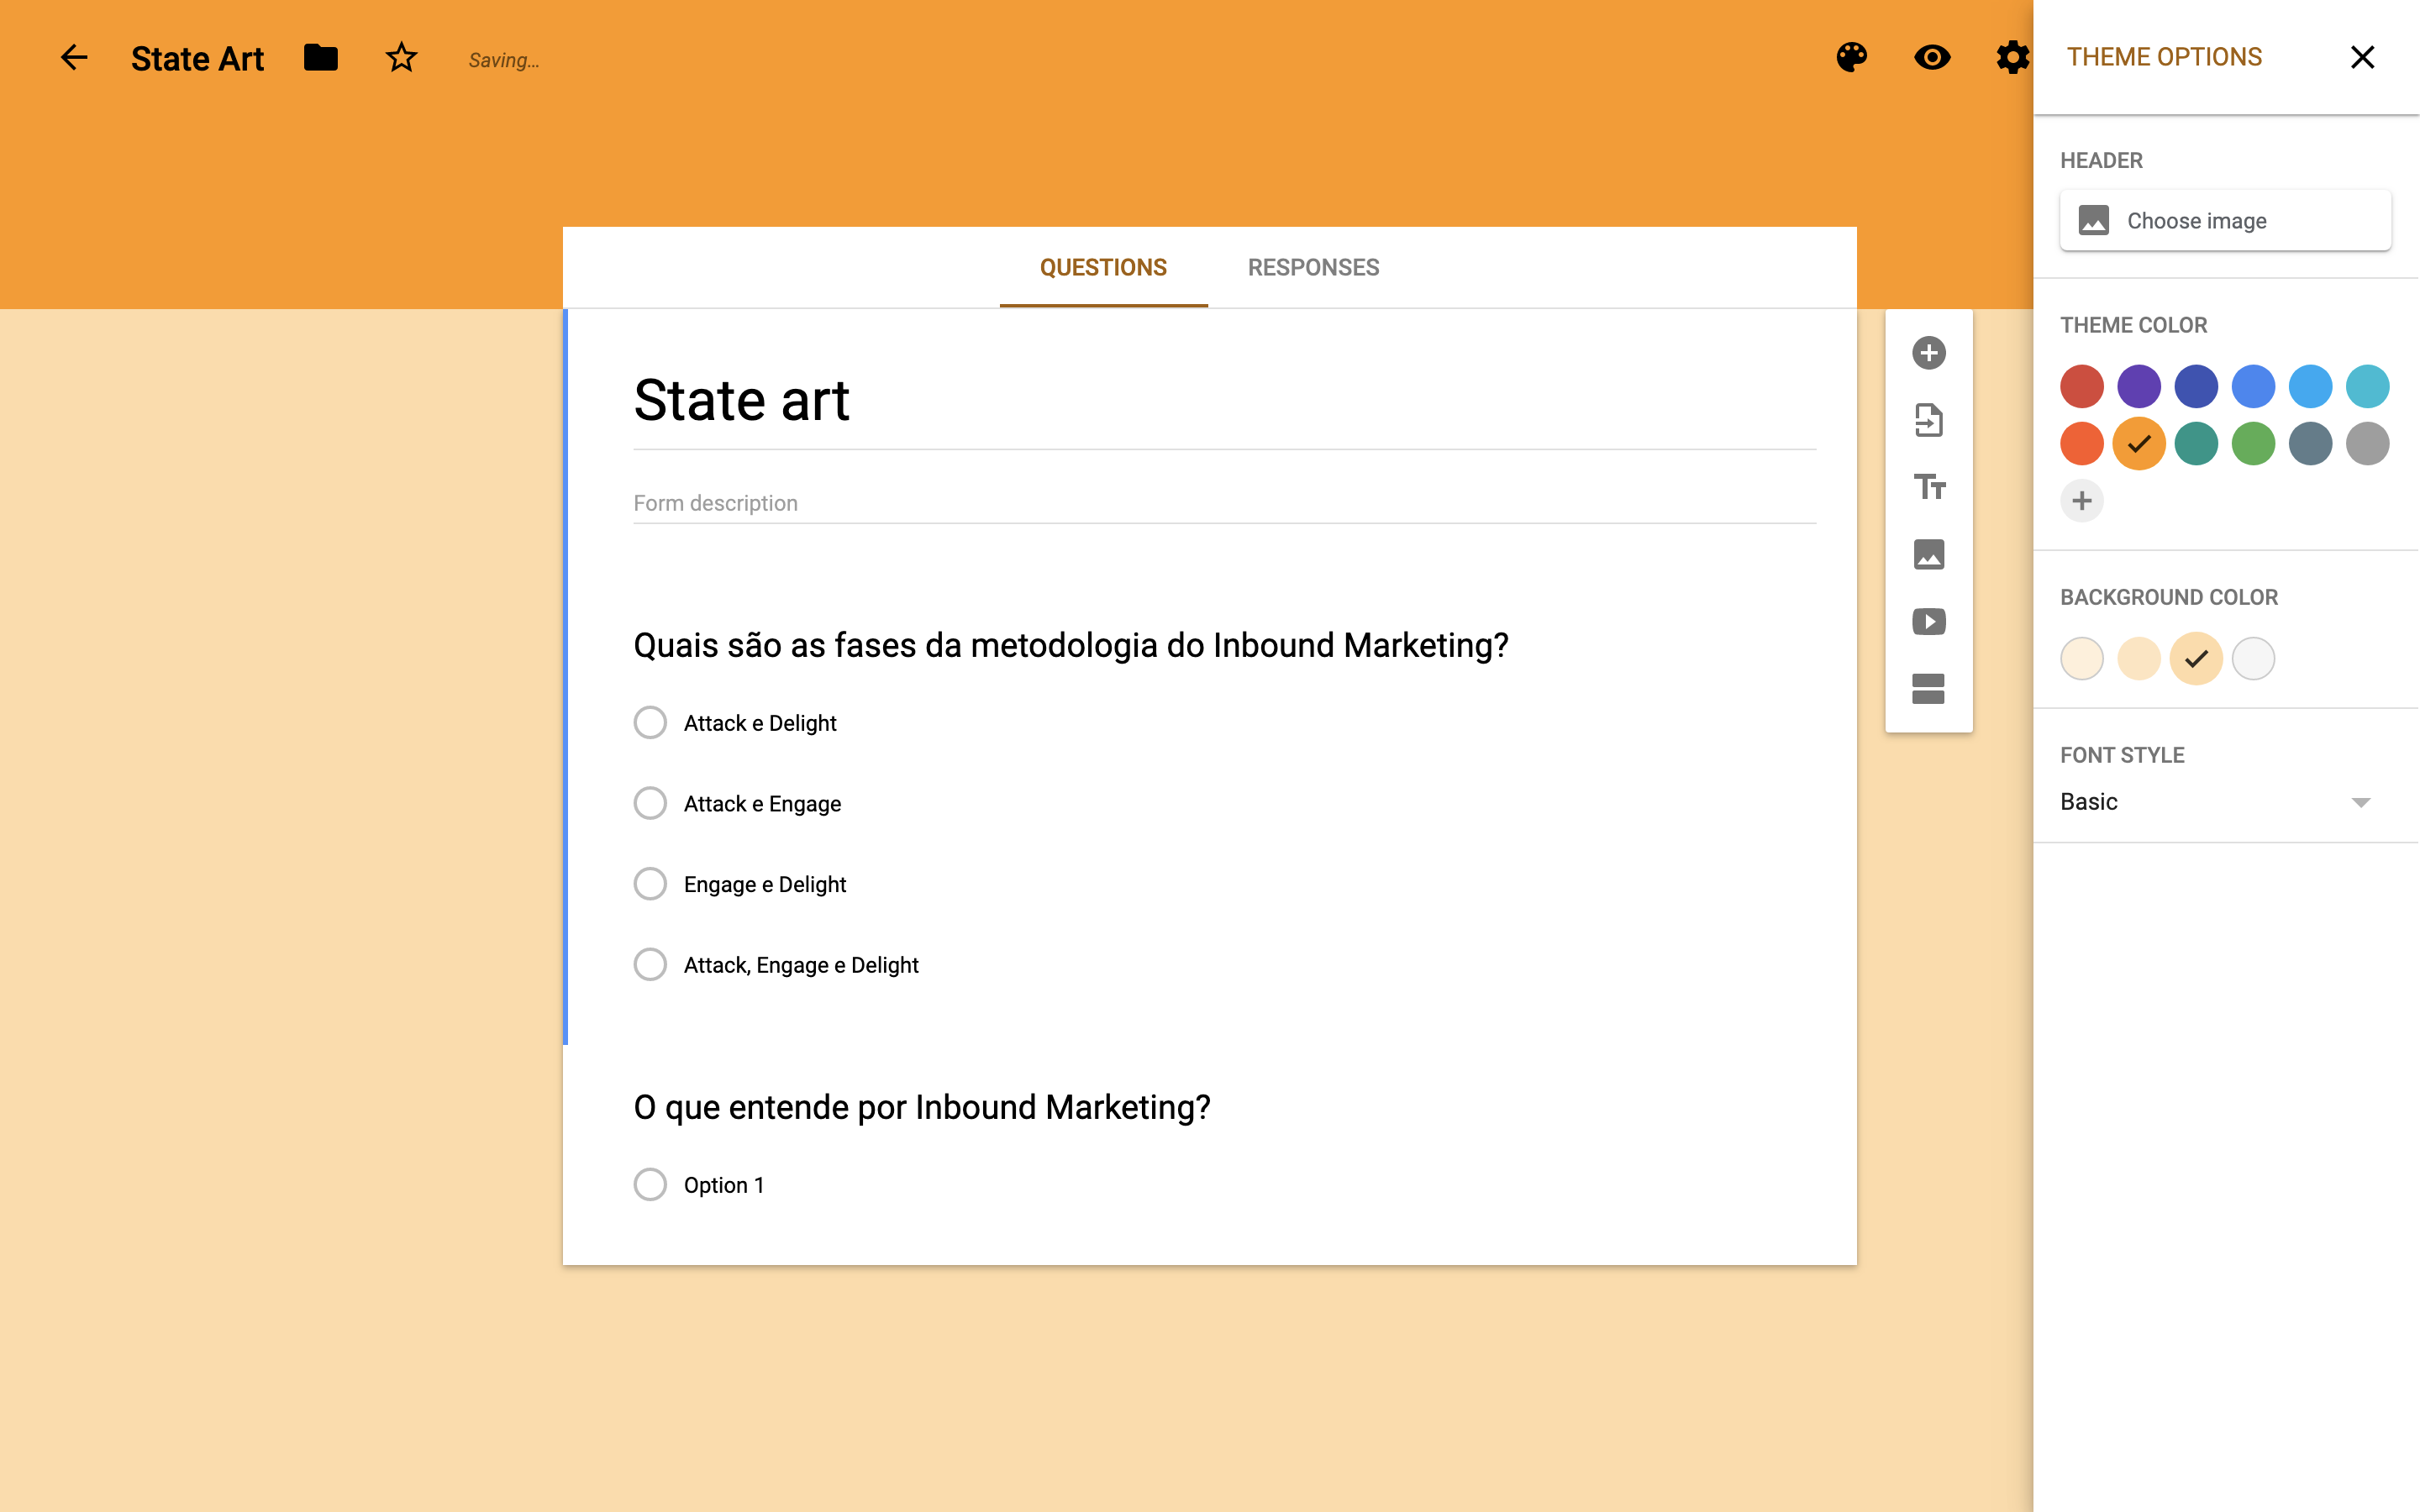
\includegraphics[width=1\textwidth]{img/gf/gf-form-design}
		\caption{Google Form - Alterar design do formulário}
		\label{fig:gf-form-design}
	\end{center}
\end{figure}

\newpage

Grande parte das plataformas e aplicações,no mercado, de criação de formulários permitem personalizar os formulários, ao gosto do utilizador, e o Google Form não é excepção. A aplicação permite alterar as definições padrão do formulário(Figuras \ref{fig:gf-form-set1}, \ref{fig:gf-form-set2} e \ref{fig:gf-form-set3}) e, apesar de se poder também personalidar o \textit{design} do formulário (\ref{fig:gf-form-design}), apens podemos alterar a cor ou imagem de fundo e fonte de texto.

\begin{figure}[ht!]
	\begin{center}
		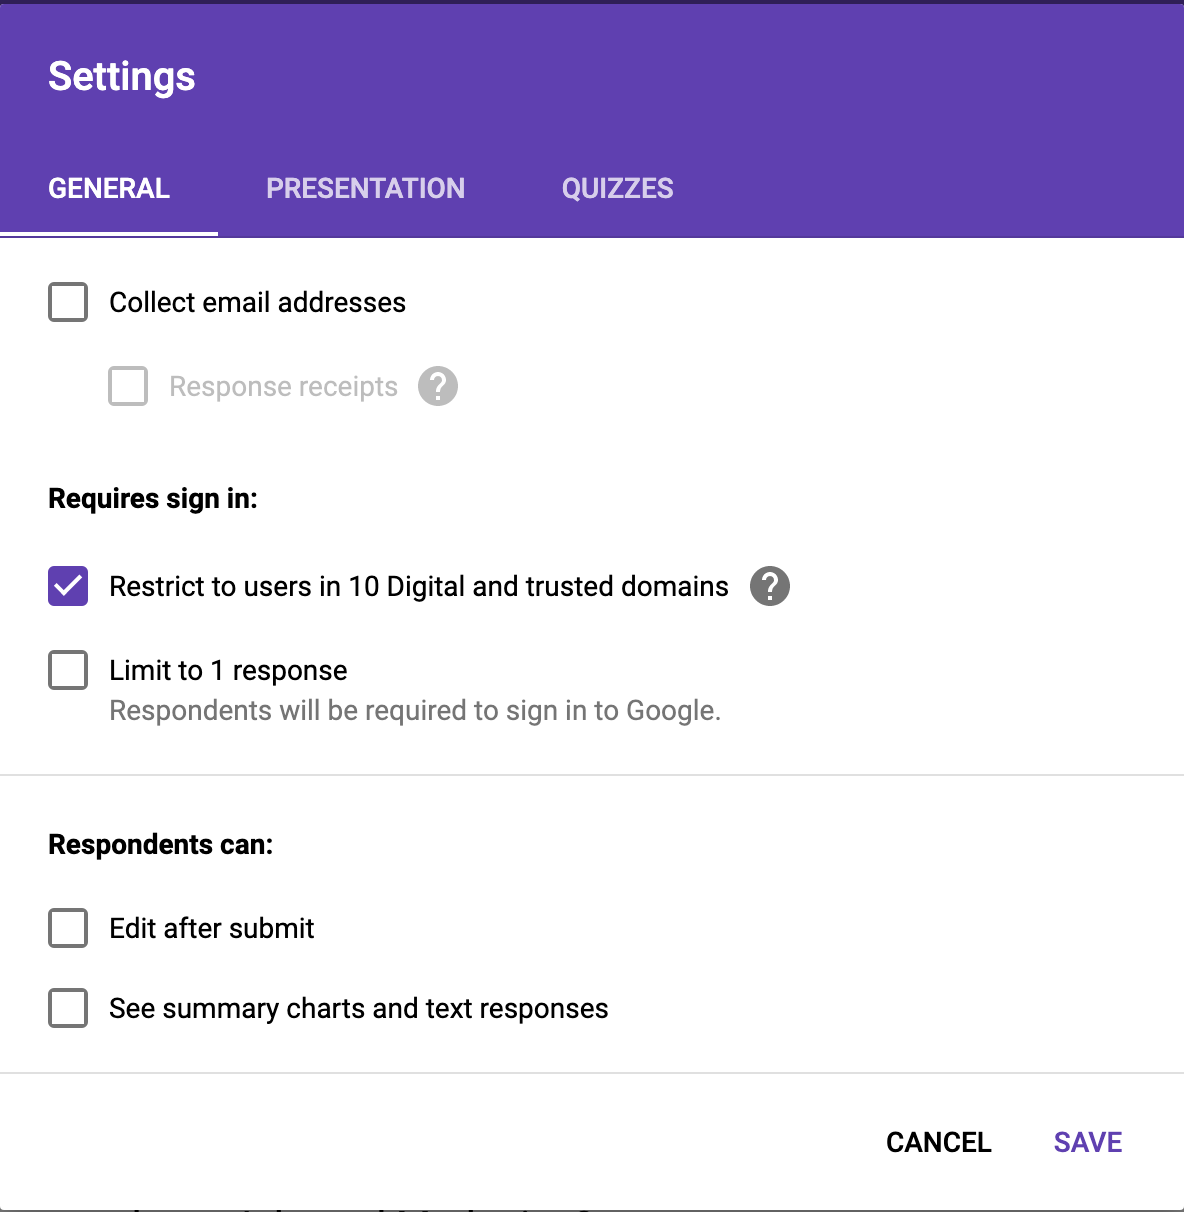
\includegraphics[height=.30\textheight]{img/gf/gf-form-set1}
		\caption{Google Form - Opções}
		\label{fig:gf-form-set1}
	\end{center}
\end{figure}

\begin{figure}[ht!]
	\begin{center}
		\begin{minipage}{0.40\textwidth}
			\begin{center}
				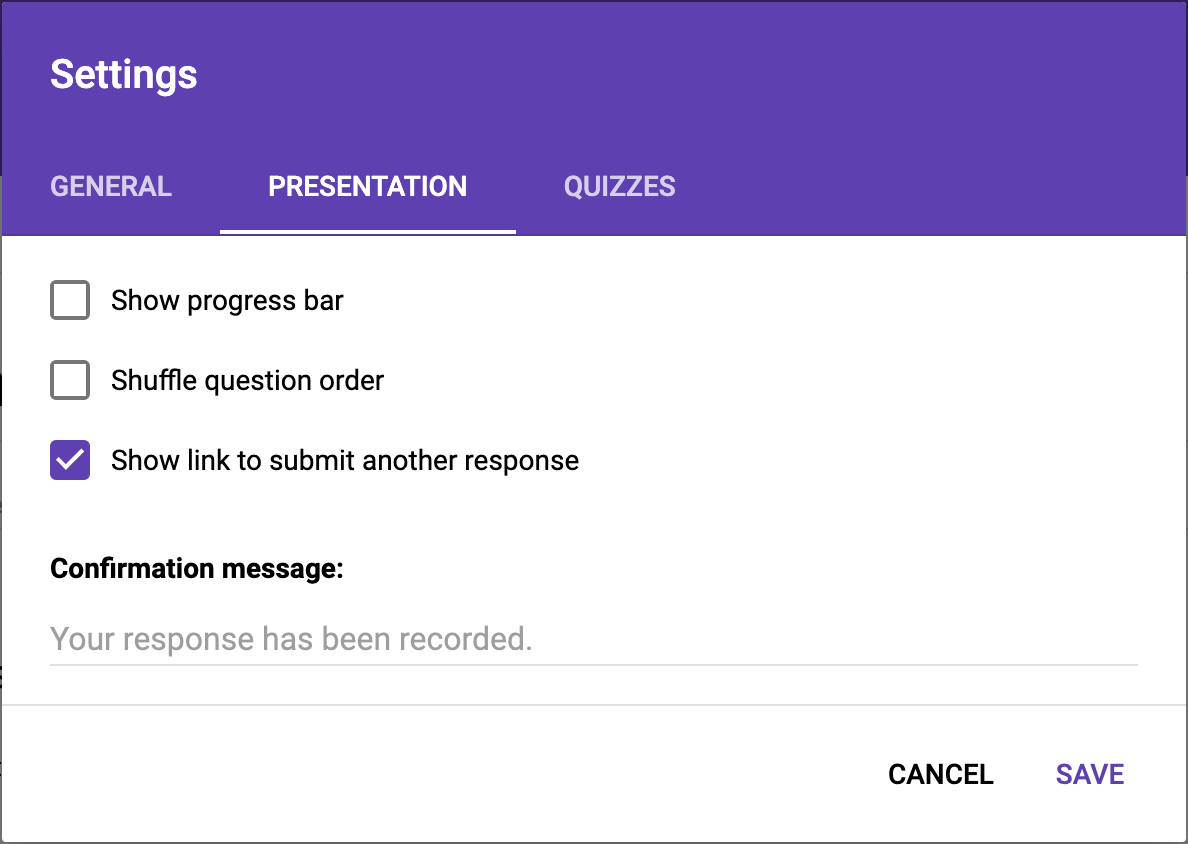
\includegraphics[height=.22\textheight]{img/gf/gf-form-set2}
				\caption{Google Form - Opções}
				\label{fig:gf-form-set2}
			\end{center}
		\end{minipage}
		\hspace{2cm}
		\begin{minipage}{0.40\textwidth}
			\begin{center}
				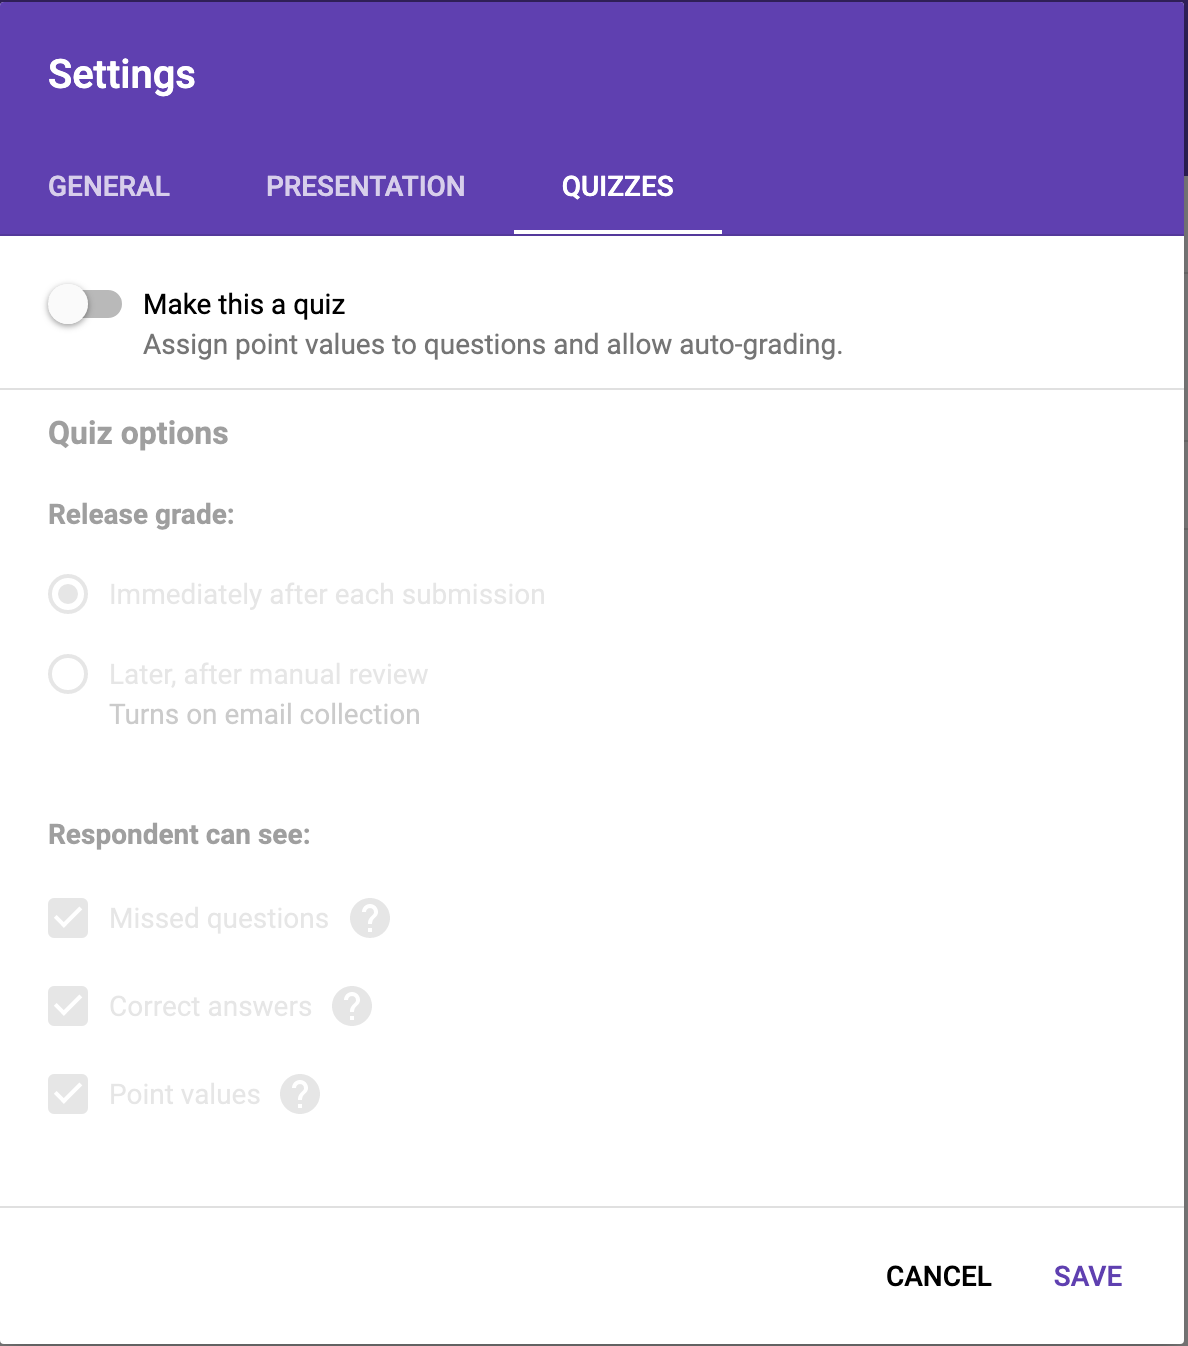
\includegraphics[height=.30\textheight]{img/gf/gf-form-set3}
				\caption{Google Form - Opções}
				\label{fig:gf-form-set3}
			\end{center}
		\end{minipage}
	\end{center}
\end{figure}

Antes de partilhar o formulário, precisamos de verificar se o formulário ficou construido como planeado e para isso a aplicação fornece a funcionalidade: \textit{preview}. O Google Form permite os utilizadores enviarem o formulário através de um link, por email, embebido num pagina web ou partilhando no Facebook ou Tweeter utilizando os botões de partilha rápida.

Na análise de resultados, como podemos ver na Figura \ref{fig:gf-form-results} a aplicação faz uma exibição do resumo das respotas, mostrando alguns gráficos/estatisticas contudo, o utilizador não dispõe de nenhuma funcionalidade que filtra ou segmenta os dados. A unica maneira que o utilizador tem de poder tratar os dados e segmenta-los é, depois de exportar os dados, utilizando o Google Sheets, que já requer algum conhecimento na ferramenta. 


\begin{figure}[ht!]
	\begin{center}
		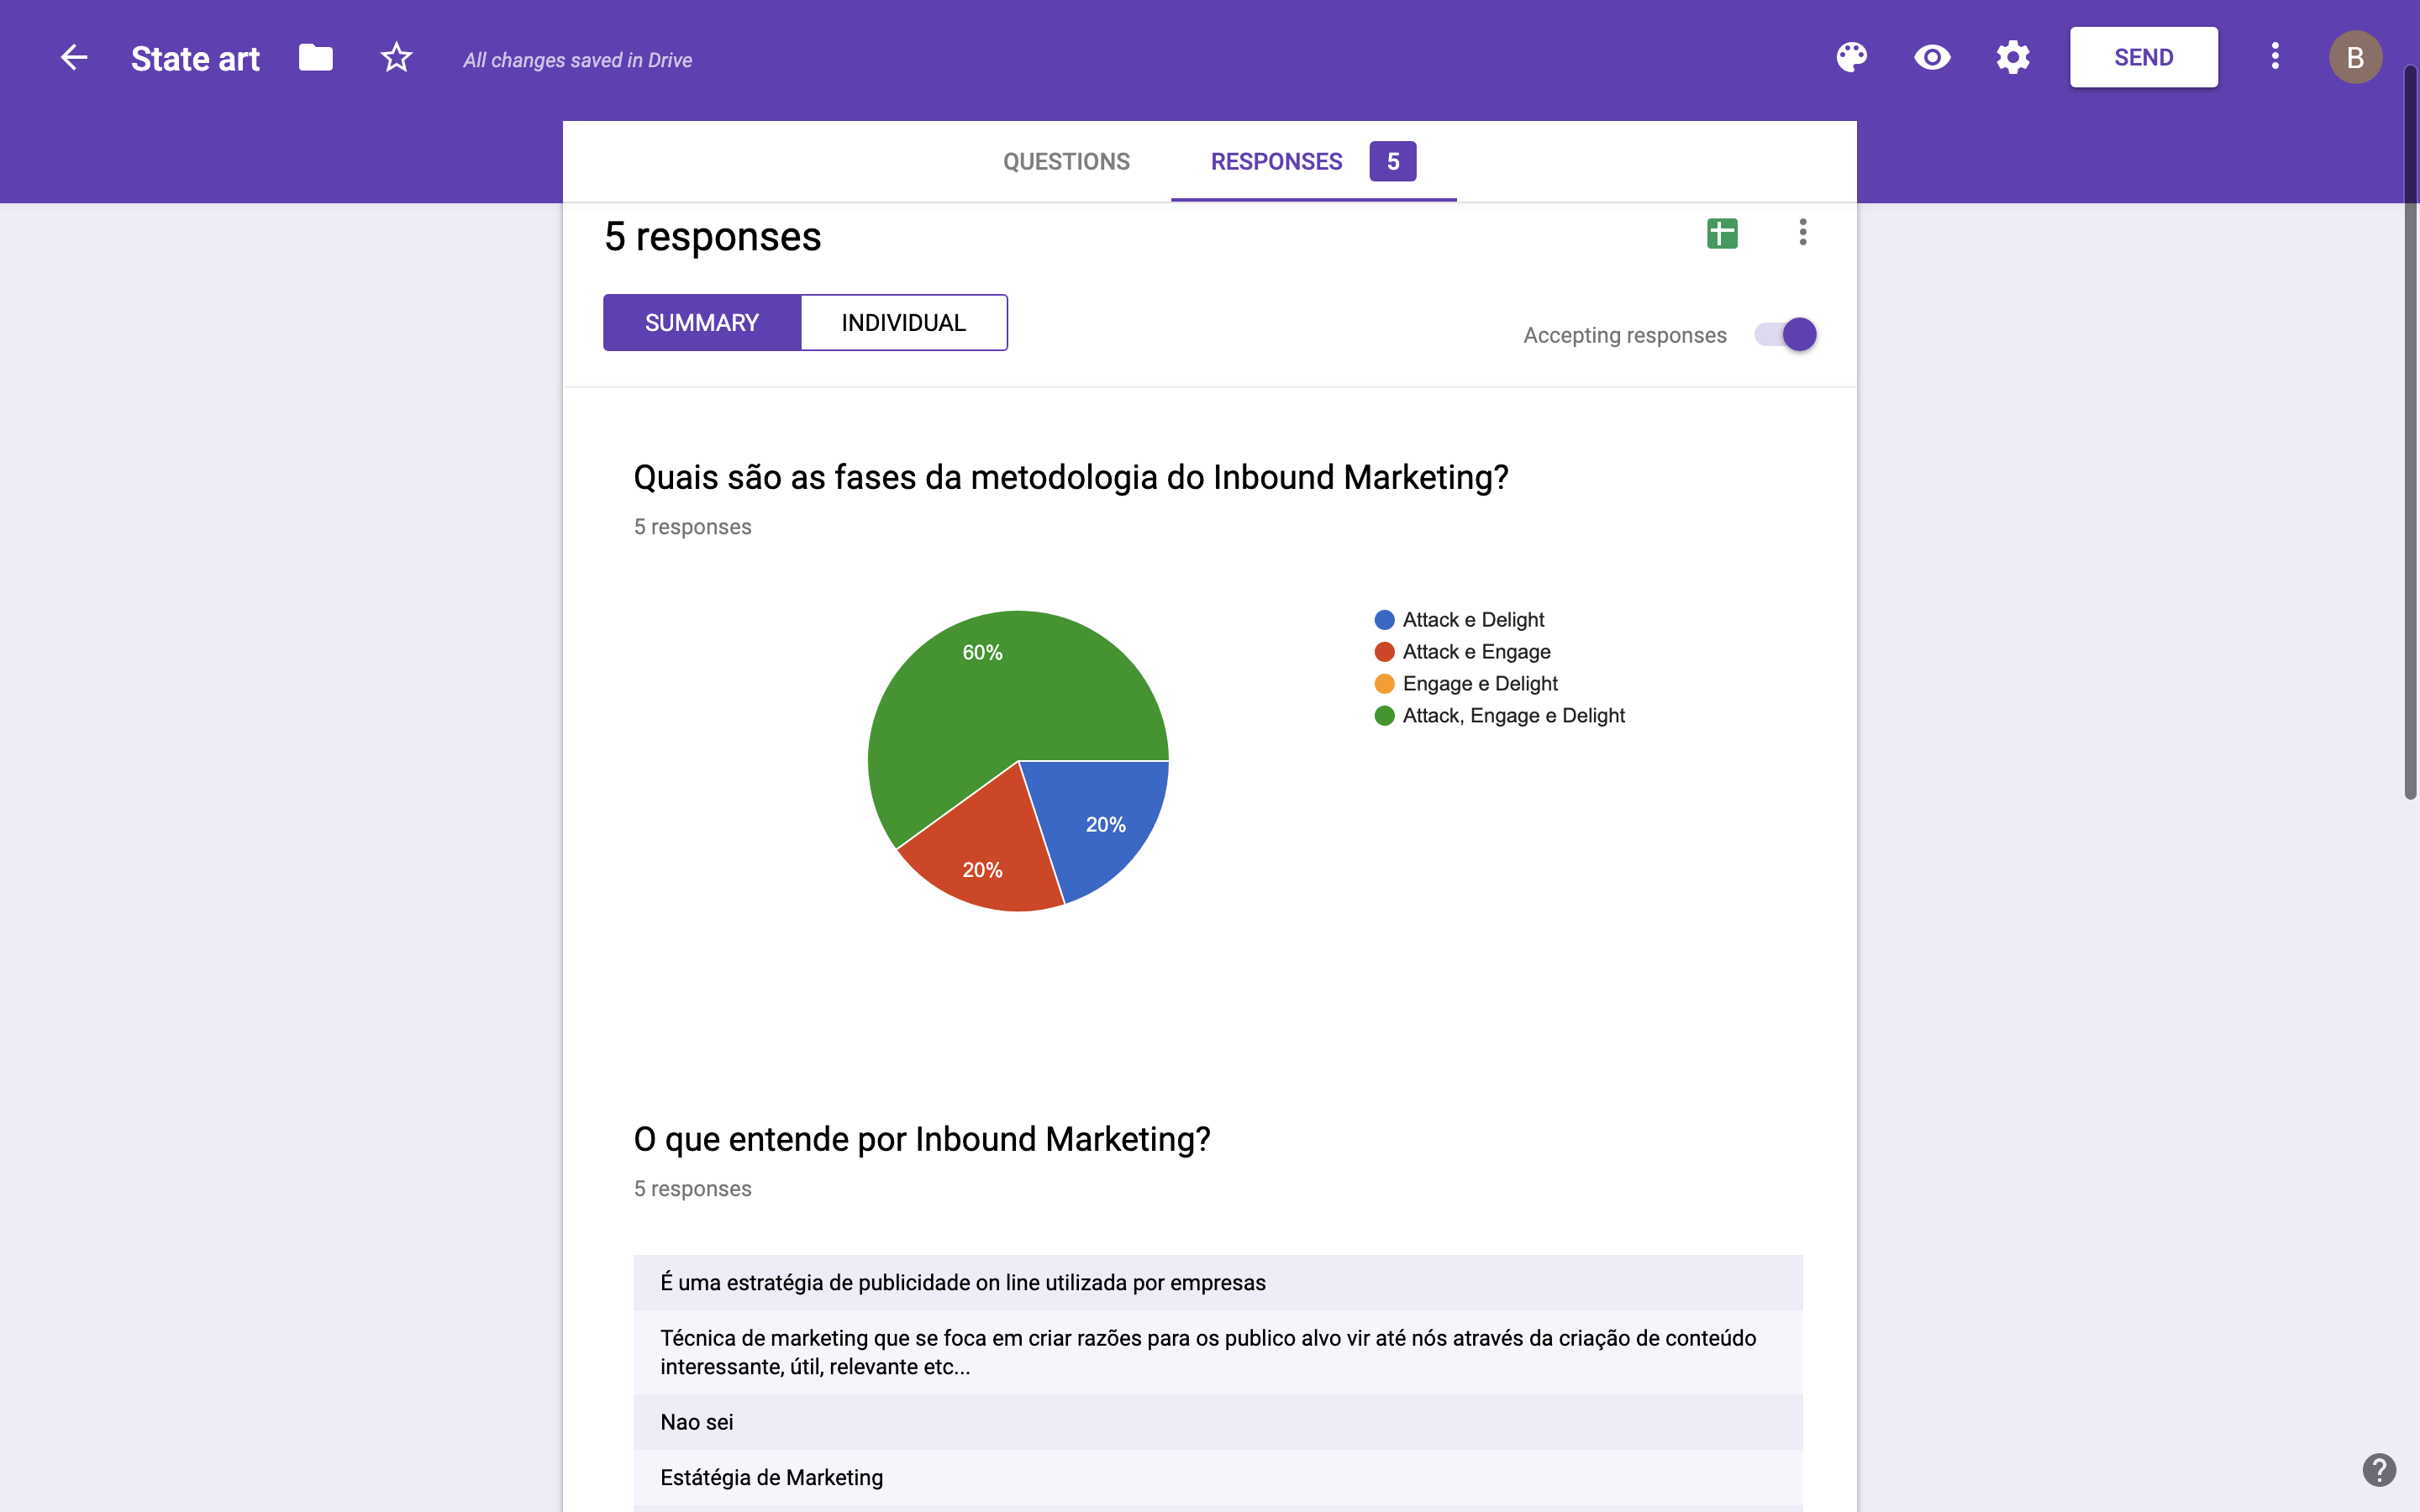
\includegraphics[width=1\textwidth]{img/gf/gf-form-results}
		\caption{Google Form - Sumério dos resultados obtidos}
		\label{fig:gf-form-results}
	\end{center}
\end{figure}


\section{Comparação de Aplicações}
\label{comparacao}

Na Tabela \ref{tab:comparacao} encontra-se a comparação entre as ferramentas analisadas nos secções \ref{surveyMonkey}, \ref{typeform} e \ref{googleform}, baseada numa lista de funcionalidades.

Como vimos anteriormente em todas as plataformas/ferramentas é necessário criar uma conta para aceder a todas as funcionalides e em todas as plataformas analisadas é possível criar conta e iniciar sessão através de sistemas externos (\acrshort{api}). O Projecto a desenvolver segue um modelo \acrshort{b2b} e por isso mesmo não é de grande importancia implementar esse tipo de funcionalidades pelo que, devido à sua relevância, não foi referido na Tabela \ref{tab:comparacao}.

O plataforma da Google fornece, no plano gratuito, todas as funcionalidades, ao contrário de todas as ferramentas analisadas anteriormente, que, tal como se passará com a plataforma a desenvolver, para se ter acesso a todas as funcionalidades, ou pacotes de funcionalidades, terá de ser paga uma subscrição.

Todas as platafomas permitem a criação de formulários do zero, e a plataforma da 10.digital não é excepção. Tal como foi definido na estratégia de negócio, os conteúdos que serão lançados nos formulários não serão da autoridade da 10.digital, a mesmos que estejamos incluídos em algum projecto relazionado. Dito isto facilmente se decidiu que a plataforma a desenvolver terá, tal como todas as outras ferramentas analisadas, a funcionalidade de poder adicionar conteúdo previamente feito de forma rápido (i. e. adicionar um ficheiro com todo o conteúdo estruturado). 


Tal como foi referido no capítulo \ref{sec:introducao}, secção \ref{subsec:contexto}, o inbound é uma estratégia de marketing que se foca em criar razões para os publico alvo vir até nós através da criação de conteúdo interessante, útil, relevante etc... Para manter esta procura por parte dos clientes é necessário haver valor ao longo da jornada e ideialmente proporcionar uma boa experiência ao utilizador. Nesta medida a personalização dos formulários é muito importante tanto a nível de conteúdo como estético e funcional para que o utilizador se sinta valorizado. Para tornar isto possível, tal como o SurveyMonkey e o Typoform, a plataforma a desenvolver será a algumas funcionalidades que lhe permitirá criar vários tipos de pergunta e estéticamente melhorar a experiência do utilizador final.


Antes de enviar/partilhar um formulário é 

\newpage

		\renewcommand{\arraystretch}{2.5}
		\setlength\arrayrulewidth{1.5pt}
	\begin{table}[!ht]  
		\centering
		\begin{tabular}{|p{4cm}|p{1.5cm}|p{1.5cm}|p{1.5cm}|p{1.5cm}|}
			\cline{2-5}
			\multicolumn{1}{c|}{} & \hspace{0.6cm}\begin{sideways}SurveyMonkey.\end{sideways} & \hspace{0.6cm}\begin{sideways}Typeform\end{sideways} & \hspace{0.6cm}\begin{sideways}Google Form\end{sideways} &\hspace{0.6cm}\begin{sideways} 10.digital\end{sideways}\\ \hline
			
			Plano Gratuito & \cellcolor{yellow!80}   & \cellcolor{yellow!80}  & \cellcolor{green!80} & \cellcolor{yellow!80}  \\ \hline
			
			Criar Formulário do zero & \cellcolor{green!80}  & \cellcolor{green!80}  & \cellcolor{green!80} & \cellcolor{green!80} \\ \hline
			
			Templates de formulários disponíveis& \cellcolor{green!80}  & \cellcolor{green!80} & \cellcolor{green!80} & ???? \\ \hline
			
			Adicionar conteúdo previamente feitos & \cellcolor{green!80}   & \cellcolor{red!80}  & \cellcolor{green!80} & \cellcolor{green!80}  \\ \hline
			
				Tipos de perguntas & \cellcolor{green!80}  & \cellcolor{green!80}  & \cellcolor{yellow!80} & \cellcolor{green!80}  \\ \hline
			
			% Recomendações de perguntas& \cellcolor{green!80}  & \cellcolor{green!80}  & \cellcolor{blue!25} & \cellcolor{blue!25}  \\ \hline
			
			\textit{Drag and Drop} & \cellcolor{green!80}   & \cellcolor{red!80}  & \cellcolor{red!80} & \cellcolor{red!80} \\ \hline
			
			Personalização do formulário& \cellcolor{green!80}    & \cellcolor{green!80}   & \cellcolor{yellow!80} & \cellcolor{green!80}   \\ \hline
			
			 Pré-visualização do formulário& \cellcolor{green!80}  & \cellcolor{green!80}  & \cellcolor{green!80} & \cellcolor{green!80} \\ \hline
			
			 Integração de sistemas externos& \cellcolor{red!80}   & \cellcolor{green!80} & \cellcolor{yellow!80}  & ????  \\ \hline
			
			Envio do formulário de forma periódica & \cellcolor{red!80}   & \cellcolor{red!80}  & \cellcolor{red!80} & \cellcolor{green!80} \\ \hline
			
			 Analise de resultados & \cellcolor{green!80}   & \cellcolor{yellow!80} & \cellcolor{yellow!80} & \cellcolor{green!80}  \\ \hline
			
			Partilha dos resultados & \cellcolor{green!80}   & \cellcolor{green!80}   & \cellcolor{green!80}  & ???? \\ \hline
			
			Exportar os resultados & \cellcolor{green!80}   & \cellcolor{green!80}   & \cellcolor{green!80}  & \cellcolor{green!80}  \\ \hline
			
			
		\end{tabular}
	\caption{Tabela de comparações de funcionalidades}
	\label{tab:comparacao}

	\end{table}


%-------------------------------------------------------------------------------------------------
\blankpage
%-------------------------------------------------------------------------------------------------

\glsresetall



